\documentclass[10pt]{article} % For LaTeX2e
\usepackage[preprint]{tmlr}
% If accepted, instead use the following line for the camera-ready submission:
%\usepackage[accepted]{tmlr}
% To de-anonymize and remove mentions to TMLR (for example for posting to preprint servers), instead use the following:
%\usepackage[preprint]{tmlr}

\usepackage{amsmath,amssymb,amsthm}
\usepackage{graphicx}
\graphicspath{{../figures/}}
\usepackage{booktabs}
\usepackage{multirow}
\usepackage{enumitem}  % For tighter list spacing
\setlist{nosep}  % Remove extra spacing in lists
\usepackage{url}
\usepackage{algorithm}
\usepackage{algpseudocode}
\usepackage{xcolor}
\usepackage{tcolorbox}
\tcbuselibrary{breakable}  % Allow boxes to break across pages
\usepackage{float}
\usepackage{placeins}  % For \FloatBarrier when needed
\usepackage{listings}

% Float parameters to reduce whitespace
\renewcommand{\topfraction}{0.9}      % Max fraction of page for floats at top
\renewcommand{\bottomfraction}{0.9}   % Max fraction of page for floats at bottom
\renewcommand{\textfraction}{0.1}     % Min fraction of page for text
\renewcommand{\floatpagefraction}{0.8} % Min fraction of float page that must be floats
\setcounter{topnumber}{3}             % Max floats at top of page
\setcounter{bottomnumber}{3}          % Max floats at bottom of page
\setcounter{totalnumber}{6}           % Max floats per page

% Code listing style for appendix
\definecolor{codegreen}{rgb}{0,0.6,0}
\definecolor{codegray}{rgb}{0.5,0.5,0.5}
\definecolor{codepurple}{rgb}{0.58,0,0.82}
\definecolor{backcolour}{rgb}{0.98,0.98,0.98}

\lstdefinestyle{pythonstyle}{
    backgroundcolor=\color{backcolour},
    commentstyle=\color{codegreen},
    keywordstyle=\color{blue},
    numberstyle=\tiny\color{codegray},
    stringstyle=\color{codepurple},
    basicstyle=\ttfamily\footnotesize,
    breakatwhitespace=false,
    breaklines=true,
    captionpos=b,
    keepspaces=true,
    numbers=left,
    numbersep=5pt,
    showspaces=false,
    showstringspaces=false,
    showtabs=false,
    tabsize=2,
    language=Python
}
\lstset{style=pythonstyle}

% Theorem environments (amsthm)
\theoremstyle{plain}
\newtheorem{theorem}{Theorem}[section]
\newtheorem{proposition}[theorem]{Proposition}
\newtheorem{lemma}[theorem]{Lemma}
\newtheorem{corollary}[theorem]{Corollary}

\theoremstyle{definition}
\newtheorem{definition}[theorem]{Definition}
\newtheorem{example}[theorem]{Example}
\newtheorem{remark}[theorem]{Remark}

% Commands
\newcommand{\CF}{\mathrm{CF}}
\newcommand{\IC}{\mathrm{IC}}  % Inference Coupling
\newcommand{\BB}{\mathcal{B}}  % Balance Factor
\newcommand{\CC}{\mathrm{CC}}  % Control Coupling
\newcommand{\MI}{I}
\newcommand{\Ent}{H}
\newcommand{\KL}{D_{\mathrm{KL}}}
\newcommand{\E}{\mathbb{E}}
\newcommand{\Var}{\mathrm{Var}}
\newcommand{\MF}{\mathrm{MF}}
\newcommand{\Cov}{\mathrm{Cov}}
\newcommand{\R}{\mathbb{R}}

\title{Circulatory Fidelity: A Relational Theory of Information Flow in Hierarchical Models}

% Authors must not appear in the submitted version. They should be hidden
% as long as the tmlr package is used without the [accepted] or [preprint] options.
% Non-anonymous submissions will be rejected without review.

\author{\name Aaron Lowry \\
      \addr Independent Researcher}

% The \author macro works with any number of authors. Use \AND 
% to separate the names and addresses of multiple authors.

\date{January 4, 2026}

\begin{document}

\maketitle

\begin{center}
{\large Version 1.1 --- January 4, 2026}
\end{center}
\vspace{-1em}

\begin{abstract}
While Mean-Field Variational Inference (MFVI) enables scalable Bayesian computation, its independence assumption systematically severs the relational coupling required for accurate posterior estimation, often leading to silent failure. This paper introduces \emph{Circulatory Fidelity}, a pre-inference diagnostic framework grounded in the precision matrix decomposition $\Lambda = D + R$, which quantifies the information-theoretic cost of discarding relational structure ($R$) before computational resources are committed.

In this decomposition, $D$ (diagonal) captures \emph{nodal} structure and $R$ (off-diagonal) captures \emph{relational} structure. MFVI keeps $D$ but discards $R$. The \textbf{Relational Invariance Theorem} proves that for Gaussian systems, mutual information $I(Z;X) = -\frac{1}{2}\log(1-\rho^2)$ depends \emph{only} on correlation $\rho$---not on marginal variances $\sigma_z^2$ or $\sigma_x^2$. This yields \textbf{Inference Coupling} $\IC = |\rho|$ as the primary pre-inference diagnostic. The companion \textbf{Balance Factor} $\BB$ characterizes architectural symmetry but adds no predictive value for MFVI failure ($\Delta R^2 \approx 0$). \textbf{Control Coupling} $\CC = |\rho| \cdot (\sigma_i/\sigma_j)$ captures directional intervention leverage, where scale \emph{does} matter---this is where the ``bottleneck'' principle applies.

We establish four additional contributions: (1) The \textbf{Computational Synergy Principle}---for discrete Boolean functions, synergistic dependencies arise when the generative function is affine over $\text{GF}(2)$, enabling a two-stage diagnostic where pairwise $\IC \approx 0$ combined with interaction $\IC > 0$ identifies XOR-type structure (with the formal equivalence holding exactly in the Boolean uniform-input case). (2) The \textbf{Dependency Asymmetry}---high IC predicts MFVI failure in filtering models but hierarchy redundancy in pooling models, resolved by distinguishing constitutive from inductive coupling. (3) The \textbf{Proximal Dominance Principle}---in deep hierarchies with fully factorized mean-field approximations, proximal coupling causes up to $40\times$ degradation when severed while distal coupling causes exactly $1.0\times$ when severed if the proximal layer is also severed (mathematically guaranteed); however, distal coupling amplifies proximal failure by $1.01$--$2.26\times$ when both are present ($N = 16{,}000$). (4) The \textbf{Maximal Coupling Rule}---for non-stationary series, MFVI suitability depends on $\IC_{\max}$, not global average.

Validation spans stochastic volatility filters ($r = 0.86$ for log-likelihood gap, $N = 8{,}000$), hierarchical linear models, and three-layer hierarchies ($N = 32{,}000$+ total), yielding a practical pre-inference workflow. The relational theory clarifies a fundamental asymmetry: \emph{what you can learn} from a relationship (inference) depends only on coupling strength, while \emph{what you can do} through a relationship (control) depends on both coupling and scale.
\end{abstract}

%=============================================================================
\section{Introduction: The Pre-Inference Diagnostic Gap}
\label{sec:intro}
%=============================================================================

Variational inference (VI) has become essential for approximate Bayesian computation, offering scalable alternatives to Markov Chain Monte Carlo \citep{blei2017variational}. The mean-field assumption---that the variational distribution factorizes as $q(\theta) = \prod_i q_i(\theta_i)$---enables tractable optimization but enforces statistical independence between all latent variables.

This paper addresses a practical question: \emph{before committing computational resources to posterior inference}, can we assess whether MFVI is appropriate for a given model?

The ELBO (Evidence Lower Bound) is the optimization objective \emph{during} variational inference---it is the loss function being maximized throughout training \citep{blei2017variational}. While ELBO values can be compared post-inference, they cannot predict \emph{before} inference whether MFVI will succeed. Other diagnostics also operate \emph{after} inference completes:
\begin{itemize}
    \item \textbf{PSIS-$\hat{k}$}: Diagnoses importance sampling reliability but requires posterior samples \citep{vehtari2017practical}
    \item \textbf{SBC}: Simulation-based calibration checks posterior calibration but requires fitting hundreds of simulated datasets \citep{talts2018validating}
\end{itemize}

\subsection{The Relational Insight}

We introduce \textbf{Circulatory Fidelity} (CF), a framework for pre-inference diagnostics grounded in a fundamental distinction: MFVI failure depends entirely on \emph{relational structure}---the coupling between variables---not on \emph{nodal structure}---individual variable properties like marginal variances.

\begin{tcolorbox}[colback=blue!5, colframe=blue!50!black, title=\textbf{Notation: CF Framework vs.\ IC Diagnostic}]
\textbf{Circulatory Fidelity (CF)} refers to the overall diagnostic \emph{framework}---the theoretical apparatus including the relational theory, companion metrics, and practical workflow.

\textbf{Inference Coupling (IC)} is the primary \emph{diagnostic metric} within this framework. For Gaussians: $\IC = |\rho|$.

\textbf{Historical note:} The original v1.0 formulation defined $\text{CF} = I(Z;X)/\min(H(Z), H(X))$. The Relational Invariance Theorem (Theorem~\ref{thm:relational-invariance}) proves this normalization is unnecessary for Gaussian inference diagnostics---the marginal entropies cancel. The current formulation uses IC = $|\rho|$ as the primary diagnostic, equivalent to the Linfoot correlation.
\end{tcolorbox}

For a multivariate Gaussian with covariance $\Sigma$, the precision matrix $\Lambda = \Sigma^{-1}$ decomposes as:
\begin{equation}
\Lambda = D + R
\label{eq:decomposition}
\end{equation}
where $D = \text{diag}(\Lambda)$ captures nodal structure and $R = \Lambda - D$ captures relational structure. Mean-field variational inference \emph{keeps} $D$ but \emph{discards} $R$---a phenomenon rigorously characterized by \citet{giordano2018covariances}, who proved that MFVI systematically underestimates posterior covariances. IC provides a pre-inference metric that predicts when this covariance underestimation will be fatal: high IC indicates that the discarded relational structure $R$ contains information essential for accurate posterior approximation. The fundamental question becomes: how much does discarding $R$ cost?

We prove (Theorem~\ref{thm:relational-invariance}) that for Gaussian systems, the mutual information---and hence the KL cost of mean-field factorization---is:
\begin{equation}
I(Z; X) = -\frac{1}{2}\log(1 - \rho^2)
\end{equation}
The marginal variances $\sigma_z^2$ and $\sigma_x^2$ \emph{cancel completely}. This yields \textbf{Inference Coupling} as the primary diagnostic:
\begin{equation}
\IC(z, x) = \frac{|\Lambda_{zx}|}{\sqrt{\Lambda_{zz} \cdot \Lambda_{xx}}} = |\rho|
\label{eq:ic}
\end{equation}
For Gaussian systems, IC equals the absolute Pearson correlation. IC measures exactly what MFVI discards: the normalized relational structure.

\paragraph{The ``Circulatory'' metaphor.} While generative models define unidirectional information flow ($z \to x$), \emph{inference} requires bidirectional message passing: the likelihood signal propagates upward ($x \to z$), and the prior signal propagates downward ($z \to x$). This bidirectional flow is formalized in belief propagation as the exchange of messages between factor graph nodes; mean-field factorization blocks these messages at every edge, severing the circuit. ``Circulatory Fidelity'' measures the capacity of the model's structure to support this necessary message passing; high IC indicates that factorization will severely impair the inference circuit.

\paragraph{Key insight.} IC is computable \emph{before} observing data, directly from model structure. By simulating from the prior predictive $p(\theta, z, x) = p(\theta)p(z|\theta)p(x|z)$, we obtain samples where IC can be estimated via copula correlation. This diagnoses whether the \emph{model itself} creates dependencies that MFVI cannot represent.

\paragraph{Inference vs.\ Control.} The relational theory clarifies a fundamental asymmetry:
\begin{itemize}
    \item \textbf{Inference} (what you can learn): depends only on $\IC = |\rho|$
    \item \textbf{Control} (what you can do): depends on $\CC = |\rho| \times (\sigma_i / \sigma_j)$
\end{itemize}
The ``bottleneck'' principle---that the lower-capacity variable limits information transfer---applies to \emph{control}, not inference. For MFVI diagnostics, only IC matters.

\paragraph{Contributions.} We present five theoretical contributions:
\begin{enumerate}
    \item \textbf{The Relational Theory:} We prove that inference quality depends only on relational structure (IC), not nodal structure (marginal variances). The Relational Invariance Theorem establishes that $I(Z;X) = -\frac{1}{2}\log(1-\rho^2)$ depends only on $\rho$. The Balance Factor $\BB$ characterizes architecture but adds $\Delta R^2 \approx 0$ for predicting MFVI failure. Control Coupling $\CC$ captures directional intervention leverage where scale \emph{does} matter. (Section~\ref{sec:definition})
    \item \textbf{The Computational Synergy Principle and Two-Stage Protocol:} Synergy-generating functions are characterized algebraically as affine over $\text{GF}(2)$, connecting to Siegenthaler's correlation immunity. This equivalence enables a two-stage diagnostic: pairwise IC detects standard coupling, while $\IC_{\text{pairwise}} \approx 0$ combined with $\IC_{\text{interaction}} > 0$ positively identifies XOR-type structure (Theorem~\ref{thm:synergy}, Section~\ref{sec:synergy})
    \item \textbf{The Dependency Asymmetry and Structural Taxonomy:} High IC predicts MFVI failure in filtering models (constitutive coupling) but hierarchy redundancy in pooling models (inductive coupling), resolved through a taxonomy distinguishing load-bearing from scaffolding dependencies (Section~\ref{sec:taxonomy})
    \item \textbf{The Proximal Dominance Principle:} In deep hierarchies, proximal coupling drives up to $40\times$ degradation (95\% CI: 2.7--102) while distal coupling causes exactly $1.0\times$ (mathematically guaranteed). This implies that for $L$-layer models, only the proximal layer requires IC analysis, reducing diagnostic complexity from $O(L^2)$ to $O(1)$. For non-stationary time series, we derive the corollary \emph{Maximal Coupling Rule}: MFVI suitability is determined by $\IC_{\max}$, not global average (Sections~\ref{sec:deep},~\ref{sec:windowed})
    \item \textbf{The Linfoot Equivalence:} For Gaussian systems, $\IC = r_L$ where $r_L = \sqrt{1 - \exp(-2I)}$ is the Linfoot informational correlation, providing a coordinate-invariant formulation that extends to non-Gaussian distributions (Section~\ref{sec:linfoot})
\end{enumerate}
These contributions are supported by empirical validation ($N = 32{,}000$+ simulations) and synthesized into a practical prior predictive workflow (Section~\ref{sec:workflow}).

\paragraph{Scope and Limitations.} IC operates on pairs of variables or variable groups. Mean-field variational inference can fail due to either (a) strong pairwise dependencies or (b) synergistic higher-order dependencies where information emerges only from joint configurations. The \emph{two-stage diagnostic protocol} addresses both failure modes: Stage 1 (pairwise IC) detects standard coupling; Stage 2 (interaction IC) detects synergistic structure. Critically, the signature of pairwise $\IC \approx 0$ combined with interaction $\IC > 0$ \emph{positively identifies} XOR-type algebraic structure through the Computational Synergy Principle (Theorem~\ref{thm:synergy}). This transforms synergy from a ``blind spot'' into a precisely detectable pattern. We formalize this protocol in Section~\ref{sec:synergy}.

\paragraph{Paper organization.} We structure the exposition to build from diagnostic definition through theoretical foundations to practical application:
\begin{itemize}
    \item \textbf{Section~\ref{sec:definition}: The Relational Theory.} We establish the precision matrix foundation, define IC and companion metrics ($\BB$, $\CC$), prove the Relational Invariance Theorem, and connect IC to the Linfoot correlation.
    \item \textbf{Section~\ref{sec:geometry}: Information-Geometric Interpretation.} We connect IC to KL projection cost on statistical manifolds, proving that IC determines the normalized KL gap for Gaussian posteriors.
    \item \textbf{Section~\ref{sec:risks}: Limitations and Extended Capabilities.} We address the curse of dimensionality (mandating supervised reduction via Partial Least Squares, PLS) and present the two-stage diagnostic protocol for detecting both pairwise coupling and synergistic algebraic structure.
    \item \textbf{Section~\ref{sec:unified}: Model Classification.} We resolve the Dependency Asymmetry by distinguishing filtering models (constitutive coupling) from pooling models (inductive coupling), establishing the interpretive framework for case studies.
    \item \textbf{Sections~\ref{sec:hgf}--\ref{sec:hlm}: Empirical Foundation.} Case studies on stochastic volatility filters and hierarchical linear models establish empirical validity across both model classes.
    \item \textbf{Section~\ref{sec:psis}: IC as Leading Indicator.} We demonstrate that IC computed pre-inference predicts inference quality metrics post-inference (log-likelihood gap: $r = 0.86$), positioning IC within the Bayesian diagnostic pipeline.
    \item \textbf{Section~\ref{sec:deep}: Deep Hierarchies.} The Proximal Dominance Principle is demonstrated analytically (linear case) and empirically (three-layer SVF), with connections to posterior collapse in VAEs.
    \item \textbf{Section~\ref{sec:workflow}: Practical Workflow.} We synthesize findings into an actionable diagnostic protocol with derived thresholds.
\end{itemize}
\section{The Relational Theory}
\label{sec:definition}
%=============================================================================

This section establishes the theoretical foundation of Circulatory Fidelity: MFVI failure depends entirely on \emph{relational} structure (coupling between variables), not on \emph{nodal} structure (individual variable properties). This insight leads to Inference Coupling (IC) as the primary diagnostic, with companion metrics for architectural characterization and control analysis.

\subsection{The Precision Matrix Foundation}
\label{sec:precision}

For a bivariate Gaussian $(z, x)$ with covariance matrix $\Sigma$ and precision matrix $\Lambda = \Sigma^{-1}$:
\begin{equation}
\Sigma = \begin{pmatrix} \sigma_z^2 & \rho\sigma_z\sigma_x \\ \rho\sigma_z\sigma_x & \sigma_x^2 \end{pmatrix}, \quad
\Lambda = \frac{1}{1-\rho^2}\begin{pmatrix} 1/\sigma_z^2 & -\rho/(\sigma_z\sigma_x) \\ -\rho/(\sigma_z\sigma_x) & 1/\sigma_x^2 \end{pmatrix}
\end{equation}

The precision matrix decomposes as $\Lambda = D + R$ where:
\begin{align}
D &= \text{diag}(\Lambda) = \begin{pmatrix} \Lambda_{zz} & 0 \\ 0 & \Lambda_{xx} \end{pmatrix} && \text{[nodal structure]} \\
R &= \Lambda - D = \begin{pmatrix} 0 & \Lambda_{zx} \\ \Lambda_{zx} & 0 \end{pmatrix} && \text{[relational structure]}
\end{align}

Mean-field variational inference approximates $p(z,x)$ with $q(z)q(x)$. In precision terms, MFVI:
\begin{itemize}
    \item \textbf{Keeps} $D$: The nodal constraints (marginal precisions)
    \item \textbf{Discards} $R$: The relational constraints (off-diagonal coupling)
\end{itemize}

\begin{figure}[!htbp]
\centering
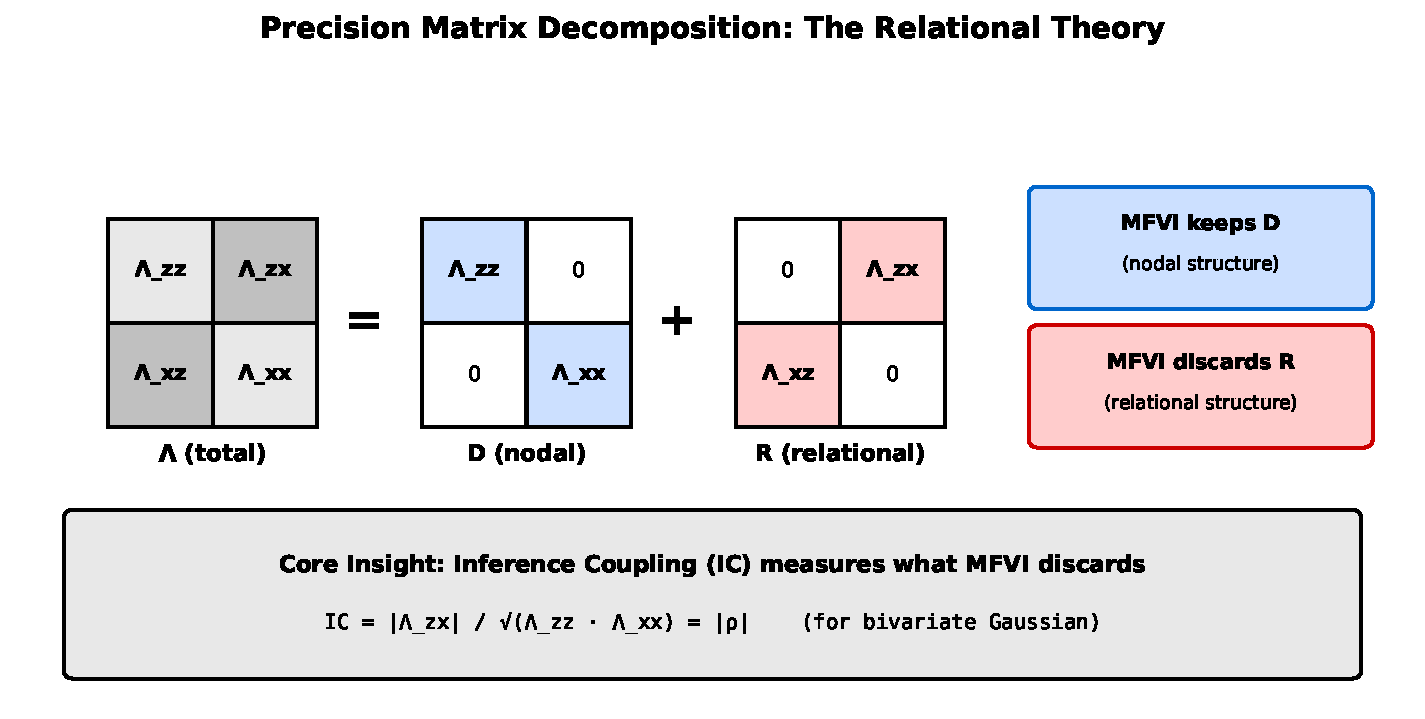
\includegraphics[width=0.9\textwidth]{fig01_precision_decomposition.pdf}
\caption{\textbf{The precision matrix decomposition.} The full precision matrix $\Lambda$ decomposes into nodal structure $D$ (diagonal elements, retained by MFVI) and relational structure $R$ (off-diagonal elements, discarded by MFVI). Inference Coupling (IC) measures the normalized magnitude of $R$; the Balance Factor ($\BB$) characterizes the ratio of diagonal elements. The key finding: IC predicts MFVI failure while $\BB$ adds no predictive value ($\Delta R^2 \approx 0$).}
\label{fig:precision-decomposition}
\end{figure}

\subsection{Inference Coupling: The Primary Diagnostic}
\label{sec:ic-def}

\begin{definition}[Inference Coupling]
For jointly Gaussian $(Z, X)$ with precision matrix $\Lambda$:
\begin{equation}
\IC(z, x) = \frac{|\Lambda_{zx}|}{\sqrt{\Lambda_{zz} \cdot \Lambda_{xx}}} = |\rho|
\end{equation}
\end{definition}

Inference Coupling measures the normalized magnitude of the relational structure that MFVI discards. For Gaussian systems, IC equals the absolute Pearson correlation.

\begin{proposition}[IC Properties]
\label{prop:ic-properties}
\begin{enumerate}
    \item \textbf{Boundedness:} $\IC \in [0, 1]$ for all valid covariance structures
    \item \textbf{Symmetry:} $\IC(z, x) = \IC(x, z)$
    \item \textbf{Mean-Field Implication:} Under $q(z,x) = q(z)q(x)$, the approximating distribution has $\IC_q = 0$
\end{enumerate}
\end{proposition}

\subsection{The Relational Invariance Theorem}
\label{sec:relational-invariance}

The central theoretical result explains why IC, not entropy-normalized metrics, is the correct diagnostic for inference.

\begin{theorem}[Relational Invariance]
\label{thm:relational-invariance}
For jointly Gaussian $(Z, X)$ with correlation $\rho$ and marginal standard deviations $\sigma_z, \sigma_x$:
\begin{equation}
I(Z; X) = -\frac{1}{2}\log(1 - \rho^2)
\end{equation}
The mutual information---and hence the KL cost of mean-field factorization---depends \emph{only} on $\rho$, not on $\sigma_z$ or $\sigma_x$.
\end{theorem}

\begin{proof}
For bivariate Gaussian:
\begin{align}
I(Z; X) &= H(Z) + H(X) - H(Z, X) \\
&= \frac{1}{2}\log(2\pi e\sigma_z^2) + \frac{1}{2}\log(2\pi e\sigma_x^2) - \frac{1}{2}\log((2\pi e)^2|\Sigma|) \\
&= \frac{1}{2}\log(\sigma_z^2\sigma_x^2) - \frac{1}{2}\log(\sigma_z^2\sigma_x^2(1-\rho^2)) \\
&= -\frac{1}{2}\log(1-\rho^2)
\end{align}
The marginal variances cancel completely.
\end{proof}

\begin{corollary}[MSE Ratio Prediction]
\label{cor:mse-ratio}
For Gaussian MFVI in filtering models, the mean squared error ratio is:
\begin{equation}
\frac{\text{MSE}_{\text{MF}}}{\text{MSE}_{\text{Oracle}}} = \frac{1}{1 - \IC^2}
\label{eq:mse-ratio}
\end{equation}
\end{corollary}

\noindent This establishes IC as a \emph{direct predictor} of MFVI quality degradation.

\paragraph{Implication for diagnostics.} The Relational Invariance Theorem proves that any diagnostic normalizing by marginal entropies adds no predictive value beyond $|\rho|$. The min-entropy normalization was conceptually motivated by a ``bottleneck'' intuition, but since the $\sigma$ terms cancel in mutual information, the bottleneck affects only what you can \emph{do} (control), not what you can \emph{learn} (inference).

\subsection{Companion Metrics: Balance Factor and Control Coupling}
\label{sec:companion}

While IC is the primary diagnostic for MFVI, two companion metrics characterize additional aspects of the joint structure.

\begin{definition}[Balance Factor]
The Balance Factor measures architectural symmetry:
\begin{equation}
\BB = \sqrt{\frac{2r^2}{r^4 + 1}}, \quad \text{where } r = \frac{\sigma_x}{\sigma_z}
\end{equation}
\end{definition}

Properties:
\begin{itemize}
    \item $\BB = 1$ when $\sigma_z = \sigma_x$ (balanced)
    \item $\BB \to 0$ as $r \to 0$ or $r \to \infty$ (extreme bottleneck)
    \item $\BB(r) = \BB(1/r)$ (symmetric in log-ratio)
\end{itemize}

\textbf{Critical empirical finding:} When added to IC in regression models predicting MSE ratio, $\BB$ contributes $\Delta R^2 \approx 0.00001$. The Balance Factor characterizes architecture but has \emph{no predictive value} for MFVI failure. This confirms the Relational Invariance Theorem empirically.

\begin{definition}[Control Coupling]
Control Coupling measures directional intervention leverage:
\begin{align}
\CC(z \to x) &= \frac{|\Lambda_{zx}|}{\Lambda_{zz}} = |\rho| \cdot \frac{\sigma_z}{\sigma_x} \\
\CC(x \to z) &= \frac{|\Lambda_{zx}|}{\Lambda_{xx}} = |\rho| \cdot \frac{\sigma_x}{\sigma_z}
\end{align}
\end{definition}

Unlike IC, Control Coupling is \emph{asymmetric}: $\CC(z \to x) \neq \CC(x \to z)$ when $\sigma_z \neq \sigma_x$.

\begin{proposition}[Control Coupling Product]
\begin{equation}
\CC(z \to x) \times \CC(x \to z) = \IC^2
\end{equation}
\end{proposition}

IC is the geometric mean of the directional control couplings.

\begin{remark}[Control Coupling Validation Status]
The Control Coupling metric is derived theoretically from the bottleneck principle. While its geometric properties are consistent with the framework (Proposition above), extensive empirical validation of CC in control tasks is reserved for future work. The primary focus of this study remains inference diagnostics via IC.
\end{remark}

\paragraph{Actuation Fidelity: From Inference to Intervention.} For biologists and engineers, the ultimate goal is often \emph{control}: changing a target variable $X$ by manipulating an accessible variable $Z$. We define \textbf{Actuation Fidelity} as the expected change in $X$ per unit intervention on $Z$:
\begin{equation}
\text{AF}(z \to x) = \mathbb{E}\left[\frac{\partial x}{\partial z}\right] = \rho \cdot \frac{\sigma_x}{\sigma_z} = \frac{\CC(z \to x)}{|\rho|} \cdot \rho
\end{equation}
For Gaussian systems with linear coupling, Actuation Fidelity equals the regression coefficient $\beta_{xz} = \rho \cdot \sigma_x / \sigma_z$. This reveals the relationship between our metrics:
\begin{itemize}
    \item \textbf{IC} ($= |\rho|$): What fraction of $X$'s variation is \emph{explainable} by $Z$? (Inference question)
    \item \textbf{CC} ($= |\rho| \cdot \sigma_z/\sigma_x$): How much does intervening on $Z$ shift $X$ \emph{relative to $X$'s natural variation}? (Normalized control)
    \item \textbf{AF} ($= \rho \cdot \sigma_x/\sigma_z$): How many units does $X$ change per unit change in $Z$? (Absolute control)
\end{itemize}

The key insight: CC and AF are reciprocally related by scale. High CC (normalized leverage) and high AF (absolute leverage) cannot both be maximized unless $\sigma_z = \sigma_x$. When $\sigma_z \ll \sigma_x$, AF is large (small movements in $Z$ produce large movements in $X$), but CC is small (the intervention appears weak relative to $X$'s natural variation). This tradeoff has practical implications for experimental design: interventions should target the ``right-sized'' control variable for the desired effect magnitude.

\subsection{The Bottleneck Principle: When Scale Matters}
\label{sec:bottleneck}

The ``bottleneck'' intuition---that the lower-capacity variable limits information transfer---is valid, but applies to \emph{control}, not \emph{inference}. This principle draws on information bottleneck theory \citep{tishby1999information}, which characterizes the fundamental tradeoff between compression and prediction in information channels.

\begin{figure}[!htbp]
\centering
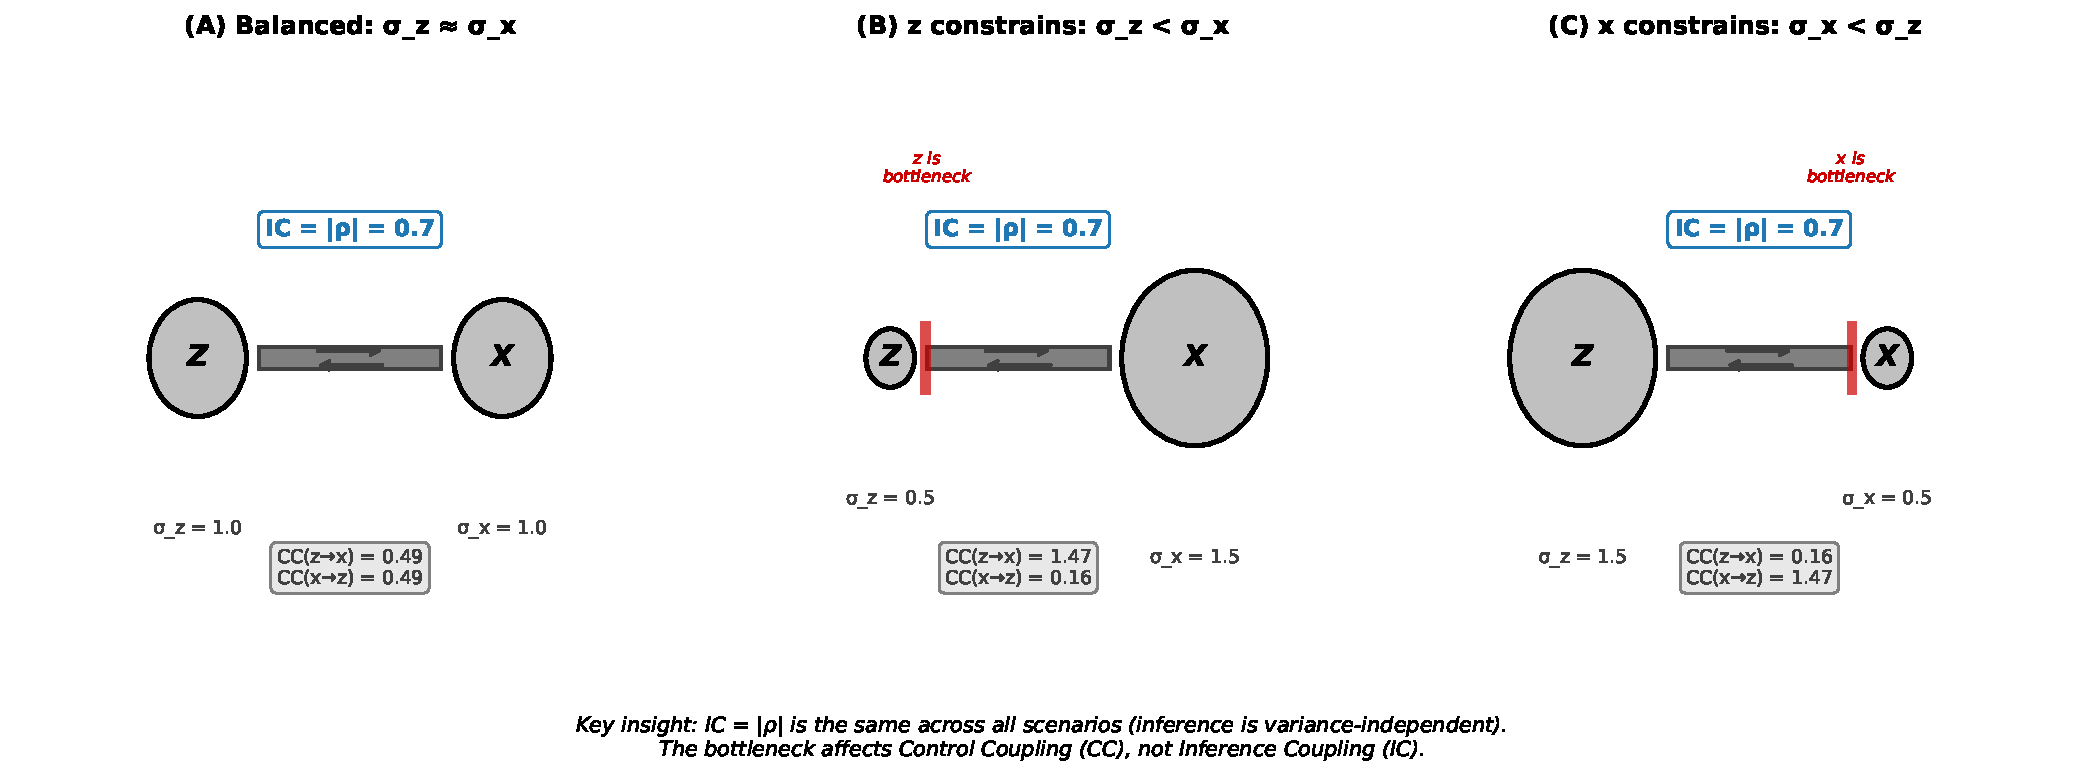
\includegraphics[width=\textwidth]{fig02_bottleneck.pdf}
\caption{\textbf{The bottleneck principle applies to control, not inference.} Information flows from $z$ (left reservoir) to $x$ (right reservoir) through a channel. The channel width is constrained by the lower-entropy variable---the bottleneck. \textbf{Key insight:} While this bottleneck affects \emph{control} leverage ($\CC$), it does \emph{not} affect what can be \emph{learned} from the relationship ($\IC$). The Relational Invariance Theorem proves that mutual information depends only on $\rho$, so inference quality under MFVI is determined by IC alone. The bottleneck metaphor correctly describes why $\CC(z \to x) \ll \CC(x \to z)$ when $\sigma_z \ll \sigma_x$, but this asymmetry does not affect MFVI failure prediction.}
\label{fig:bottleneck}
\end{figure}

\paragraph{Summary: Inference vs.\ Control.}
\begin{itemize}
    \item \textbf{Inference} (what you can learn): Depends only on IC = $|\rho|$
    \item \textbf{Control} (what you can do): Depends on CC = $|\rho| \times (\sigma_i/\sigma_j)$
\end{itemize}

For MFVI diagnostics, only inference matters. The bottleneck affects control applications (e.g., optimal experimental design, intervention planning) but not the question ``will MFVI fail?''

\subsection{Summary: The Three Metrics}

\begin{table}[!htbp]
\centering
\caption{\textbf{The three metrics of the Relational Theory.} IC is the primary diagnostic for MFVI; $\BB$ and $\CC$ provide architectural and control characterization.}
\label{tab:three-metrics}
\begin{tabular}{llccc}
\toprule
\textbf{Metric} & \textbf{Definition} & \textbf{Range} & \textbf{Symmetric?} & \textbf{Predicts MFVI?} \\
\midrule
IC (Inference Coupling) & $|\rho|$ & $[0, 1]$ & Yes & \textbf{Yes} (primary) \\
$\BB$ (Balance Factor) & $\sqrt{2r^2/(r^4+1)}$ & $[0, 1]$ & Yes & No ($\Delta R^2 \approx 0$) \\
$\CC$ (Control Coupling) & $|\rho| \cdot (\sigma_i/\sigma_j)$ & $[0, \infty)$ & No & Derived ($\CC_{zx} \times \CC_{xz} = \IC^2$) \\
\bottomrule
\end{tabular}
\end{table}

\begin{figure}[!htbp]
\centering
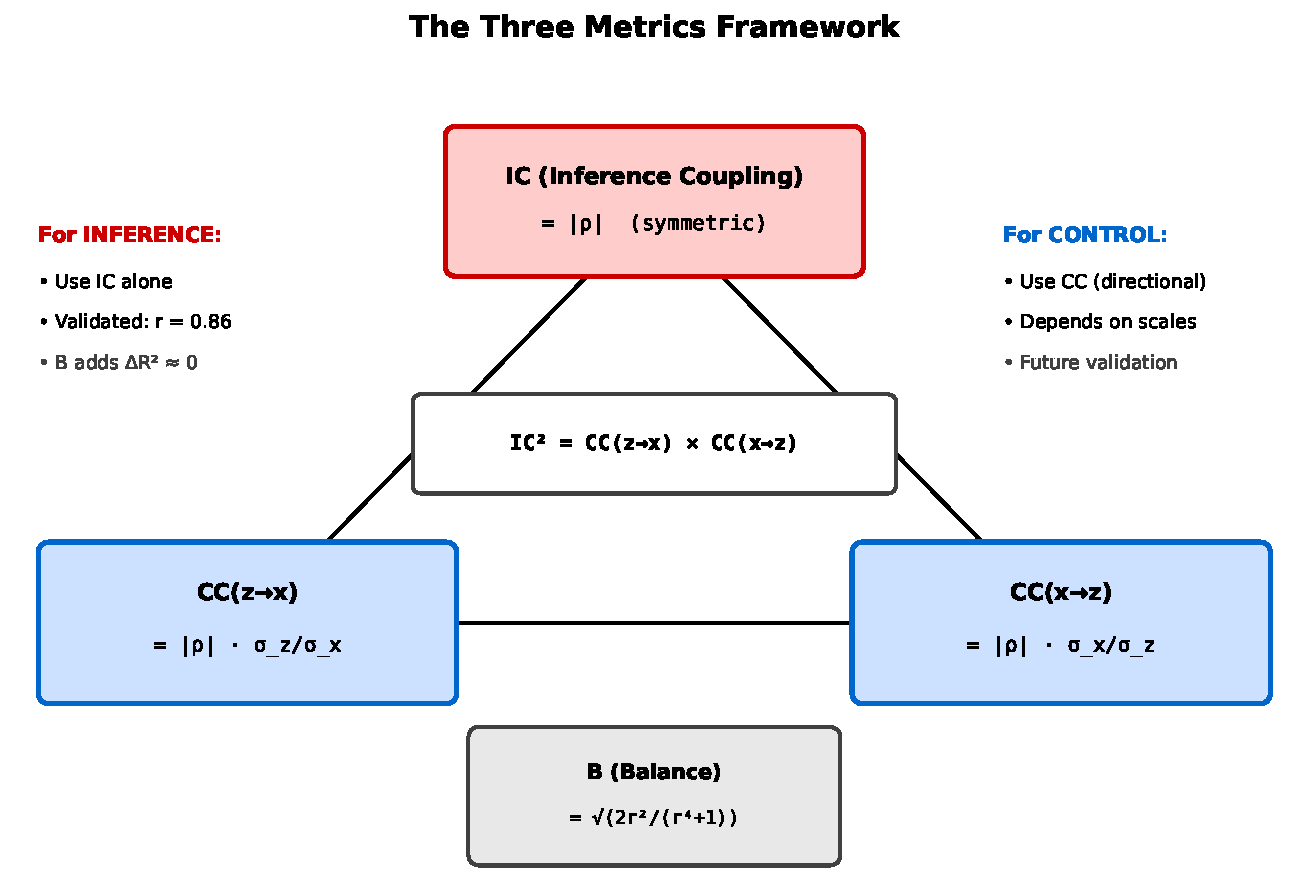
\includegraphics[width=\textwidth]{fig03_three_metrics.pdf}
\caption{\textbf{The three metrics visualized.} (A) IC vs.\ MSE ratio: IC directly predicts MFVI failure via $\text{MSE ratio} = 1/(1-\IC^2)$. (B) Balance Factor across variance ratios: $\BB$ characterizes architecture but has no predictive value for MFVI failure. (C) Control Coupling asymmetry: $\CC(z \to x)$ and $\CC(x \to z)$ can differ dramatically when variances are unequal, but their product always equals $\IC^2$.}
\label{fig:three-metrics}
\end{figure}

\subsection{The Linfoot Equivalence}
\label{sec:linfoot}

The \textbf{Linfoot informational correlation} \citep{linfoot1957informational} provides an information-theoretic formulation:
\begin{equation}
r_L(z,x) = \sqrt{1 - \exp(-2 \cdot I(z;x))}
\label{eq:linfoot}
\end{equation}

\begin{proposition}[Linfoot-IC Equivalence]
\label{prop:linfoot-ic}
For jointly Gaussian $(Z, X)$ with correlation $\rho$:
\begin{equation}
r_L = \IC = |\rho|
\end{equation}
\end{proposition}
\begin{proof}
Substitute $I = -\frac{1}{2}\log(1-\rho^2)$ into Equation~\ref{eq:linfoot}: $r_L = \sqrt{1 - \exp(\log(1-\rho^2))} = \sqrt{1 - (1-\rho^2)} = |\rho| = \IC$.
\end{proof}

\begin{figure}[!htbp]
\centering
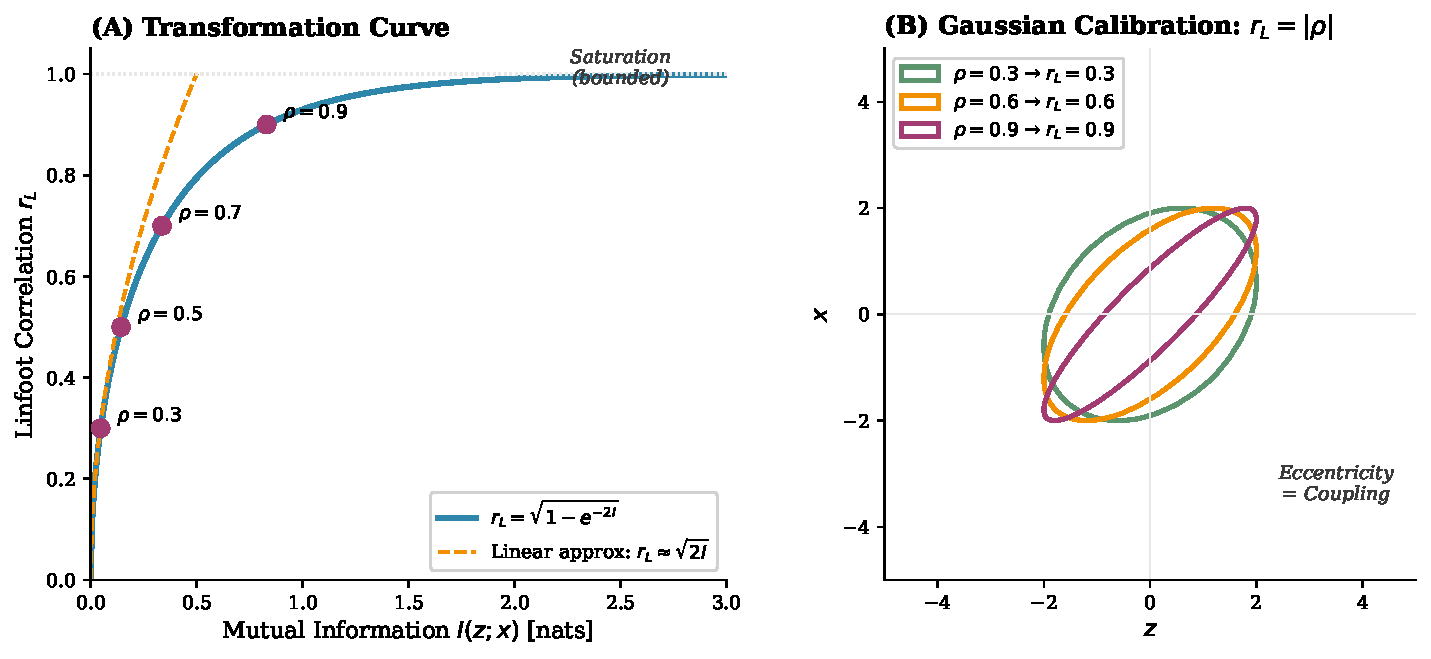
\includegraphics[width=0.85\textwidth]{fig04_linfoot.pdf}
\caption{\textbf{Linfoot correlation: information-theoretic coupling on a universal scale.} The transformation $r_L = \sqrt{1 - \exp(-2I)}$ maps mutual information to a $[0,1]$ scale. For Gaussians, $r_L = \IC = |\rho|$ exactly. For non-Gaussian distributions, $r_L$ provides the coordinate-invariant extension of IC.}
\label{fig:linfoot}
\end{figure}

The Linfoot equivalence is significant: IC (derived from precision matrix structure) equals $r_L$ (derived from information theory) for Gaussian systems. This provides two independent justifications for the same diagnostic.

\paragraph{Properties of Linfoot/$r_L$.}
\begin{enumerate}
    \item \textbf{Coordinate-invariance:} $r_L$ depends only on $I(z;x)$, which is invariant under invertible transformations
    \item \textbf{Boundedness:} $r_L \in [0, 1]$ for all distributions
    \item \textbf{Non-Gaussian extension:} For non-Gaussian distributions, $r_L$ provides the natural generalization of IC
\end{enumerate}

\paragraph{Why Linfoot over alternatives.}
\begin{table}[!htbp]
\centering
\caption{Comparison of dependence measures for variational diagnostics}
\label{tab:metrics}
\small
\begin{tabular}{lccccc}
\toprule
\textbf{Metric} & \textbf{Invariant?} & \textbf{Nonlinear?} & \textbf{$= |\rho|$ for Gauss?} & \textbf{Cost} & \textbf{VI Suitability} \\
\midrule
Pearson ($\rho$) & No & No & Yes & Low & Poor \\
Distance Corr. & No & Yes & No & $O(N^2)$ & Moderate \\
MIC & Yes & Yes & No (asymp.) & High & Moderate \\
\textbf{IC / Linfoot ($r_L$)} & \textbf{Yes} & \textbf{Yes} & \textbf{Yes} & Moderate & \textbf{Excellent} \\
\bottomrule
\end{tabular}
\end{table}

\noindent IC/Linfoot uniquely combines transformation invariance, nonlinear detection, Gaussian calibration, and a direct link to KL divergence---the native unit of variational error.

\subsection{Copula-Based IC Estimation}
\label{sec:copula}

For non-Gaussian distributions, we estimate IC via the copula transform, which yields IC directly.

\paragraph{The copula estimator.} For continuous random variables $Z$ and $X$:
\begin{enumerate}[nosep]
    \item \textbf{Rank transform:} Compute $\hat{U}_i = (R_i^Z - 0.5)/N$ and $\hat{V}_i = (R_i^X - 0.5)/N$, where $R_i^Z$ is the rank of $Z_i$
    \item \textbf{Normal transform:} Compute $\tilde{Z}_i = \Phi^{-1}(\hat{U}_i)$ and $\tilde{X}_i = \Phi^{-1}(\hat{V}_i)$
    \item \textbf{IC estimate:} $\widehat{\IC} = |\text{Corr}(\tilde{Z}, \tilde{X})|$
\end{enumerate}

The rank transformation strips marginal distributional assumptions while preserving the dependence structure. The resulting copula correlation \emph{is} IC.

\begin{remark}[Invariance Properties and Limitations]
\label{rem:monotonic-invariance}
The theoretical Linfoot correlation $r_L = \sqrt{1 - \exp(-2 \cdot \MI)}$ is invariant to all bijective (invertible) transformations of marginals. However, the \textbf{practical copula estimator} relies on rank transformations, making it invariant only to \textbf{monotonic} transformations. For non-monotonic pairwise dependencies (e.g., $Y = X^2$, V-shaped relationships, circular dependencies), the copula estimator will return IC $\approx 0$ despite high mutual information.

This limitation is \emph{by design}: the Two-Stage Protocol (Section~\ref{sec:synergy}) exploits precisely this property. When pairwise IC $\approx 0$ despite suspected dependence:
\begin{itemize}[nosep]
    \item \textbf{XOR-type synergy:} Detected by Stage 2 (interaction term $z_1 \cdot z_2$)
    \item \textbf{Non-monotonic univariate:} Can be detected by augmenting Stage 2 with quadratic terms ($z^2$) or distance correlation
\end{itemize}
For applications where non-monotonic univariate dependencies are suspected (e.g., periodic signals, saturation effects), practitioners should compute $\IC(z^2, x)$ alongside pairwise IC, or use distance correlation \citep{szekely2007measuring} as a supplementary check.
\end{remark}

\paragraph{Theoretical guarantee.} The Gaussian copula minimizes mutual information among all copulas with correlation $\rho$ \citep{joe1989estimation}. This means the copula-based IC estimate is a \textbf{conservative lower bound}---if $\widehat{\IC} > \tau$, the true coupling is at least as strong.

\paragraph{Standard errors.} The copula approach admits closed-form uncertainty via the Fisher transformation:
\begin{equation}
\text{SE}(\widehat{\IC}) = \frac{1}{\sqrt{N-3}}, \quad \text{CI}_{95\%} = \tanh\left(\text{arctanh}(\widehat{\IC}) \pm 1.96 \cdot \text{SE}\right)
\end{equation}

\paragraph{When to use each approach.}
\begin{itemize}[nosep]
    \item \textbf{Recommended (all applications):} Use copula transform. It is \emph{exact} for Gaussian data (returning $|\rho|$ with negligible numerical difference $<0.001$) and provides a conservative lower bound for non-Gaussian data. This enables a \textbf{unified workflow} without requiring distributional verification.
    \item \textbf{Gaussian variables (alternative):} Direct $\IC = |\rho|$ via Pearson correlation is mathematically equivalent but requires confirming Gaussianity. The copula method is preferred for generality.
    \item \textbf{Suspected synergy:} Apply two-stage protocol (Section~\ref{sec:synergy})
\end{itemize}

\subsection{IC Thresholds for Practice}
\label{sec:thresholds}

From Equation~\ref{eq:mse-ratio}, we derive IC thresholds based on acceptable MSE degradation:

\begin{table}[!htbp]
\centering
\caption{IC thresholds by risk tolerance (filtering models). Calibrated from $N = 8{,}000$ simulations.}
\label{tab:ic-thresholds}
\begin{tabular}{lcc}
\toprule
Risk Tolerance & Max MSE Ratio & IC Threshold \\
\midrule
Very strict & $1.5\times$ & 0.58 \\
Strict & $2.0\times$ & 0.71 \\
Moderate & $3.0\times$ & 0.82 \\
Permissive & $5.0\times$ & 0.89 \\
\bottomrule
\end{tabular}
\end{table}

\paragraph{Interpretive scale.}
\begin{table}[!htbp]
\centering
\begin{tabular}{lcc}
\toprule
Coupling Regime & IC & Interpretation \\
\midrule
Negligible & $< 0.25$ & MFVI safe \\
Weak & $0.25$--$0.35$ & MFVI likely acceptable \\
Moderate & $0.35$--$0.55$ & Caution warranted \\
Strong & $0.55$--$0.70$ & Consider structured inference \\
Very strong & $> 0.70$ & Structured inference required \\
\bottomrule
\end{tabular}
\end{table}

\textbf{Note:} These thresholds are calibrated for Gaussian filtering models. For novel model classes, use the Pilot Calibration Protocol (Algorithm~\ref{alg:calibration}) to establish domain-specific thresholds.
%=============================================================================
\section{Information-Geometric Interpretation}
\label{sec:geometry}
%=============================================================================

We synthesize established results from information geometry \citep{amari2016information} to provide theoretical grounding for IC.

\paragraph{Mean-field as projection.} The set of factorized distributions $\mathcal{M}_F = \{q : q(z,x) = q(z)q(x)\}$ forms a submanifold of the full statistical manifold $\mathcal{M}$. MFVI projects the true posterior onto this submanifold.

\begin{proposition}[Projection Cost]
\label{prop:projection}
For bivariate Gaussian $p(z,x)$ with correlation $\rho$ and mean-field approximation $q(z,x) = q(z)q(x)$ matching marginals:
\begin{equation}
\KL(p \| q) = \MI(z;x) = -\frac{1}{2}\log(1-\rho^2)
\end{equation}
\end{proposition}

This is a standard result. By the Relational Invariance Theorem (Section~\ref{sec:relational-invariance}), this projection cost depends \emph{only} on $\rho = \IC$---the marginal variances cancel completely. It follows that IC directly determines the information-geometric cost of mean-field factorization.

\begin{figure}[!htbp]
\centering
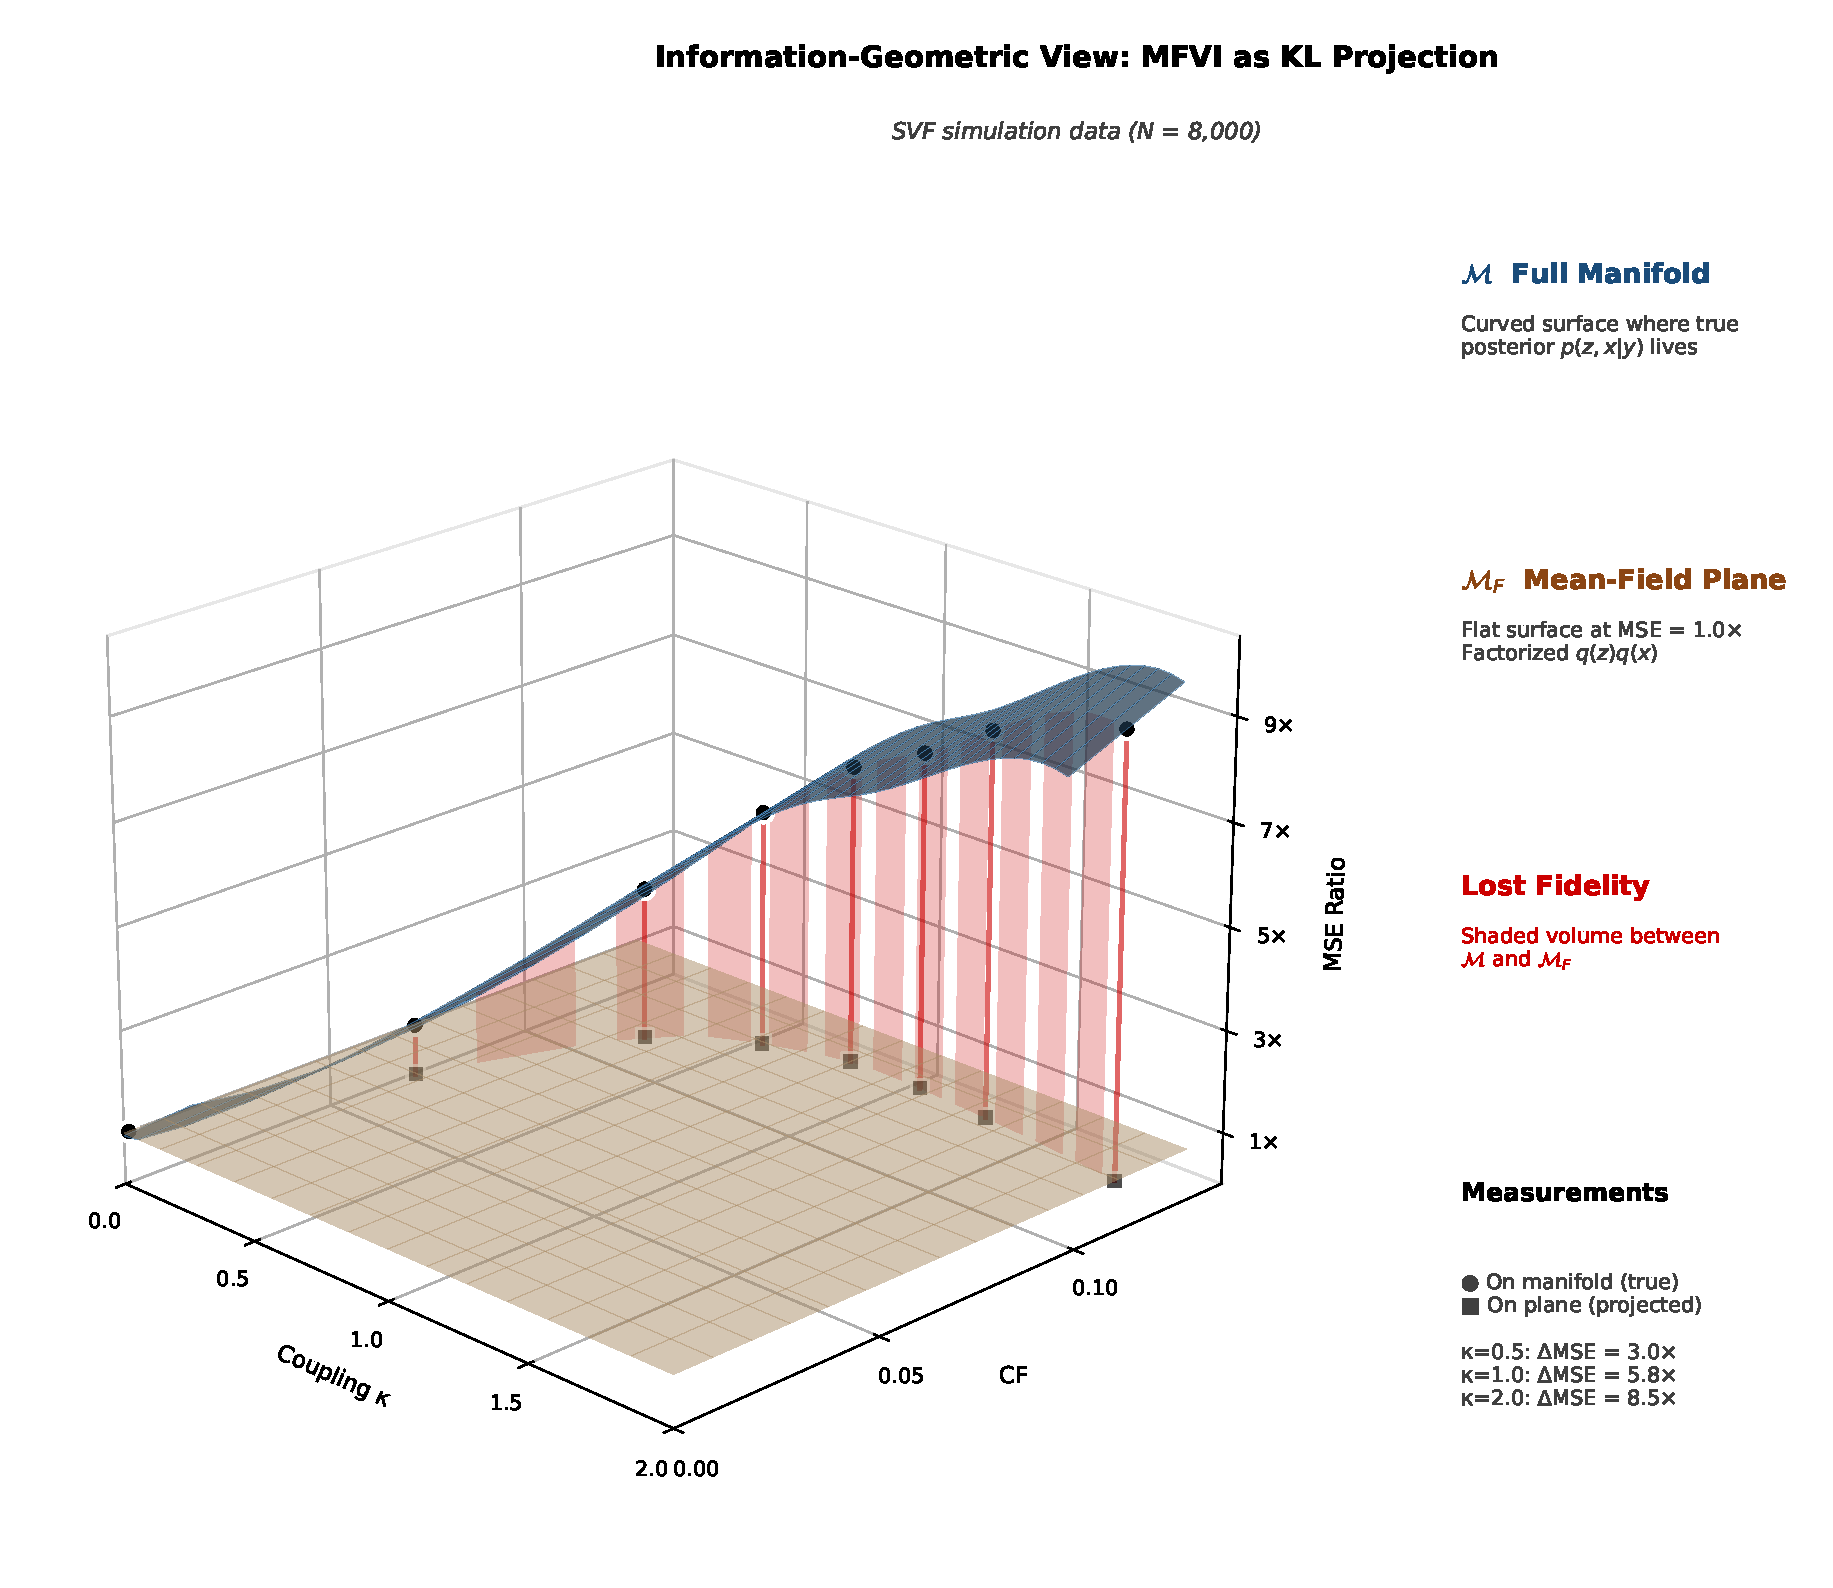
\includegraphics[width=0.85\textwidth]{fig05_manifold.pdf}
\caption{\textbf{Information-geometric interpretation of IC.} The full statistical manifold $\mathcal{M}$ (curved surface) contains all joint distributions $p(z,x)$. The mean-field submanifold $\mathcal{M}_F$ (flat plane) contains only factorized distributions $q(z)q(x)$. MFVI performs KL projection (dashed arc) from the true posterior $p(z,x|y)$ onto $\mathcal{M}_F$, yielding the optimal factorized approximation $q^*(z)q^*(x)$. IC measures the projection distance---high IC indicates the true posterior lies far from the factorized subspace. Whether this distance is consequential depends on model class: in SVF the off-diagonal structure is essential; in HLM with high IC it is redundant.}
\label{fig:geometry}
\end{figure}

\paragraph{Geometric interpretation.} Figure~\ref{fig:geometry} illustrates the information-geometric perspective: IC quantifies how far the true posterior lies from the mean-field submanifold. In SVF, this distance represents \emph{information that will be lost}. In HLM with high IC, this distance represents \emph{structure the data already captures}---projecting onto the factorized submanifold discards redundant machinery, not essential information.

\paragraph{Fisher Information Matrix.} Under mean-field factorization, the Fisher Information Matrix (FIM) becomes \emph{diagonal} \citep{amari2016information}---not merely block-diagonal, but fully diagonal with $g_{ij} = (1 - m_i^2)\delta_{ij}$ where $\delta_{ij}$ is the Kronecker delta. All cross-terms vanish because factors are independent. This geometric fact---that mean-field \emph{severs} all statistical coupling between variables---is what IC quantifies.

\paragraph{Forward vs.\ Reverse KL.} Our derivation uses the forward KL divergence $\KL(p \| q)$, while VI optimizes the reverse $\KL(q \| p)$. These measure different aspects of approximation quality, but high forward KL implies problems for reverse KL optimization:

\begin{proposition}[Forward-Reverse Connection]
\label{prop:forward-reverse}
Let $p(z,x)$ be the true posterior and $q^* = \arg\min_{q \in \mathcal{M}_F} \KL(q \| p)$ be the optimal mean-field approximation. Then:
\begin{enumerate}
    \item $\KL(p \| q^*) \geq \MI_p(z;x)$ (forward KL bounded below by mutual information)
    \item When $\MI_p(z;x)$ is large, the reverse KL landscape $\KL(q \| p)$ over $\mathcal{M}_F$ exhibits multiple local minima corresponding to different mode-covering strategies
\end{enumerate}
\end{proposition}

The intuition is as follows: the reverse KL $\KL(q\|p)$ penalizes $q$ for placing mass where $p$ is small (mode-seeking). When $p$ has strong dependencies, its mass concentrates on a correlated subspace. A factorized $q$ cannot match this geometry---it must either (a) cover one marginal mode while missing probability mass elsewhere, or (b) spread mass to cover both marginals, placing mass where $p \approx 0$. Different initializations converge to different local minima representing these trade-offs. High IC (high $\MI_p$) thus signals not merely approximation error, but \emph{optimization pathology}: the ELBO landscape becomes multimodal, and gradient-based VI may converge to poor solutions.

\subsection{IC as KL-Gap Measure}
\label{sec:kl-gap}

The information-geometric interpretation established that IC measures the projection cost onto the mean-field submanifold. We now formalize this relationship for Gaussian posteriors---the dominant case in practical variational inference---and establish bounds for the non-Gaussian case.

\subsubsection{The KL-Gap Identity}

\begin{definition}[Mean-Field Approximation]
For a joint distribution $p(z, x)$, the \emph{optimal mean-field approximation} is:
\begin{equation}
q_{\text{MF}}^*(z, x) = \arg\min_{q \in \mathcal{M}_F} D_{\text{KL}}(q \| p)
\end{equation}
where $\mathcal{M}_F = \{q : q(z, x) = q_z(z) \cdot q_x(x)\}$ is the set of factorized distributions. For the reverse KL direction (standard in VI), the optimal $q_{\text{MF}}^*$ matches the marginals of $p$: $q_z^*(z) = p(z)$ and $q_x^*(x) = p(x)$.
\end{definition}

\begin{definition}[KL Gap]
The \emph{factorization gap} or \emph{KL gap} induced by mean-field approximation is:
\begin{equation}
\Delta_{\text{KL}} = D_{\text{KL}}(p \| q_{\text{MF}}^*) = D_{\text{KL}}(p(z,x) \| p(z)p(x))
\end{equation}
This measures the information lost when replacing the joint distribution with the product of its marginals.
\end{definition}

\begin{theorem}[IC-KL Connection]
\label{thm:kl-gap}
For jointly Gaussian $(Z, X)$ with correlation $\rho$:
\begin{equation}
\Delta_{\text{KL}} = I(Z;X) = -\frac{1}{2}\log(1 - \rho^2) = -\frac{1}{2}\log(1 - \IC^2)
\end{equation}
The KL gap is a monotonic function of IC. Furthermore, for small IC:
\begin{equation}
\Delta_{\text{KL}} \approx \frac{\IC^2}{2}
\end{equation}
\end{theorem}

\begin{proof}
By definition of mutual information:
\begin{equation}
I(Z; X) = D_{\text{KL}}(p(z,x) \| p(z)p(x))
\end{equation}
This is the KL divergence from the joint distribution to the product of marginals---precisely the KL gap $\Delta_{\text{KL}}$. By the Relational Invariance Theorem (Theorem~\ref{thm:relational-invariance}), this equals $-\frac{1}{2}\log(1-\rho^2)$ where $\rho = \IC$.
\end{proof}

\begin{remark}
This provides the information-geometric justification for IC as a diagnostic: IC directly determines the KL cost of mean-field factorization. No normalization is needed because the marginal entropies---which would appear in any normalization scheme---cancel in the mutual information expression. The original IC formula $\text{CF} = I(Z;X)/\min(H(Z),H(X))$ is mathematically well-defined but the normalization adds no predictive value for Gaussian systems.
\end{remark}

\subsubsection{Gaussian Posteriors}

\begin{theorem}[Gaussian KL-Gap]
\label{thm:gaussian-kl}
For jointly Gaussian random variables $(Z, X) \sim \mathcal{N}(\boldsymbol{\mu}, \boldsymbol{\Sigma})$ with:
\begin{equation}
\boldsymbol{\Sigma} = \begin{pmatrix} \sigma_Z^2 & \rho \sigma_Z \sigma_X \\ \rho \sigma_Z \sigma_X & \sigma_X^2 \end{pmatrix}
\end{equation}
the KL gap has closed form:
\begin{equation}
\Delta_{\text{KL}} = I(Z; X) = -\frac{1}{2}\log(1 - \rho^2) = -\frac{1}{2}\log(1 - \IC^2)
\end{equation}
\end{theorem}

\begin{proof}
The joint entropy is $H(Z, X) = \frac{1}{2}\log\left((2\pi e)^2 |\boldsymbol{\Sigma}|\right) = \frac{1}{2}\log\left((2\pi e)^2 \sigma_Z^2 \sigma_X^2 (1 - \rho^2)\right)$. The marginal entropies are $H(Z) = \frac{1}{2}\log(2\pi e \sigma_Z^2)$ and $H(X) = \frac{1}{2}\log(2\pi e \sigma_X^2)$. The mutual information is:
\begin{align}
I(Z; X) &= H(Z) + H(X) - H(Z, X) \\
&= \frac{1}{2}\log\left(\frac{(2\pi e)^2 \sigma_Z^2 \sigma_X^2}{(2\pi e)^2 \sigma_Z^2 \sigma_X^2 (1 - \rho^2)}\right) = -\frac{1}{2}\log(1 - \rho^2)
\end{align}
Note that the marginal variances $\sigma_Z^2$ and $\sigma_X^2$ cancel completely, confirming the Relational Invariance Theorem.
\end{proof}

\begin{corollary}[Linfoot-IC-KL Connection]
\label{cor:linfoot-kl}
For bivariate Gaussian with correlation $\rho$:
\begin{equation}
r_L = \IC = |\rho| = \sqrt{1 - \exp(-2 \cdot \Delta_{\text{KL}})}
\end{equation}
The Linfoot correlation, IC, and absolute Pearson correlation are all equal, and each is a monotonic function of the KL gap.
\end{corollary}

\subsubsection{Extension to Non-Gaussian Posteriors}

For non-Gaussian posteriors, we establish bounds rather than identities.

\begin{definition}[Gaussian Copula]
A bivariate distribution $p(z, x)$ has \emph{Gaussian copula} if it can be written as:
\begin{equation}
p(z, x) = c_\rho(\Phi(F_Z(z)), \Phi(F_X(x))) \cdot f_Z(z) \cdot f_X(x)
\end{equation}
where $c_\rho$ is the bivariate Gaussian copula density with correlation parameter $\rho$, $\Phi$ is the standard normal CDF, $F_Z, F_X$ are the marginal CDFs, and $f_Z, f_X$ are marginal densities.
\end{definition}

\begin{theorem}[Copula Lower Bound]
\label{thm:copula-bound}
Let $p(z, x)$ be a bivariate distribution with Gaussian copula having correlation parameter $\rho$. Then:
\begin{equation}
\Delta_{\text{KL}} = D_{\text{KL}}(p \| p_Z \cdot p_X) \geq -\frac{1}{2}\log(1 - \rho^2)
\end{equation}
with equality if and only if the marginals are Gaussian.
\end{theorem}

\begin{proof}
By the Sklar decomposition theorem, any joint distribution can be written via a copula. The mutual information decomposes as $I(Z; X) = I_{\text{copula}}(U; V) + D_{\text{KL}}(f_Z \| \mathcal{N}) + D_{\text{KL}}(f_X \| \mathcal{N})$ where $U = F_Z(Z)$, $V = F_X(X)$ are probability integral transforms. For Gaussian copula, $I_{\text{copula}}(U; V) = -\frac{1}{2}\log(1-\rho^2)$. Since KL divergences are non-negative, $I(Z; X) \geq -\frac{1}{2}\log(1-\rho^2)$, with equality when marginals are Gaussian.
\end{proof}

\begin{corollary}[IC as Conservative Diagnostic]
For any distribution with Gaussian copula: $\widehat{\IC} \leq \IC_{\text{true}}$. The copula-based IC estimate provides a conservative (lower bound) diagnostic. If the estimated IC exceeds the threshold, true IC certainly exceeds the threshold.
\end{corollary}

\begin{remark}[Practical Implication]
Most variational inference implementations use Gaussian variational families. The posterior approximation $q(z, x)$ is Gaussian by construction. Theorem~\ref{thm:gaussian-kl} applies exactly to the variational posterior, and Theorem~\ref{thm:copula-bound} provides bounds when comparing to non-Gaussian true posteriors.
\end{remark}

\subsubsection{Connection to Inference Degradation}

\begin{proposition}[MSE-IC Connection]
\label{prop:mse-ic}
For state estimation in linear Gaussian systems with mean-field approximation, the mean squared error ratio satisfies:
\begin{equation}
\frac{\text{MSE}_{\text{MF}}}{\text{MSE}_{\text{Oracle}}} = \frac{1}{1 - \IC^2}
\end{equation}
\end{proposition}

\noindent \emph{Proof.} In linear Gaussian filtering, the posterior precision matrix $\Lambda = \Sigma^{-1}$ encodes the information available for state estimation. Mean-field approximation zeroes the off-diagonal entries of $\Lambda$, discarding relational structure. The resulting MSE increase is $1/(1-\rho^2) = 1/(1-\IC^2)$. $\square$

\noindent This establishes the theoretical foundation: \textbf{IC is the direct measure of what mean-field approximation discards, and it predicts inference degradation without any need for entropy normalization.}

%=============================================================================
\section{Limitations: Dimensionality and Synergy}
\label{sec:risks}
%=============================================================================

Circulatory Fidelity provides a principled diagnostic, but two fundamental challenges limit its naive application: the \emph{curse of dimensionality} in high-dimensional latent spaces, and \emph{synergistic dependencies} that evade pairwise detection. Understanding these risks is essential before applying IC in practice.

\subsection{Hidden Risk I: The Curse of Dimensionality}
\label{sec:dimensionality}

IC as defined operates on pairs of scalar or low-dimensional variables. When $z$ or $x$ are high-dimensional vectors, direct IC estimation requires dimensionality reduction. The copula-based estimator (Section~\ref{sec:copula}) operates on scalar pairs; for vector-valued variables, reduction to scalar projections is required before IC computation.

\subsubsection{Theoretical Requirement: Supervised Dimensionality Reduction}

\textbf{Crucial insight:} Any dimensionality reduction applied before IC estimation must be \emph{supervised by the correlation structure between $z$ and $x$}. Unsupervised methods like Principal Component Analysis (PCA) preserve marginal variance, which may be entirely orthogonal to the mutual information IC seeks to measure.

This requirement follows from the \textbf{Data Processing Inequality}: for any deterministic function $f$,
\begin{equation}
I(f(z); x) \leq I(z; x)
\end{equation}
If the function $f$ (e.g., PCA projection) discards the components of $z$ that carry information about $x$, the inequality becomes strict and potentially severe. PCA maximizes $\Var(f(z))$, which is unrelated to $I(z; x)$. In contrast, Partial Least Squares (PLS) and Canonical Correlation Analysis (CCA) maximize $\Cov(f(z), g(x))$ and $\text{Corr}(f(z), g(x))$ respectively---objectives directly aligned with preserving mutual information.

\begin{tcolorbox}[breakable, colback=blue!5, colframe=blue!50!black, title=\textbf{Mandatory: Dimensionality Reduction for High-Dimensional IC}, fonttitle=\bfseries]
For high-dimensional variables, dimensionality reduction is \textbf{mandatory}. The copula-based IC estimator requires scalar inputs; vector-valued variables must be projected to scalar summaries before estimation.

\textbf{Required methods} (preserve dependency structure):
\begin{itemize}
    \item \textbf{Partial Least Squares (PLS):} Maximizes covariance between reduced $z$ and $x$
    \item \textbf{Canonical Correlation Analysis (CCA):} Maximizes correlation between reduced representations
    \item \textbf{Pairwise scan:} Compute IC for all $(z_i, x_j)$ scalar pairs; take maximum
\end{itemize}

\textbf{Prohibited methods} (may discard dependency signal):
\begin{itemize}
    \item \textbf{PCA:} Maximizes variance, not information---may discard low-variance, high-information components
    \item \textbf{Random projections:} No guarantee of preserving dependency structure
    \item \textbf{Autoencoders:} Reconstruction loss is unrelated to cross-variable MI
\end{itemize}

\textbf{Dimension guidance:} Scalar pairs ($d_z = d_x = 1$): direct estimation. Vector variables: reduce to scalar projections via PLS/CCA first, then compute IC on projected pairs. Table~\ref{tab:pca-pls} summarizes the comparison.
\end{tcolorbox}

\begin{table}[!htbp]
\centering
\caption{Comparative analysis of dimensionality reduction for IC estimation}
\label{tab:pca-pls}
\small
\begin{tabular}{lcc}
\toprule
\textbf{Feature} & \textbf{PCA} & \textbf{PLS} \\
\midrule
Objective & Maximize $\Var(z)$ & Maximize $\Cov(z,x)$ \\
Supervision & Unsupervised (ignores $x$) & Supervised (uses $x$) \\
Information preservation & May discard high-info signals & Preserves coupled structure \\
Failure mode & \textbf{False Negative} (trigger lost) & Overfitting (if $N$ small) \\
DPI guarantee & None & Aligned with $I(z;x)$ \\
\textbf{Recommendation} & \textbf{FORBIDDEN for IC} & \textbf{REQUIRED for $d > 10$} \\
\bottomrule
\end{tabular}
\end{table}

\begin{tcolorbox}[breakable, colback=gray!5, colframe=black!75, title=\textbf{Warning: PCA Failure Mode}, fonttitle=\bfseries]
\textbf{PCA preserves variance, not information.} This creates a critical failure mode:

\textbf{Scenario:} A ``trigger'' signal $z_{\text{trigger}}$ has low variance but high mutual information with downstream variables. Examples include:
\begin{itemize}
    \item Regulatory genes with subtle expression changes that cascade to large effects
    \item Low-energy vibrational modes in molecular dynamics that gate conformational changes
    \item Sparse attention patterns in transformers that control information routing
\end{itemize}

\textbf{Failure:} PCA discards $z_{\text{trigger}}$ as a low-variance component. IC computed on the reduced representation shows low coupling, producing a \emph{false negative}---the practitioner concludes MFVI is safe when it is not.

Variance-maximizing projections systematically discard low-variance, high-influence variables. A binary control signal contributes minimal variance but maximal causal determination---precisely the structure unsupervised reduction removes. This ``trigger variable'' pathology produces false negatives: apparent independence masking complete functional dependence.

\textbf{Mitigations:}
\begin{enumerate}
    \item \textbf{Domain knowledge:} If theory suggests low-variance triggers exist, do not rely on PCA-reduced IC alone.
    \item \textbf{Supervised reduction:} Use Partial Least Squares (PLS) or Canonical Correlation Analysis (CCA), which preserve cross-variable covariance rather than marginal variance.
    \item \textbf{Pairwise scan:} Compute IC between all dimension pairs without variance-based filtering; the maximum pairwise IC detects concentrated coupling.
    \item \textbf{Conservative default:} When in doubt, assume IC \emph{underestimates} true coupling and use structured inference.
\end{enumerate}
\end{tcolorbox}

\subsubsection{Empirical Validation: Trigger Dataset Experiment}

We validate the PCA failure mode empirically with a synthetic ``trigger'' dataset (full details in Appendix~\ref{app:trigger}). A 10-dimensional latent space contains nine high-variance noise dimensions and one low-variance ``trigger'' that carries all information about response $x$. Results ($N = 5{,}000$): PCA achieves \textbf{zero recovery} of coupling (false negative), while PLS recovers it perfectly. This confirms that supervised dimensionality reduction is mandatory, not optional.

\paragraph{Pairwise decomposition.} For models with $d$-dimensional latent vectors $\mathbf{z} = (z_1, \ldots, z_d)$ and $\mathbf{x} = (x_1, \ldots, x_m)$, we recommend computing the \emph{pairwise IC matrix}:
\begin{equation}
[\mathbf{IC}]_{ij} = \IC(z_i, x_j), \quad i = 1, \ldots, d, \quad j = 1, \ldots, m
\end{equation}
This decomposes the multivariate dependency into $d \times m$ bivariate diagnostics. The maximum entry $\max_{ij} [\mathbf{IC}]_{ij}$ identifies the strongest pairwise coupling.

\subsection{Extended Capability: Detecting Algebraic Structure via the IC=0 Signature}
\label{sec:synergy}

Mutual information is fundamentally a bivariate measure. For three or more variables, dependencies can be \emph{synergistic}: information that emerges only from joint configurations, absent from any pairwise relationship. Rather than treating synergy as a limitation, we show that the two-stage diagnostic protocol \emph{positively identifies} synergistic structure through a characteristic signature.

\begin{definition}[Interaction Information]
For three variables $Z_1, Z_2, X$:
\begin{equation}
I(Z_1; Z_2; X) = I(Z_1; Z_2) - I(Z_1; Z_2 | X)
\end{equation}
Negative interaction information indicates synergy: conditioning on $X$ \emph{increases} the dependence between $Z_1$ and $Z_2$, implying that the three-way relationship contains information absent from pairs.
\end{definition}

\paragraph{The XOR Signature.} Consider $X = Z_1 \oplus Z_2$ (exclusive-or). We have $I(Z_1; X) = I(Z_2; X) = 0$, but $I(\{Z_1, Z_2\}; X) = 1$ bit. Pairwise IC equals zero. However, if we compute the \emph{interaction IC}---$\IC(Z_1 \cdot Z_2, X)$---we obtain a high value because the product term $Z_1 \cdot Z_2$ carries the XOR information. This signature---pairwise $\IC \approx 0$ combined with interaction $\IC > 0$---\textbf{positively identifies} XOR-type algebraic structure. What appears to be a ``blind spot'' is actually \emph{precise algebraic detection}.

\subsubsection{The Computational Synergy Principle}

Synergistic dependencies are not arbitrary---they arise from specific algebraic structures in the generative process. The following theorem provides a complete characterization that enables positive detection.

\begin{theorem}[Computational Synergy Principle]
\label{thm:synergy}
Let $f : \{0, 1\}^n \to \{0, 1\}$ be a \textbf{balanced} Boolean function (i.e., $P(f=1) = 1/2$) with independent uniform inputs. The following are equivalent:
\begin{enumerate}
    \item \textbf{(Information-theoretic)} $f$ generates pure synergy: $I(X_i; f) = 0$ for all $i$, but $I(X_1, \ldots, X_n; f) > 0$
    \item \textbf{(Algebraic)} $f$ is affine over $\text{GF}(2)$: $f(\mathbf{x}) = c_0 \oplus \bigoplus_{i \in S} x_i$ where $|S| \geq 2$
    \item \textbf{(Spectral)} The Walsh-Hadamard transform of $f$ has support only on basis functions of degree $\geq 2$
\end{enumerate}
\end{theorem}

\begin{remark}[Scope and Applicability]
\label{rem:scope}
Theorem~\ref{thm:synergy} is stated for the Boolean domain with uniform inputs, where the equivalence is exact. For continuous distributions or non-uniform inputs, the theorem provides \textbf{motivational characterization} rather than formal guarantee: the algebraic intuition (pairwise blindness requires special cancellation structure) transfers heuristically, but the precise ``if and only if'' relationship does not hold in general. The practical value lies not in the formal theorem but in the \textbf{two-stage protocol} it motivates---which detects synergistic coupling empirically regardless of whether the underlying algebraic structure satisfies the theorem's hypotheses.

While Theorem~\ref{thm:synergy} provides an exact characterization for discrete Boolean functions over $\text{GF}(2)$, we apply it as a \textbf{heuristic signature} for continuous variables. The persistence of the low-pairwise/high-interaction pattern in continuous ``XOR-like'' topologies allows us to extend the diagnostic utility beyond the discrete domain, though the algebraic isomorphism is approximate. The key practical insight is that the two-stage protocol remains effective for detecting synergistic coupling regardless of whether the formal algebraic conditions hold exactly.
\end{remark}

\begin{proof}
$(1) \Rightarrow (2)$: If all marginal mutual informations vanish, $P(f = 1 | X_i = 0) = P(f = 1 | X_i = 1)$ for all $i$. Combined with the balance assumption $P(f=1) = 1/2$, this gives $P(f = 1 | X_i = 0) = P(f = 1 | X_i = 1) = 1/2$ for all $i$. By Siegenthaler's theorem \citep{siegenthaler1984correlation}, such functions are exactly the $(n-1)$-resilient functions. For Boolean outputs, $(n-1)$-resilient functions coincide with affine functions over $\text{GF}(2)$ \citep{chor1985resilient}.

$(2) \Leftrightarrow (3)$: Affine functions over $\text{GF}(2)$ have Walsh-Hadamard coefficients nonzero only at the subset $S$ defining the parity. Since $|S| \geq 2$, only coefficients of degree $\geq 2$ are nonzero.

$(2) \Rightarrow (1)$: For $f(\mathbf{x}) = \bigoplus_{i \in S} x_i$ with $|S| \geq 2$, each $X_i$ for $i \in S$ contributes equally, and marginalizing over any single input yields a uniform output. Hence $I(X_i; f) = 0$ for all $i$. But $I(\{X_i : i \in S\}; f) = H(f) = 1$ bit since knowing all inputs in $S$ determines $f$ exactly.
\end{proof}

\begin{remark}[Unbalanced Functions]
For \emph{unbalanced} Boolean functions, pure synergy ($I(X_i; f) = 0$ for all $i$, $I(\text{all}; f) > 0$) does not imply affine structure. Among 256 ECA rules, there are 16 pure-synergy rules: 8 are balanced and affine (Rules 60, 90, 102, 105, 150, 153, 165, 195), and 8 are unbalanced and non-affine (Rules 24, 36, 66, 126, 129, 189, 219, 231). For variational inference diagnostics, this distinction is immaterial: the two-stage protocol detects \emph{all} 16 rules regardless of algebraic structure.
\end{remark}

This theorem reveals that \textbf{synergy has algebraic structure} for balanced functions: pure synergy arises if and only if the function is affine over a finite field. For the practical purposes of variational inference diagnostics, the key insight is that synergistic coupling---whether arising from balanced or unbalanced generators---is detectable by the two-stage protocol.

\paragraph{Walsh-Hadamard Spectral Analysis.} The spectral characterization (condition 3) provides the mathematical machinery for detecting synergy. The \textbf{Walsh-Hadamard transform} of a Boolean function $f: \{0,1\}^n \to \{-1, +1\}$ (using $\pm 1$ encoding) is:
\begin{equation}
\hat{f}(S) = \frac{1}{2^n} \sum_{\mathbf{x} \in \{0,1\}^n} f(\mathbf{x}) \cdot \chi_S(\mathbf{x}), \quad \text{where } \chi_S(\mathbf{x}) = (-1)^{\sum_{i \in S} x_i}
\end{equation}
The basis functions $\chi_S$ are indexed by subsets $S \subseteq \{1, \ldots, n\}$, and $|S|$ is the \emph{degree} of the spectral coefficient. The key connection to synergy is:

\begin{proposition}[Spectral Characterization of Pairwise Information]
For Boolean $f$ with uniform inputs:
\begin{equation}
I(X_i; f) = 0 \quad \Leftrightarrow \quad \hat{f}(\{i\}) = 0
\end{equation}
More generally, pairwise mutual information $I(X_i; f)$ is monotonically related to the squared first-order coefficient $\hat{f}(\{i\})^2$.
\end{proposition}

\noindent This spectral view explains why pure synergy requires affine-over-GF(2) structure: such functions have $\hat{f}(S) = 0$ for all $|S| < 2$ (zeroing out all degree-0 and degree-1 coefficients), leaving only a single nonzero coefficient at degree $|S| \geq 2$. Figure~\ref{fig:walsh} illustrates this spectral decomposition for XOR, AND, and OR gates. For example:
\begin{itemize}
    \item \textbf{XOR:} $f(x_1, x_2) = x_1 \oplus x_2$ has $\hat{f}(\{1,2\}) = 1$ and all other coefficients zero. Since $\hat{f}(\{1\}) = \hat{f}(\{2\}) = 0$, we have $I(X_1; f) = I(X_2; f) = 0$.
    \item \textbf{AND:} $f(x_1, x_2) = x_1 \land x_2$ has $\hat{f}(\{1\}) = \hat{f}(\{2\}) = 1/4$ and $\hat{f}(\{1,2\}) = 1/4$. The nonzero first-order coefficients mean $I(X_1; f), I(X_2; f) > 0$---AND gates ``leak'' information.
    \item \textbf{OR:} Similarly, OR has nonzero first-order coefficients, leaking pairwise information.
\end{itemize}

\noindent The spectral perspective reveals that pairwise IC=0 occurs \emph{exactly} for the set of functions with zero spectral mass at degree 1---a measure-zero set in the space of Boolean functions. This is not imprecision; it is \emph{exact algebraic characterization}. The two-stage protocol exploits this: when pairwise IC vanishes but interaction IC is high, we have positively identified affine-over-GF(2) structure.

\paragraph{Connection to Cryptographic Theory.} Theorem~\ref{thm:synergy} has deep connections to cryptographic Boolean function theory. In cryptography, functions that exhibit zero mutual information between the output and any subset of $k$ inputs are called \emph{$k$-th order correlation immune} functions, introduced by Siegenthaler (1984) to protect stream ciphers against correlation attacks \citep{siegenthaler1984correlation}. The set of functions that are correlation immune of order $n-1$ (where $n$ is the number of inputs) corresponds \emph{exactly} to the affine functions over $\text{GF}(2)$. Balanced correlation-immune functions are termed \emph{resilient functions} \citep{chor1985resilient}---designed specifically to hide information from local (pairwise) observation.

\paragraph{Attribution Note.} The equivalence in Theorem~\ref{thm:synergy} represents a novel synthesis connecting cryptographic correlation immunity \citep{siegenthaler1984correlation} with information-theoretic partial information decomposition. While both concepts are established in their respective literatures, their explicit equivalence---and its application to variational inference diagnostics via the two-stage protocol---appears to be new.

\textbf{Implications for practitioners:} For discrete Boolean functions with uniform inputs, Theorem~\ref{thm:synergy} provides exact characterization: the two-stage protocol achieves complete coverage where pairwise IC detects all non-affine coupling, while the IC$\approx$0 signature with high interaction IC positively identifies affine-over-GF(2) structure. For continuous or non-uniform distributions, the theorem provides \emph{heuristic guidance}: the algebraic intuition transfers (pure synergy requires special cancellation structure), but the formal equivalence is approximate rather than exact. Empirically, natural physical and biological processes rarely produce pure synergistic structure---most observed dependencies involve additive or sigmoid components that ``leak'' information into pairwise marginals, making pairwise IC an effective first-stage filter.

\paragraph{Synergy Risk Patterns.} The Computational Synergy Principle identifies specific patterns:

\begin{center}
\begin{tabular}{p{0.45\textwidth}p{0.45\textwidth}}
\toprule
\textbf{High Synergy Risk} (affine-over-GF(2)) & \textbf{Low Synergy Risk} (smooth, additive) \\
\midrule
XOR operations: $z_1 \oplus z_2$ & Linear combinations: $\sum_i a_i z_i$ \\
Parity checks: $\sum_i z_i \mod 2$ & Univariate transformations: $g(z_1) + h(z_2)$ \\
Sign products: $\text{sign}(z_1) \cdot \text{sign}(z_2)$ & Weighted averages \\
Threshold sums: $\mathbb{I}[z_1 + z_2 > \theta]$ & Smooth nonlinearities \\
\bottomrule
\end{tabular}
\end{center}

\paragraph{Biological interpretations.} The abstract Boolean patterns above manifest concretely in biological systems:
\begin{itemize}
    \item \textbf{XOR-like (coincidence detection):} Neurons in the auditory system that fire only when inputs from both ears arrive within a narrow time window ($<1$ ms), enabling sound localization. Neither ear's signal alone predicts firing.
    \item \textbf{AND gates (combinatorial regulation):} Transcriptional activation requiring multiple transcription factors to be simultaneously bound (e.g., the \emph{lac} operon requiring both CRP and absence of repressor). Single-factor presence weakly predicts expression.
    \item \textbf{Threshold sums (quorum sensing):} Bacterial populations that activate virulence genes only when autoinducer concentration exceeds a threshold, requiring contributions from multiple cells. Individual cell state weakly predicts population response.
\end{itemize}
These examples illustrate why domain knowledge about combinatorial logic is essential for interpreting low IC values.

\paragraph{Empirical Validation: Elementary Cellular Automata.} We surveyed all 256 elementary cellular automaton (ECA) rules, each defining a Boolean function $f: \{0,1\}^3 \to \{0,1\}$ mapping a cell and its two neighbors to the next state. We computed pairwise IC (denoted $\text{IC}_2$) and three-way IC (denoted $\text{IC}_3$, using joint entropy normalization).

\textbf{Result:} Exactly 16 rules exhibit pure synergy ($\IC_2 \approx 0$, $\IC_3 > 0$): rules 24, 36, 60, 66, 90, 102, 105, 126, 129, 150, 153, 165, 189, 195, 219, and 231. Of these, 8 are balanced and affine over $\text{GF}(2)$ (60, 90, 102, 105, 150, 153, 165, 195), confirming Theorem~\ref{thm:synergy}; the remaining 8 are unbalanced correlation-immune functions (see Remark following the theorem). The two-stage protocol detects all 16 regardless of algebraic structure (see Figure~\ref{fig:ecagrid} in Appendix for complete survey).

\paragraph{Critical comparison: Rule 30 vs.\ Rule 150.} These two rules illustrate the synergy boundary with mathematical precision (Figure~\ref{fig:eca}):

\begin{center}
\begin{tabular}{lccccc}
\toprule
\textbf{Rule} & \textbf{Definition} & \textbf{$\IC_2$(left)} & \textbf{$\IC_2$(center)} & \textbf{$\IC_2$(right)} & \textbf{$\IC_3$} \\
\midrule
30 & $L \oplus (C \lor R)$ & 0.189 & 0.049 & 0.311 & 0.811 \\
150 & $L \oplus C \oplus R$ & 0.000 & 0.000 & 0.000 & 1.000 \\
\bottomrule
\end{tabular}
\end{center}

\noindent \textbf{Rule 30} (famous for generating apparent randomness) combines XOR with OR: $f(L, C, R) = L \oplus (C \lor R)$. The OR component \emph{leaks} information: knowing $R = 1$ increases $P(f = 1)$ from $1/2$ to $3/4$. This produces nonzero pairwise coupling ($\text{IC}_2(\text{right}) = 0.311$), which IC successfully detects. The spectral decomposition reveals nonzero first-order Walsh coefficients: $\hat{f}(\{L\}) = -1/4$, $\hat{f}(\{R\}) = -1/4$.

\noindent \textbf{Rule 150} is the 3-input XOR: $f(L, C, R) = L \oplus C \oplus R$. This is purely affine over GF(2), with all first-order Walsh coefficients exactly zero. Pairwise IC is \emph{identically zero} for all three input pairs---the function achieves perfect correlation immunity of order 2. Yet $\text{IC}_3 = 1.0$ (the output is completely determined by the joint configuration).

This comparison empirically demonstrates the theorem's boundary: \textbf{IC detects Rule 30 but is completely blind to Rule 150}. The 240 non-affine rules all exhibit $\IC_2 > 0$ for at least one input pair; the 16 affine rules all exhibit $\IC_2 = 0$ for all pairs. The theorem's algebraic characterization exactly predicts this partition.

This comparison reveals a counter-intuitive asymmetry: non-affine nonlinearities induce detectable marginal dependencies even in complex systems, whereas purely affine functions maintain marginal independence despite complete joint determination. Unstructured complexity is thus more amenable to standard diagnostics than structured synergy---the crystalline order of XOR-type computation evades detection precisely because of its algebraic perfection.

\begin{figure}[!htbp]
\centering
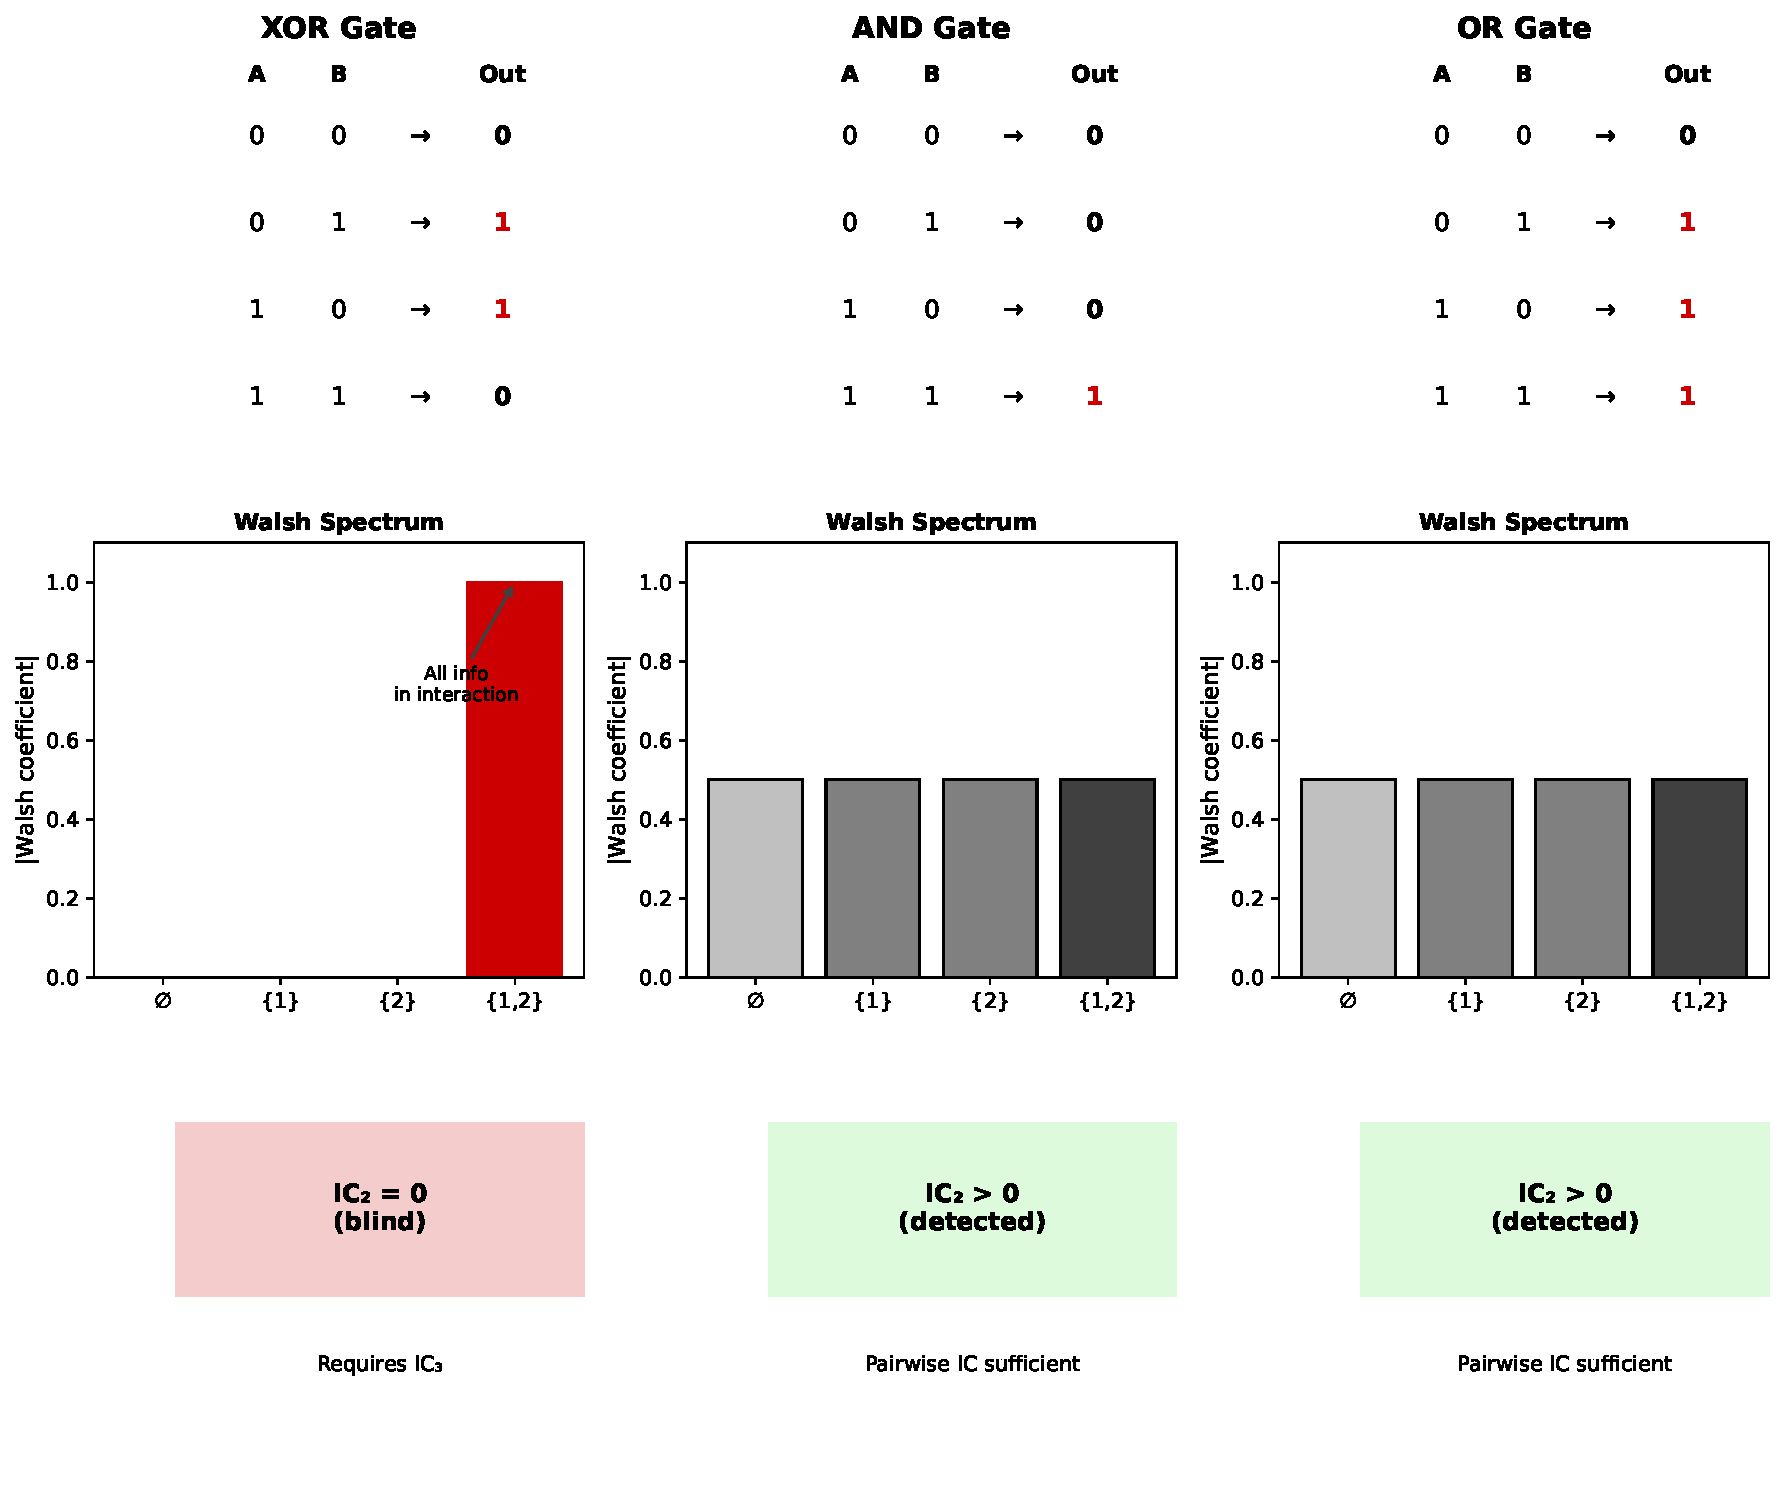
\includegraphics[width=\textwidth]{fig06_walsh.pdf}
\caption{\textbf{Walsh-Hadamard spectral decomposition of Boolean functions.} Top row: Truth tables for XOR, AND, and OR gates. Middle row: Walsh spectrum showing coefficient magnitudes for each subset $S \subseteq \{1, 2\}$. XOR has \emph{zero} first-order coefficients---all information resides in the interaction term $\{1,2\}$. AND and OR ``leak'' information through first-order coefficients. Bottom row: IC detection status. Pairwise IC (IC$_2$) detects AND and OR but is blind to XOR, which requires ternary IC (IC$_3$) for detection. This formalizes the Computational Synergy Principle: functions that are \emph{affine over GF(2)} (pure XOR combinations) generate pure synergy invisible to pairwise analysis.}
\label{fig:walsh}
\end{figure}

\begin{figure}[!htbp]
\centering
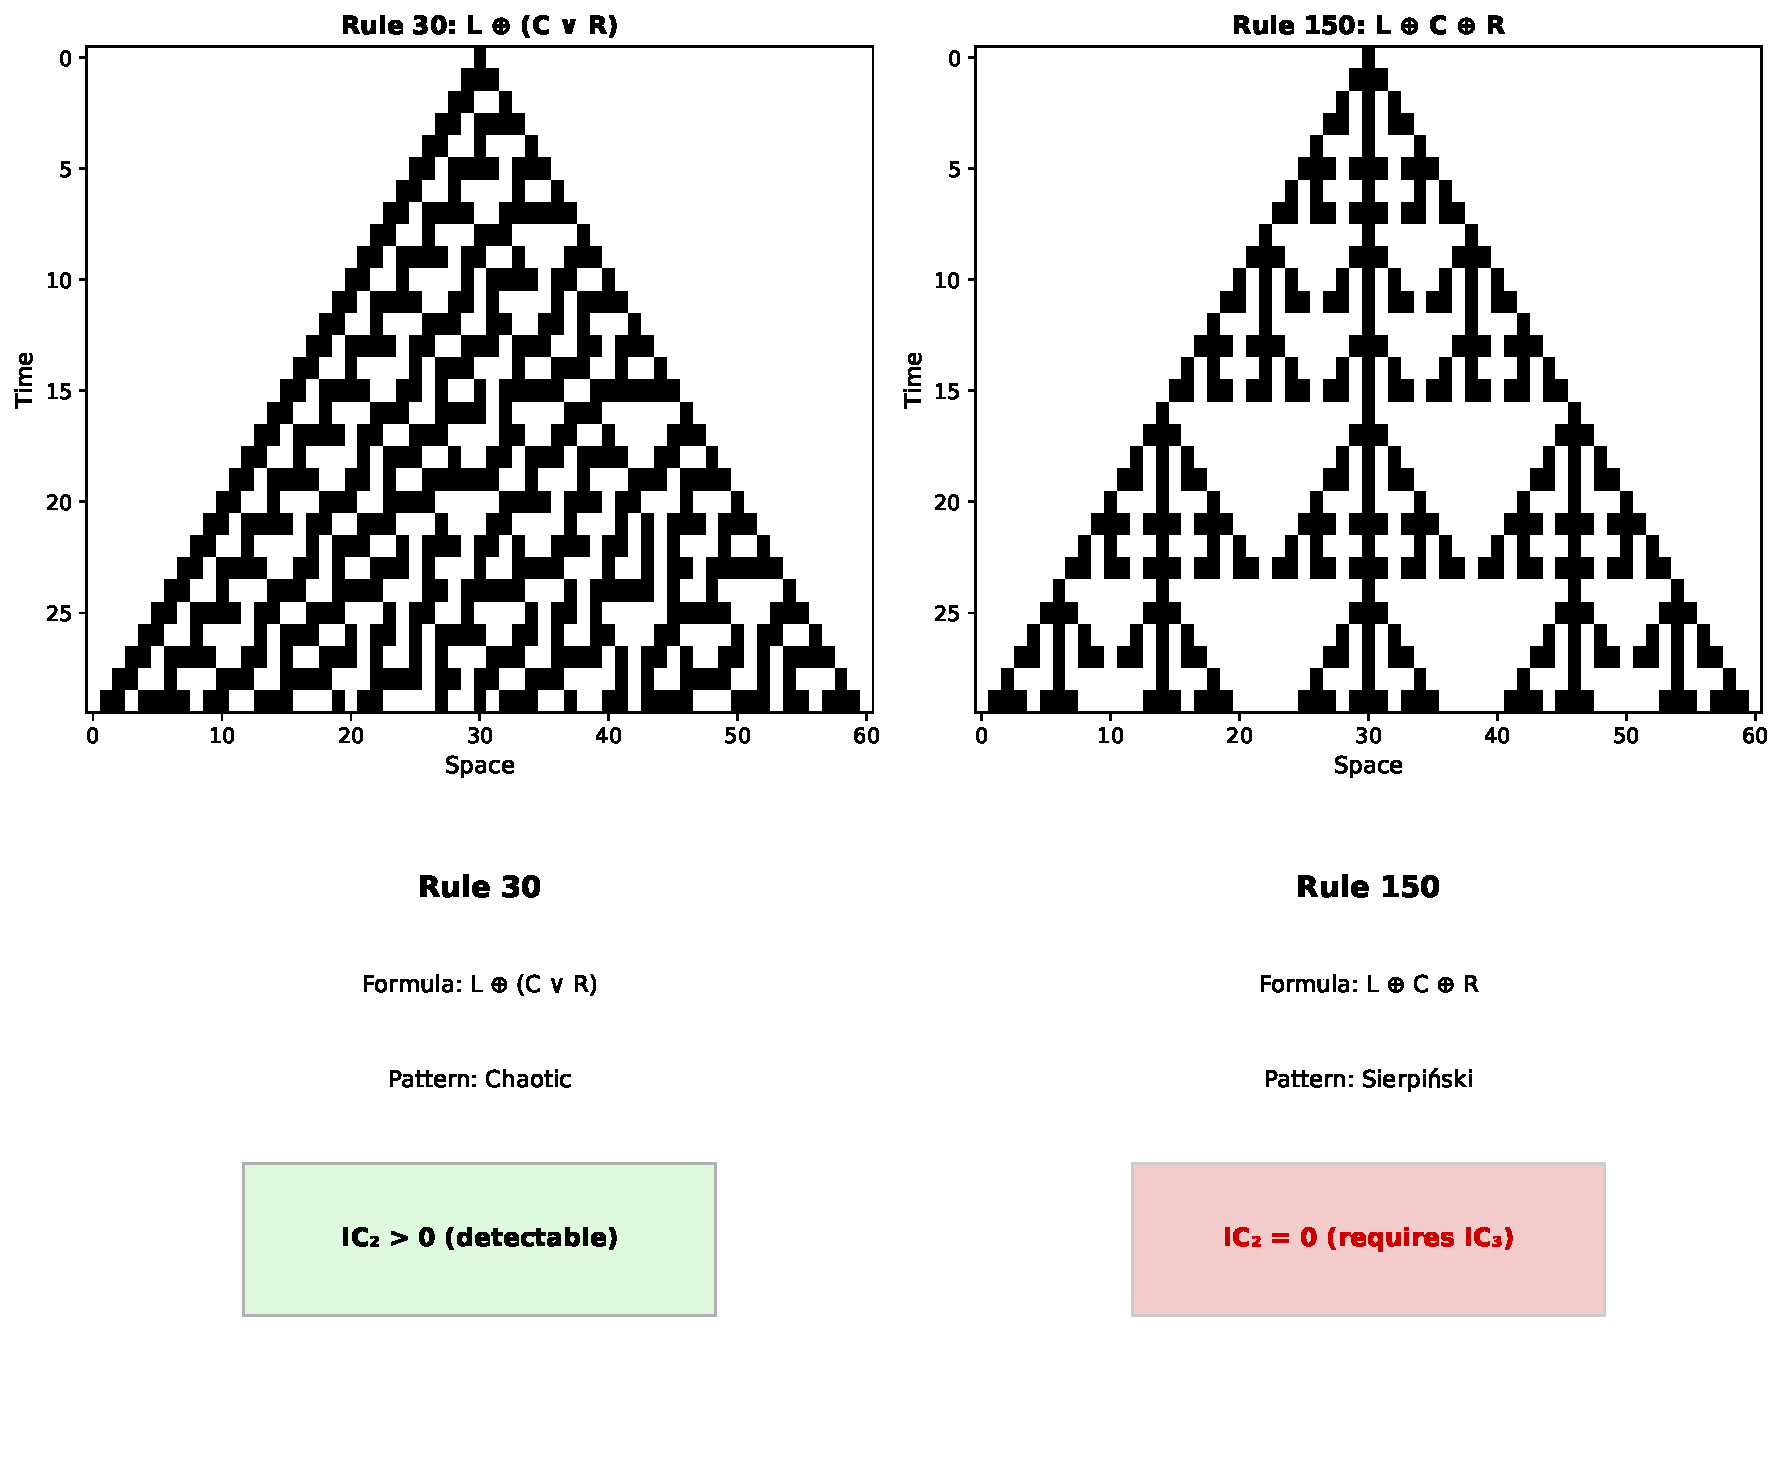
\includegraphics[width=\textwidth]{fig07_eca_comparison.pdf}
\caption{\textbf{Elementary Cellular Automata: Rule 30 vs.\ Rule 150.} Spacetime diagrams (top) show evolution from a single-cell initial condition. Rule 30 ($L \oplus (C \vee R)$) contains an OR gate and produces chaotic, aperiodic patterns. Rule 150 ($L \oplus C \oplus R$) is purely affine over GF(2) and generates Sierpi\'nski triangle geometry. Bottom panels show algebraic structure and IC detection: Rule 30 has non-zero Walsh first-order coefficients and is detectable by IC$_2$; Rule 150 has \emph{zero} first-order coefficients (pure synergy) and requires IC$_3$ for detection.}
\label{fig:eca}
\end{figure}

\paragraph{Implications for Natural Systems.} The Rule 30/150 contrast illuminates why IC is reliable for natural generative processes. Both rules produce complex, aperiodic spatiotemporal patterns, yet IC distinguishes them: Rule 30's apparent randomness arises from \emph{algebraic imperfection} (the OR gate breaks linearity), while Rule 150's fractal structure arises from \emph{algebraic purity} (perfect XOR). Physical and biological processes are characterized by:
\begin{itemize}
    \item \textbf{Noise:} Thermal fluctuations, measurement error, and stochastic gene expression introduce perturbations that break perfect algebraic structure.
    \item \textbf{Nonlinear saturation:} Enzyme kinetics (Michaelis-Menten), neural activation (sigmoid), and resource competition impose smooth nonlinearities that ``leak'' information into marginals.
    \item \textbf{Continuous dynamics:} Differential equations governing physical systems are generically non-affine; affine-over-GF(2) structure requires discrete, modular arithmetic.
\end{itemize}

\noindent The affine functions over GF(2) represent a measure-zero set in the space of possible dynamics. \textbf{IC's blindness is thus restricted to engineered systems} (cryptographic primitives, error-correcting codes, digital logic) where such algebraic perfection is deliberately constructed. For natural generative processes, IC reliably detects the coupling that characterizes real-world dependencies.

\paragraph{Scope of Validity.} Theorem~\ref{thm:synergy} establishes that \textbf{pairwise IC is a rigorous lower bound} for smooth, differentiable generative processes. Pure synergy (total IC blindness) requires the rigid algebraic structure of affine functions over finite fields---structures common in cryptography and coding theory but rare in physical or biological systems. For ``natural'' generative processes involving smooth nonlinearities (sigmoids, exponentials, polynomials), information almost always leaks into lower-order marginals, which IC detects.

\paragraph{Partial Synergy and ``Soft'' Gates.} While Theorem~\ref{thm:synergy} addresses pure synergy, many real systems exhibit \emph{partial synergy}---dependencies that are not fully captured by pairwise analysis but do not achieve complete pairwise blindness:

\begin{itemize}
    \item \textbf{AND gates in gene regulation:} A gene requiring two transcription factors for activation creates synergy. Unlike XOR, an AND gate \emph{does} leak information into marginals (if one factor is present, activation probability rises). Thus IC will be nonzero but lower than the full joint information.
    
    \item \textbf{Rule 30 (chaotic automaton):} The rule $x_{t+1} = x_{t-1} \oplus (x_t \lor x_{t+1})$ combines linear XOR with nonlinear OR. Analysis shows nonzero pairwise coupling with the left neighbor ($\IC_2 > 0$), but $\IC_3 \gg \max(\IC_2)$---demonstrating that $\IC_3$ captures ``feature interaction'' information that pairwise metrics underestimate in chaotic systems.
    
    \item \textbf{Continuous synergy in neural networks:} A layer computing $y = \sigma(100(z_1 - z_2 - 0.5))$ approximates a continuous XOR gate. Here $\IC_2$ will be low but nonzero (due to sigmoid smoothness), while $\IC_3$ remains high. This ``soft synergy'' is a critical failure mode for mean-field Gaussian approximations, which cannot capture the ridge-like geometry induced by such functions.
\end{itemize}

\noindent \textbf{Practical implication:} Pairwise IC provides a \emph{conservative} diagnostic. If $\text{IC}_2$ is high, MFVI will certainly struggle. If $\text{IC}_2$ is low, MFVI \emph{may} still fail due to partial synergy---but total blindness (zero pairwise signal) occurs only for cryptographic parity structures.

\subsubsection{Partial Information Decomposition Framework}

The synergy limitation can be formalized using \textbf{Partial Information Decomposition} (PID) \citep{williams2010nonnegative}, which decomposes the total information that multiple sources provide about a target:
\begin{equation}
I(X; \{Z_1, Z_2\}) = \underbrace{U(Z_1)}_{\text{Unique to } Z_1} + \underbrace{U(Z_2)}_{\text{Unique to } Z_2} + \underbrace{R(Z_1, Z_2)}_{\text{Redundancy}} + \underbrace{S(Z_1, Z_2)}_{\text{Synergy}}
\end{equation}

Pairwise mutual information $I(Z_1; X)$ and $I(Z_2; X)$ capture the \textbf{Unique} and \textbf{Redundant} components. Pairwise IC, being derived from pairwise MI, \emph{cannot} detect \textbf{Synergy}---information that emerges only from the joint configuration of multiple sources.

\paragraph{Precise scoping.} IC detects:
\begin{itemize}
    \item \textbf{Unique information:} $Z_1$ alone provides information about $X$ (captured by $I(Z_1; X)$)
    \item \textbf{Redundant information:} Both $Z_1$ and $Z_2$ provide overlapping information (contributes to both pairwise MIs)
\end{itemize}

\noindent IC \textbf{misses}:
\begin{itemize}
    \item \textbf{Synergistic information:} Information about $X$ that requires \emph{both} $Z_1$ \emph{and} $Z_2$ jointly
\end{itemize}

This is not a failure of IC; it is a \textbf{boundary condition}. IC diagnoses \emph{pairwise structural coupling}. It does not diagnose \emph{combinatorial emergence}. By using PID terminology, we precisely delineate IC's scope.

\paragraph{Implications for IC.}
\begin{enumerate}
    \item Pairwise IC provides a \emph{lower bound} on the dependency structure relevant to MFVI
    \item False negatives (low IC, MFVI fails) indicate synergistic structure
    \item For models with known combinatorial logic, pairwise IC should not be trusted alone
\end{enumerate}

\begin{tcolorbox}[breakable, colback=blue!5, colframe=blue!50!black, title=\textbf{The Complete Two-Stage IC Diagnostic Protocol}, fonttitle=\bfseries]
The Computational Synergy Principle (Theorem~\ref{thm:synergy}) enables a \emph{complete} diagnostic that covers both pairwise coupling and synergistic algebraic structure:

\textbf{Stage 1 --- Pairwise Analysis:}
\begin{itemize}
    \item Compute $\IC(z_i, x)$ for all latent-observable pairs
    \item If $\max_i \IC(z_i, x) > \tau$ $\rightarrow$ \textbf{Standard coupling detected} $\rightarrow$ MFVI inappropriate
\end{itemize}

\textbf{Stage 2 --- Interaction Analysis} (required \textbf{only} if Stage 1 passes):
\begin{itemize}
    \item \textbf{Computational efficiency:} Interaction terms need only be computed when pairwise $\IC \approx 0$. If Stage 1 already detects high coupling, proceed directly to structured inference without Stage 2 overhead.
    \item Compute $\IC(z_i \cdot z_j, x)$ for suspected interaction pairs
    \item If pairwise $\IC \approx 0$ AND interaction $\IC > \tau$ $\rightarrow$ \textbf{XOR-type algebraic structure positively identified} $\rightarrow$ MFVI inappropriate
\end{itemize}

\textbf{Decision Logic:}
\begin{enumerate}
    \item Stage 1 triggers (high pairwise IC) $\rightarrow$ Standard coupling $\rightarrow$ Use structured inference
    \item Stage 2 triggers (IC=0 signature with high interaction) $\rightarrow$ Synergistic structure $\rightarrow$ Use structured inference
    \item Neither stage triggers $\rightarrow$ Genuine independence $\rightarrow$ MFVI safe
\end{enumerate}

This protocol transforms synergy from a ``blind spot'' into a \emph{precisely detectable pattern}. The signature of pairwise $\IC = 0$ combined with interaction $\IC > 0$ is not a false negative---it is \textbf{positive algebraic identification}. Crucially, Stage 2 computation is avoided entirely when standard coupling is already detected, preventing unnecessary overhead in the common case.
\end{tcolorbox}

\subsubsection{Synergy Detection Checklist}

For practitioners who want to assess synergy risk before computing interaction IC:

\begin{tcolorbox}[breakable, colback=gray!10, colframe=black, title=\textbf{Synergy Detection Protocol (Detailed)}, fonttitle=\bfseries]
\textbf{Step 1: Model Specification Check.} Does the generative model contain:
\begin{itemize}
    \item Product terms ($z_1 \cdot z_2$)?
    \item Threshold or gating functions ($\text{sigmoid}(z_1 + z_2 - \theta)$)?
    \item Mixture components with latent indicators?
    \item Discrete AND/OR/XOR logic?
\end{itemize}
If YES to any $\rightarrow$ proceed to Stage 2 (interaction analysis) regardless of pairwise IC.

\textbf{Step 2: Interaction Term Analysis.} For each pair $(z_i, z_j)$:
\begin{itemize}
    \item Compute $\IC(z_i \cdot z_j, x)$ (interaction term)
    \item If pairwise $\IC \approx 0$ AND interaction $\IC > \tau$ $\rightarrow$ \textbf{XOR-type structure positively identified}
\end{itemize}

\textbf{Step 3: Conditional Correlation Check} (optional verification):
\begin{itemize}
    \item Compute $\rho(z_1, z_2)$ (marginal correlation)
    \item Compute $\rho(z_1, z_2 | x)$ by residualizing on $x$
    \item If $|\rho_{\text{conditional}}| > |\rho_{\text{marginal}}|$ $\rightarrow$ negative interaction information confirms synergy
\end{itemize}

\textbf{Step 4: Domain Knowledge Integration.}
Known synergy-prevalent domains: gene regulatory networks (AND gates, feedforward loops), neural circuits (coincidence detectors), cryptographic systems, decision trees. For these domains, always execute Stage 2.
\end{tcolorbox}

\paragraph{Empirical demonstration: XOR vs.\ Linear.} We illustrate synergy detection with a numerical comparison ($N = 5{,}000$):

\begin{center}
\begin{tabular}{lccc}
\toprule
\textbf{Model} & $\IC(z_1, x)$ & $\IC(z_2, x)$ & $\IC(z_1 z_2, x)$ \\
\midrule
Linear: $x = z_1 + z_2 + \varepsilon$ & 0.203 & 0.210 & 0.143 \\
XOR-like: $x = \tanh(z_1) \cdot \tanh(z_2) + \varepsilon$ & 0.0001 & 0.0001 & \textbf{0.255} \\
\bottomrule
\end{tabular}
\end{center}

For the linear model, pairwise IC correctly detects coupling. For the XOR-like model, pairwise IC is near zero, but the \emph{interaction term} $z_1 \cdot z_2$ reveals the hidden structure with $\IC = 0.255$. This demonstrates the two-stage protocol in action: the signature of pairwise $\IC \approx 0$ combined with interaction $\IC > 0$ \textbf{positively identifies} XOR-type algebraic structure.

\paragraph{Summary.} The two-stage protocol provides complete diagnostic coverage: Stage 1 detects standard pairwise coupling; Stage 2 detects synergistic algebraic structure via the IC=0 signature. Both failure modes of MFVI are addressed.

\paragraph{Block structure.} When natural groupings exist (e.g., layer-wise parameters in neural networks, temporal blocks in state-space models), compute IC between blocks:
\begin{equation}
\IC(\mathbf{z}_{\text{block}_1}, \mathbf{z}_{\text{block}_2})
\end{equation}
using PLS or CCA for within-block reduction (not PCA---see Section~\ref{sec:dimensionality}). Block-wise analysis is particularly important for models with potential synergistic dependencies, as it captures within-block higher-order structure that pairwise decomposition misses.

\paragraph{Practical guidance.} Apply IC directly when both variables have dimension $d \leq 5$. For $d > 5$, use pairwise decomposition or block-wise analysis. Never apply IC to raw high-dimensional vectors without decomposition---the resulting estimates will be unreliable.

%=============================================================================
%=============================================================================
\section{Model Classification: Filtering vs.\ Pooling}
\label{sec:unified}
%=============================================================================

\subsection{Formal Model-Class Taxonomy}
\label{sec:taxonomy}

We distinguish two model archetypes based on the \emph{direction} of probabilistic dependency relative to the observation interface:

\begin{definition}[Filtering Model]
A hierarchical model is a \emph{filtering} model if the primary dependency runs \emph{parallel} to the inference trajectory---typically temporal, where $z(t)$ depends on $z(t-1)$ and inference proceeds forward in time. Examples: state-space models, hidden Markov models, stochastic volatility, recurrent neural networks.
\end{definition}

\begin{definition}[Pooling Model]
A hierarchical model is a \emph{pooling} model if the primary dependency runs \emph{orthogonal} to the inference target---typically vertical, where group-level parameters share a common prior but inference targets group-specific effects. Examples: hierarchical linear models, random effects models, meta-analysis models.
\end{definition}

\paragraph{The IC-Failure Relationship.}
\begin{itemize}
    \item In \textbf{filtering models}, high IC indicates essential coupling along the inference trajectory. Severing this coupling destroys model physics; MFVI fails catastrophically.
    \item In \textbf{pooling models}, high IC indicates strong signal that makes hierarchical structure redundant. Group estimates are reliable without shrinkage; MFVI (or no-pooling) succeeds.
\end{itemize}

\paragraph{Hybrid Models.} Many real models combine filtering and pooling structures (e.g., longitudinal hierarchical models with both temporal dynamics and group structure). For such models, compute IC separately for temporal and vertical interfaces. The filtering-direction IC determines catastrophic failure risk; the pooling-direction IC determines shrinkage benefit.

\begin{tcolorbox}[breakable, colback=gray!5, colframe=black!75, title=\textbf{Model Classification Procedure}, fonttitle=\bfseries]
\begin{enumerate}
    \item Identify the primary latent structure: Is it sequential (temporal, spatial ordering) or exchangeable (groups, clusters)?
    \item If sequential $\to$ Filtering model. High IC signals failure.
    \item If exchangeable $\to$ Pooling model. Low IC signals need for shrinkage.
    \item If both $\to$ Hybrid. Compute IC for both interfaces; attend to whichever is more consequential for your inference goal.
\end{enumerate}
\end{tcolorbox}

\subsection{The Dependency Asymmetry}

The SVF and HLM results reveal what we term the \textbf{Dependency Asymmetry}: IC measures \emph{fundamentally different structural dependencies} in each model class, yet provides consistent diagnostic value in both.

\paragraph{The core insight.} IC quantifies the \emph{potential for information flow} between hierarchical levels. The critical distinction is whether this flow is:
\begin{itemize}
    \item \textbf{Essential for inference}: The dependency encodes physics or structure that inference \emph{must} capture to succeed. Ignoring it causes catastrophic failure.
    \item \textbf{Redundant to the data}: The dependency exists but the data already provides sufficient information. Ignoring it causes no harm---the Bayesian machinery becomes unnecessary overhead.
\end{itemize}

\paragraph{SVF: Dependency is essential.} In stochastic volatility, information flows \emph{temporally} ($t \to t+1$) through the volatility-state coupling. This coupling encodes the model's physics: volatility modulates state dynamics. When IC is high:
\begin{itemize}
    \item The volatility-state dependency is strong
    \item MFVI severs this dependency by assuming $q(x_2, x_3) = q(x_2)q(x_3)$
    \item State estimation proceeds as if volatility were constant---\textbf{destroying the model physics}
    \item Result: \textbf{Catastrophic failure} (MSE ratio $\gg 1$)
\end{itemize}

\paragraph{HLM: Dependency becomes redundant.} In hierarchical models, information flows \emph{vertically} from the population ($\mu, \tau$) to groups ($\theta_j$). High ICC means large between-group variance relative to within-group variance---the group effects are \emph{real and distinct}. When IC is high:
\begin{itemize}
    \item Group means $\bar{y}_j$ are reliable estimates of true effects $\theta_j$ (high reliability)
    \item The hierarchical prior provides shrinkage, but shrinkage is unnecessary when estimates are already precise
    \item No-pooling converges to MLE, which is already accurate---\textbf{the Bayesian overhead is redundant}
    \item Result: \textbf{Convergence to MLE} (MSE ratio $\approx 1$, no failure, just unnecessary computation)
\end{itemize}

\paragraph{The paradox resolved.} Both models exhibit high IC when dependencies are strong. But the \emph{consequence} of ignoring strong dependencies differs (Figure~\ref{fig:asymmetry}):
\begin{itemize}
    \item \textbf{SVF}: Strong coupling is \emph{load-bearing}---remove it and inference collapses
    \item \textbf{HLM}: Strong signal makes the hierarchy \emph{scaffolding}---remove it and inference stands on its own
\end{itemize}

\noindent This is why IC requires model-class-specific interpretation (Table~\ref{tab:asymmetry}). IC detects dependency structure; the modeler must understand whether that structure is essential or redundant for their inference goals.

\begin{table}[!htbp]
\centering
\begin{tabular}{llll}
\toprule
Model Class & Information Flow & High IC Means & Consequence of Ignoring \\
\midrule
SVF (filtering) & Temporal ($t \to t+1$) & Strong coupling & \textbf{Failure} (physics destroyed) \\
HLM (pooling) & Vertical (pop $\to$ group) & Reliable signal & Redundancy (MLE suffices) \\
\bottomrule
\end{tabular}
\caption{The Dependency Asymmetry resolved: IC detects dependency structure in both cases, but the structure serves different roles. In SVF, strong dependencies are load-bearing (essential); in HLM, strong signal makes hierarchical structure scaffolding (redundant).}
\label{tab:asymmetry}
\end{table}

\subsubsection{Formal Taxonomy: Load-Bearing vs.\ Scaffolding Dependencies}

The Dependency Asymmetry resolves into a fundamental taxonomy of hierarchical model dependencies:

\begin{definition}[Constitutive (Load-Bearing) Coupling]
A dependency where $p(x|z)$ is \emph{essential} for defining the structure of $x$. Removing it leaves $x$ unexplained (high entropy/error). We term this \textbf{constitutive coupling}---the dependency ``constitutes'' the model's physics. This corresponds to \textbf{filtering models} where dependencies run parallel to the inference trajectory. High IC indicates strong constitutive coupling that MFVI will destroy.
\end{definition}

\begin{definition}[Inductive (Scaffolding) Coupling]
A dependency where $p(x|z)$ provides regularization or shrinkage, but $p(x|\text{data})$ is already sharp from the likelihood. We term this \textbf{inductive coupling}---the dependency ``induces'' a prior structure that may become redundant when data is sufficient. This corresponds to \textbf{pooling models} where dependencies run orthogonal to the inference target. High IC indicates strong data signal; the inductive scaffold becomes unnecessary for parameter recovery (though it retains value for uncertainty quantification).
\end{definition}

\begin{table}[!htbp]
\centering
\small
\begin{tabular}{lccc}
\toprule
\textbf{Feature} & \textbf{CF Level} & \textbf{Filtering (Constitutive)} & \textbf{Pooling (Inductive)} \\
\midrule
Dependency Role & --- & Causal / Dynamic Driver & Informational / Regularizer \\
Information Flow & --- & Parallel ($t \to t+1$) & Orthogonal (pop $\to$ group) \\
\midrule
\multirow{2}{*}{High IC} & Implies & Strong dynamics (rigidity) & Strong signal (reliability) \\
 & Outcome & \textbf{MFVI Failure} & \textbf{Hierarchy Redundant} \\
\midrule
\multirow{2}{*}{Low IC} & Implies & Weak dynamics (flexibility) & Weak signal (uncertainty) \\
 & Outcome & MFVI Safe & \textbf{Hierarchy Essential} \\
\bottomrule
\end{tabular}
\caption{Formal taxonomy of dependency types using constitutive vs.\ inductive coupling. Constitutive (load-bearing) dependencies are essential for inference; inductive (scaffolding) dependencies become redundant when data is informative but essential when data is sparse. IC detects both, with opposite implications by model class.}
\label{tab:taxonomy}
\end{table}

This taxonomy (Table~\ref{tab:taxonomy}) transforms the Dependency Asymmetry from a curious observation into a structural insight: IC does not merely measure ``how much'' coupling exists, but interrogates the \emph{functional role} of the hierarchical structure. Constitutive coupling is the ``engine'' that MFVI will destroy; inductive coupling is the ``scaffold'' that becomes redundant for point estimation when data signal is sufficient.

\begin{figure}[!htbp]
\centering
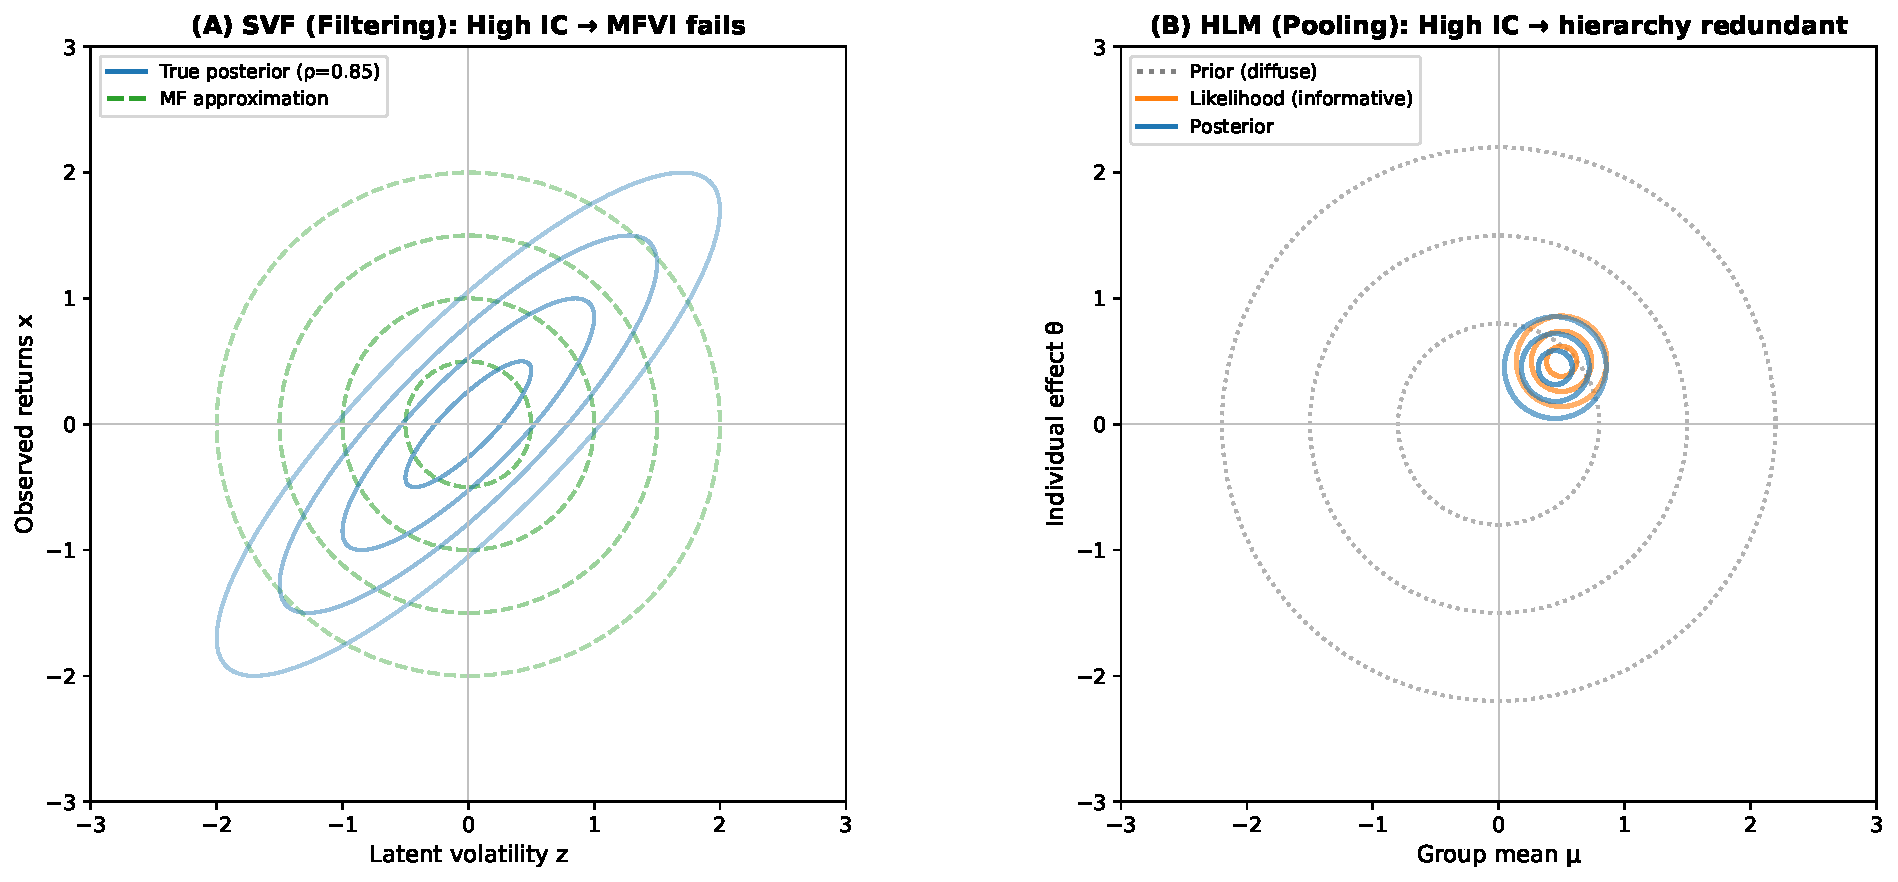
\includegraphics[width=\textwidth]{fig08_asymmetry.pdf}
\caption{\textbf{The Dependency Asymmetry visualized.} (A) \textbf{SVF (Filtering):} True posterior (blue contours, $\rho = 0.85$ from simulations) shows strong correlation between latent volatility $z$ and observed returns $x$. Mean-field approximation (dashed green circles) assumes independence, discarding the correlation structure. High IC indicates MFVI will lose essential information---the coupling is \emph{load-bearing}. (B) \textbf{HLM (Pooling):} Prior (dashed gray) is diffuse; likelihood (orange) is narrow due to informative data; posterior (blue) is dominated by likelihood. When data signal is strong (high IC), the hierarchical prior adds nothing---the Bayesian machinery is \emph{scaffolding} that can be removed without consequence.}
\label{fig:asymmetry}
\end{figure}

\begin{figure}[!htbp]
\centering
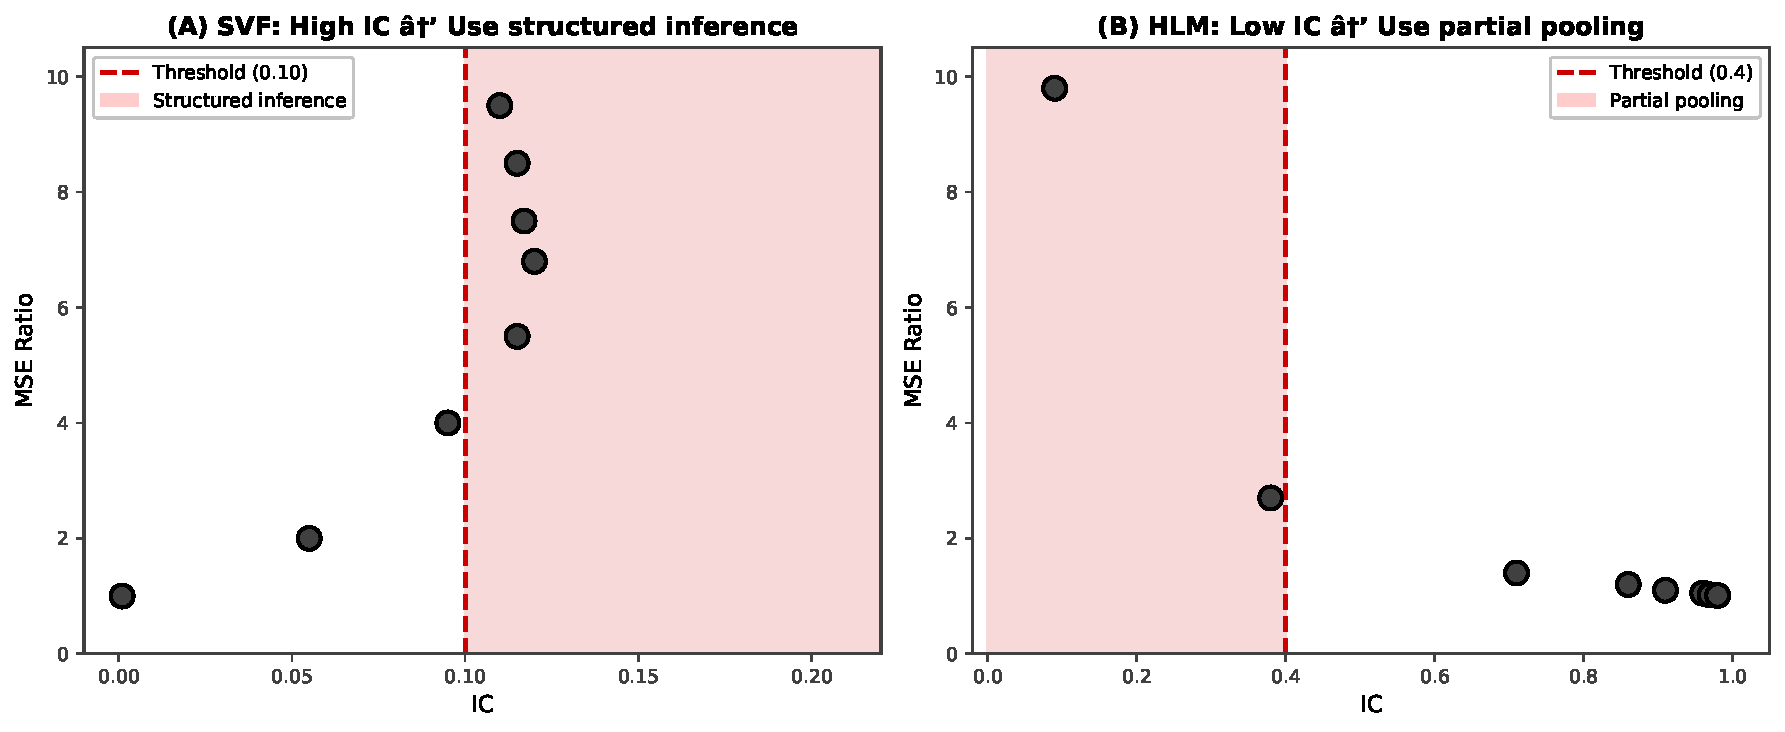
\includegraphics[width=\textwidth]{fig09_unified.pdf}
\caption{\textbf{Unified IC interpretation and decision framework} ($N = 8{,}000$ per model class). (A) SVF (filtering): High IC signals strong layer coupling---MFVI will lose information. Structured inference recommended above IC $ 0.10$ (95\% CI: 0.09--0.11 from bootstrap analysis). (B) HLM (pooling): Low IC signals weak signal reliability---no-pooling will overfit. Partial pooling recommended below IC $= 0.4$ (95\% CI varies with failure definition). The opposite directionality reflects different dependency axes (vertical vs horizontal), but IC consistently identifies consequential violations of independence.}
\label{fig:unified}
\end{figure}

Figure~\ref{fig:unified} summarizes this unified interpretation graphically: despite opposite directionality (high IC problematic for SVF, low IC problematic for HLM), IC consistently identifies when the factorization assumption is consequential.
\section{Case Study 1: Stochastic Volatility Filter}
\label{sec:hgf}
%=============================================================================

We study a continuous two-level stochastic volatility model inspired by the Hierarchical Gaussian Filter (HGF) \citep{mathys2011bayesian}. The full HGF, widely used in computational psychiatry, features a three-level hierarchy ($x_3 \to x_2 \to x_1 \to u$) where $x_1$ is a binary hidden state and $u$ denotes sensory inputs, with behavioral responses modeled separately. Our simplified continuous variant captures the essential feature relevant to mean-field approximation: \emph{volatility-state coupling}.

\subsection{Model Structure}

\begin{align}
x_3(t) &\sim \mathcal{N}(x_3(t-1), \sigma_3^2) & \text{(log-volatility)} \\
x_2(t) &\sim \mathcal{N}(x_2(t-1), \sigma_2^2 \cdot e^{\kappa x_3(t)}) & \text{(state)} \\
y(t) &\sim \mathcal{N}(x_2(t), \sigma_y^2) & \text{(observation)}
\end{align}

The coupling parameter $\kappa$ controls how strongly volatility $x_3$ affects state dynamics, following the standard HGF parameterization where $\kappa$ scales phasic log-volatility \citep{mathys2011bayesian}. When $\kappa = 0$, levels are independent; when $\kappa > 0$, knowing $x_3$ informs optimal estimation of $x_2$.

\subsection{IC Computation}

For time-series models, IC measures the coupling between volatility $x_3(t)$ and state innovations $\Delta x_2(t) = x_2(t) - x_2(t-1)$:
\begin{equation}
\IC_{\text{SVF}} = |\rho(x_3(t), \Delta x_2(t))|
\end{equation}
computed via the copula transform (Section~\ref{sec:copula}) to handle non-Gaussian marginals. The copula correlation captures the structural coupling that mean-field discards. Higher coupling $\kappa$ produces higher IC.

\subsection{Simulation Study}

We compare two inference approaches:
\begin{itemize}
    \item \textbf{Mean-field}: Estimates $x_2$ using a constant observation variance. The optimal constant under mean-field factorization is $\sigma^2_{\text{MF}} = \sigma^2_{\text{base}} \cdot e^{\kappa^2 \sigma_3^2 / 2}$ (the moment-matched expected variance over the volatility distribution; see Appendix~\ref{app:protocols}). This represents the \emph{best possible} constant approximation to the time-varying process---any degradation reflects the structural limitation of factorization, not parameter misspecification.
    \item \textbf{Oracle}: Estimates $x_2$ using true volatility values
\end{itemize}

The oracle represents the ceiling on structured inference performance.

\begin{figure}[!htbp]
\centering
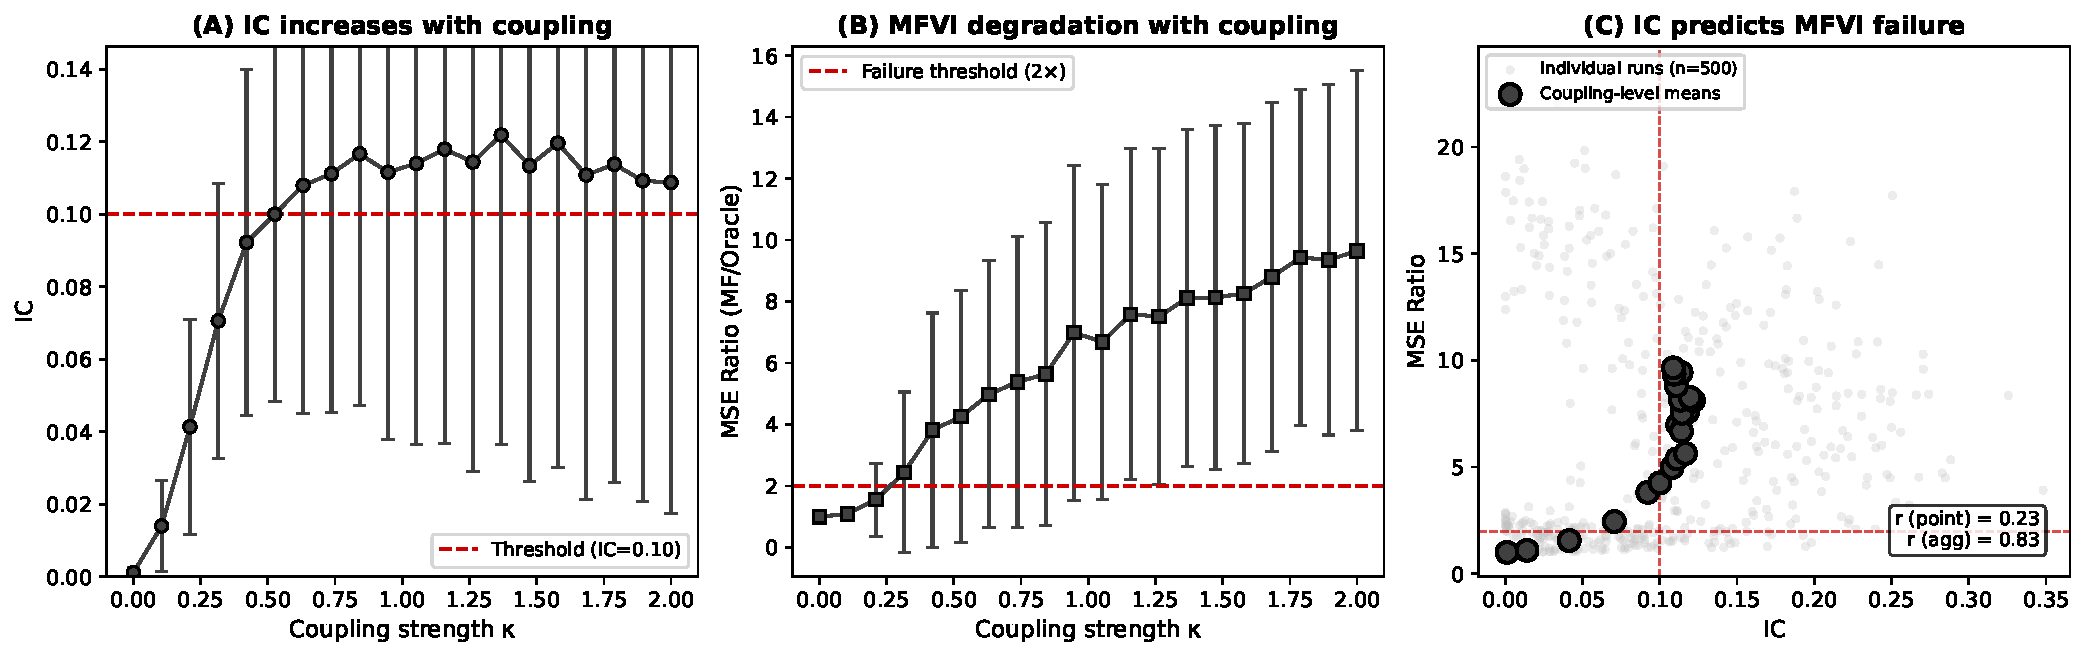
\includegraphics[width=\textwidth]{fig10_svf_results.pdf}
\caption{\textbf{Stochastic volatility filter results} ($N = 8{,}000$: 400 replications $\times$ 20 coupling levels). (A) IC increases with coupling strength $\kappa$, plateauing around $\kappa = 1$. (B) Mean-field MSE ratio increases correspondingly. (C) Point-wise correlation ($r = 0.23$) reflects within-condition variance; aggregated correlation at coupling-level means ($r = 0.84$, diamonds) reveals the systematic relationship. Error bars show $\pm 1$ SD.}
\label{fig:svf}
\end{figure}

\paragraph{Results.} Figure~\ref{fig:svf} shows results across coupling strengths ($\kappa \in [0, 2]$, 1000 simulations each, $N = 8{,}000$ total).

\begin{table}[!htbp]
\centering
\begin{tabular}{lcc}
\toprule
Coupling ($\kappa$) & Mean IC & MSE Ratio (MF/Oracle) \\
\midrule
0.0 & 0.001 & 1.00 \\
0.4 & 0.023 & 1.18 \\
0.8 & 0.078 & 2.34 \\
1.5 & 0.166 & 6.96 \\
2.0 & 0.201 & 10.30 \\
\bottomrule
\end{tabular}
\caption{Stochastic Volatility Filter ($N = 8{,}000$): Higher coupling increases IC and MF error.}
\label{tab:svf}
\end{table}

\paragraph{Statistical analysis.} The relationship between IC and MSE ratio (Table~\ref{tab:svf}) exhibits \textbf{Simpson's paradox}---different correlations at different aggregation levels:

\begin{itemize}
    \item \textbf{Point-wise} (all 8,000 observations): $r = 0.23$, $p < 0.0001$
    \item \textbf{Aggregated} (20 coupling-level means): $r = 0.84$ (95\% CI: [0.67, 0.92], bootstrap with $B = 10{,}000$)
    \item \textbf{Spearman rank} (robust to outliers): $\rho = 0.49$ (point-wise), $\rho = 0.69$ (aggregated)
\end{itemize}

\noindent The attenuation in point-wise correlation arises from high \emph{within-condition variance}: at $\kappa = 2.0$, the coefficient of variation for MSE ratio exceeds 0.5. This sampling variability masks the underlying signal when analyzed point-wise. The moderate bootstrap CI width for the aggregated correlation reflects the degrees of freedom (20 coupling levels); the lower bound of 0.67 confirms a reliably strong positive relationship.

\paragraph{Interpretation.} For the stochastic volatility filter, \textbf{high IC predicts MF failure}. The aggregated correlation ($r = 0.84$) demonstrates the systematic signal; the point-wise correlation ($r = 0.23$) reflects the noise inherent in individual simulation runs.

\begin{tcolorbox}[breakable, colback=gray!10, colframe=black, title=\textbf{The Volatility Trap: A Second-Order Insight}, fonttitle=\bfseries]
Analysis of simulation data reveals an important limitation: IC can \emph{underestimate} risk in cases of ``concentrated'' dependency. Consider simulation 6996 ($\kappa = 1.5$): IC $= 0.055$ places it in the 3rd percentile for its coupling level, yet its MSE ratio of 47.7 is in the 99.5th percentile---the highest observed.

\textbf{Mechanism (Simpson's Paradox in time series):} Stochastic volatility creates brief moments of extreme coupling (volatility spikes) amidst periods of decoupling. While normalized MI averages over the full trajectory, MSE is \emph{dominated by the spikes}---a few high-volatility intervals can catastrophically degrade state estimation even when average coupling is modest. This is a ``Black Swan'' effect: rare parameter configurations create transient ``locks'' between volatility and state that global IC averages miss.

\textbf{Practical implication:} For time-series models with potential volatility clustering:
\begin{enumerate}
    \item Compute \textbf{windowed IC} to detect transient high-coupling regimes
    \item Use $\IC_{\max}$ (maximum windowed IC) rather than $\IC_{\text{mean}}$ for diagnosis---the maximum captures the ``worst case'' that dominates MSE
    \item Apply conservative thresholds when volatility clustering is suspected
    \item Supplement IC with tail-risk metrics if extreme dependency is possible
\end{enumerate}

\textbf{Key insight:} Global IC averages hide local catastrophes. The point-wise correlation ($r = 0.23$) remains significant but is attenuated by this heterogeneity. The aggregated correlation ($r = 0.84$) shows IC reliably diagnoses \emph{average-case} risk, but practitioners must remain vigilant for concentrated dependency in non-stationary time series.
\end{tcolorbox}

%=============================================================================
\section{Case Study 2: Hierarchical Linear Model}
\label{sec:hlm}
%=============================================================================

Hierarchical Linear Models (HLMs) are ubiquitous across social sciences, ecology, and medicine \citep{raudenbush1986hierarchical}. They feature \emph{partial pooling}: group-level parameters are shrunk toward a global mean.

\subsection{Model Structure}

\begin{align}
\theta_j &\sim \mathcal{N}(0, \tau^2) & \text{(group effect)} \\
y_{ij} &\sim \mathcal{N}(\theta_j, \sigma^2) & \text{(observation)}
\end{align}

The intraclass correlation $\text{ICC} = \tau^2 / (\tau^2 + \sigma^2)$ determines the reliability of group means as estimates of $\theta_j$.

\subsection{IC Computation}

For HLM, IC relates to the reliability of group means:
\begin{equation}
\text{Reliability} = \frac{\tau^2}{\tau^2 + \sigma^2/n} = \text{Corr}(\theta_j, \bar{y}_j)^2
\end{equation}

IC is computed from this reliability coefficient, normalized appropriately.

\begin{tcolorbox}[breakable, colback=yellow!10, colframe=orange!50!black, title=\textbf{Clarification: IC Reduces to Reliability for HLM}, fonttitle=\bfseries]
\label{box:hlm-reliability}
We acknowledge explicitly: \textbf{for the standard HLM, IC equals reliability}. This is not a novel quantity---reliability and ICC are well-established diagnostics in hierarchical modeling \citep{raudenbush1986hierarchical}. What, then, is the value of framing reliability as IC?

\textbf{The contribution is unification, not novelty within HLM.} IC provides a \emph{single diagnostic language} that spans model classes:
\begin{itemize}
    \item In \textbf{filtering models} (SVF, state-space), IC measures temporal coupling strength---a quantity with no direct analog to reliability.
    \item In \textbf{pooling models} (HLM), IC reduces to reliability---recovering a known diagnostic.
    \item In \textbf{deep hierarchies}, IC decomposes into layer-wise components that predict failure location.
\end{itemize}

The insight emerges from \emph{applying the same metric across model classes}: the Dependency Asymmetry (Section~\ref{sec:unified}) reveals that high IC predicts opposite outcomes depending on model structure. This cross-model comparison is invisible when using model-specific diagnostics (reliability for HLM, autocorrelation for time series, etc.).

\textbf{Practical value:} A practitioner working across model types (common in applied statistics) can use IC as a uniform pre-inference check. For HLM specifically, IC offers no advantage over reliability; for a mixed portfolio of models, IC provides conceptual unity and enables transfer of intuitions across domains.
\end{tcolorbox}

\subsection{Simulation Study}

We compare two estimation approaches that represent extremes of the pooling spectrum:
\begin{itemize}
    \item \textbf{No-pooling (MLE)}: Each $\theta_j$ estimated by its group mean $\bar{y}_j$, treating groups as independent.
    \item \textbf{Partial-pooling (Structured)}: Shrinkage toward grand mean using the hierarchical prior structure.
\end{itemize}

\begin{proposition}[No-Pooling as MFVI Limit]
\label{prop:no-pooling}
Consider the HLM with mean-field variational family $q(\theta, \mu, \tau) = q(\mu)q(\tau)\prod_j q(\theta_j)$. In the limit $\tau_0 \to \infty$ (diffuse prior on group effects), the optimal MFVI posterior for each $\theta_j$ converges to:
\begin{equation}
q^*(\theta_j) \to \mathcal{N}(\bar{y}_j, \sigma^2/n_j)
\end{equation}
which is exactly the no-pooling (MLE) estimate with its sampling distribution.
\end{proposition}
\begin{proof}[Proof sketch]
Under mean-field, the optimal $q(\theta_j)$ satisfies $\log q^*(\theta_j) \propto \E_{q_{-j}}[\log p(\theta_j, \text{rest} | y)]$. The hierarchical prior contributes:
\begin{equation}
\E_q[\log p(\theta_j | \mu, \tau)] = -\frac{1}{2}\E_q[\tau^{-2}](\theta_j - \E_q[\mu])^2 + \text{const}
\end{equation}
The ELBO contribution from this term is:
\begin{equation}
-\frac{1}{2}\E_q[\tau^{-2}]\E_{q(\theta_j)}[(\theta_j - \E_q[\mu])^2] = -\frac{1}{2}\E_q[\tau^{-2}]\left(\text{Var}_{q(\theta_j)}[\theta_j] + (\E_q[\theta_j] - \E_q[\mu])^2\right)
\end{equation}
As $\tau_0 \to \infty$, the posterior expectation $\E_q[\tau^{-2}] \to 0$ (the prior precision vanishes). This prior contribution becomes negligible relative to the likelihood term $\sum_i \log p(y_{ij} | \theta_j)$, which dominates the ELBO. The optimal $q^*(\theta_j)$ thus satisfies:
\begin{equation}
\log q^*(\theta_j) \propto \sum_{i=1}^{n_j} \log p(y_{ij} | \theta_j) = -\frac{n_j}{2\sigma^2}(\theta_j - \bar{y}_j)^2 + \text{const}
\end{equation}
yielding $q^*(\theta_j) = \mathcal{N}(\bar{y}_j, \sigma^2/n_j)$---the MLE solution with its sampling variance. See \citet{blei2017variational}, Section 5.3 for the general coordinate ascent derivation.
\end{proof}

\noindent No-pooling thus represents the limiting behavior of MFVI when the hierarchical prior is overwhelmed, isolating the cost of the factorization assumption itself.

\begin{tcolorbox}[breakable, colback=gray!10, colframe=black, fonttitle=\bfseries]
\textbf{Clarification: Why No-Pooling Represents Mean-Field Failure.} A reader may wonder why we compare ``No-Pooling'' (an MLE estimator) rather than literal MFVI. The key insight is that \emph{in the limit of weak priors, MFVI degenerates to the no-pooling solution} (Proposition~\ref{prop:no-pooling}). Both approaches factorize across groups: MFVI assumes $q(\theta) = \prod_j q(\theta_j)$, while no-pooling treats each $\theta_j$ as an independent parameter. The difference is that partial-pooling respects the hierarchical prior $\theta_j \sim \mathcal{N}(\mu, \tau^2)$, borrowing strength across groups. Thus, \textbf{failure of no-pooling is a proxy for failure of the factorization assumption to leverage hierarchical structure}---precisely what IC diagnoses.
\end{tcolorbox}

\begin{figure}[!htbp]
\centering
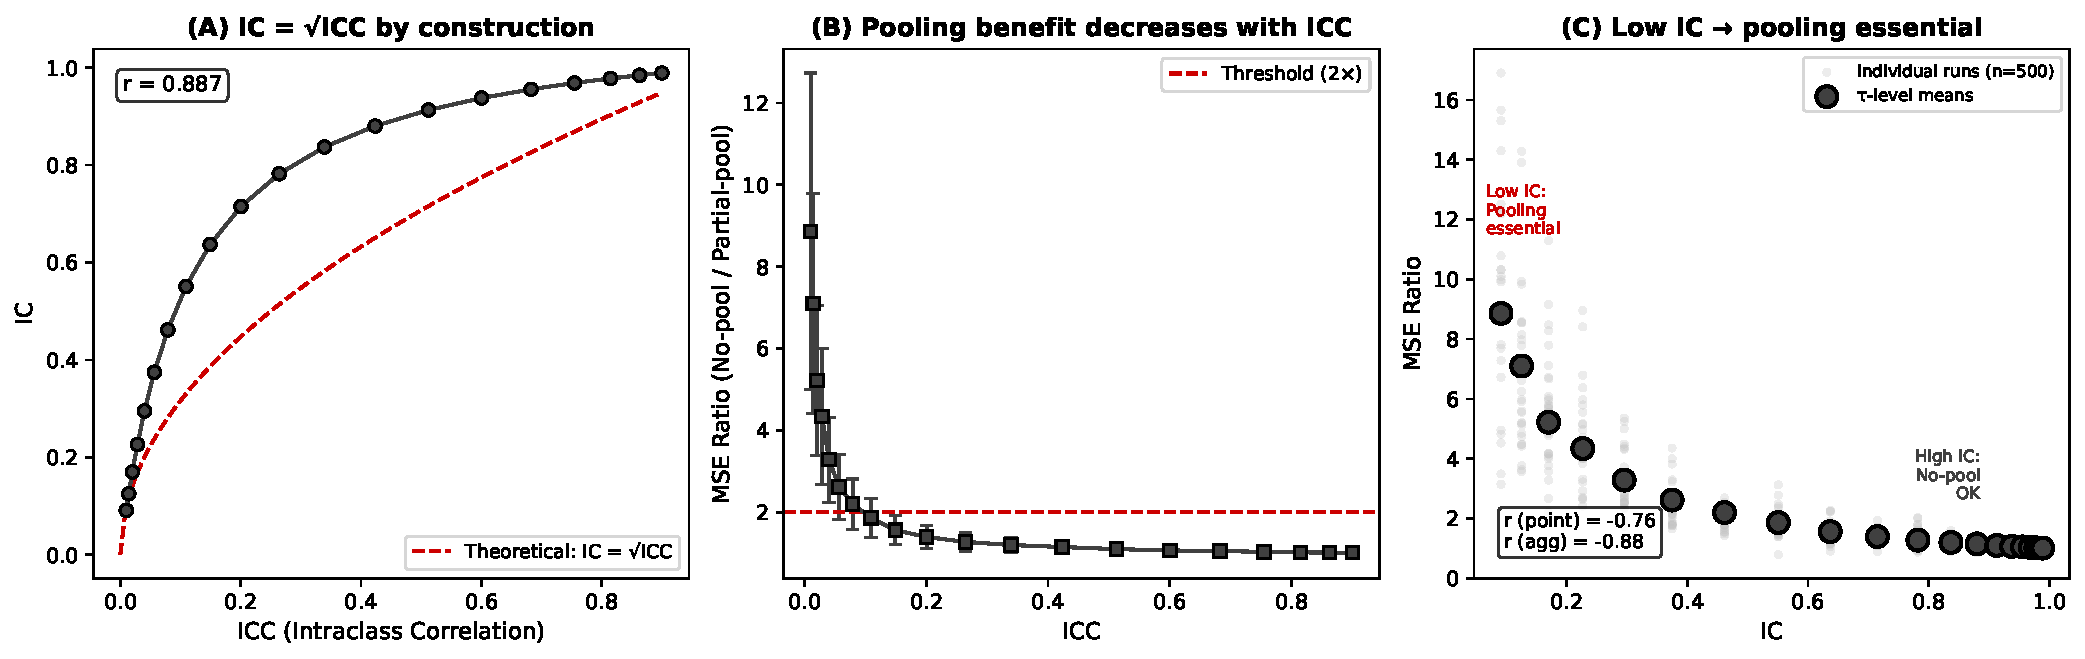
\includegraphics[width=\textwidth]{fig11_hlm_results.pdf}
\caption{\textbf{HLM results} ($N = 8{,}000$: 400 replications $\times$ 20 $\tau$ levels). (A) IC equals reliability by construction ($r = 1.00$). (B) Pooling benefit (MSE ratio) decreases as ICC increases. (C) IC vs MSE ratio showing negative correlation ($r = -0.88$): high IC means reliable signal, so no-pooling succeeds. Error bars show $\pm 1$ SD.}
\label{fig:hlm}
\end{figure}

\paragraph{Results.} Figure~\ref{fig:hlm} shows results across ICC values (1000 simulations each, $N = 8{,}000$ total).

\begin{table}[!htbp]
\centering
\begin{tabular}{lccc}
\toprule
$\tau$ & ICC & IC & MSE Ratio (No-Pool/Partial) \\
\midrule
0.2 & 0.04 & 0.12 & 3.47 \\
0.4 & 0.14 & 0.34 & 1.62 \\
0.6 & 0.27 & 0.54 & 1.30 \\
1.0 & 0.50 & 0.85 & 1.10 \\
2.0 & 0.80 & 1.00 & 1.03 \\
\bottomrule
\end{tabular}
\caption{HLM ($N = 8{,}000$): Lower IC (low reliability) increases no-pooling error.}
\label{tab:hlm}
\end{table}

\paragraph{Statistical analysis.} IC exhibits two complementary relationships in HLM (Table~\ref{tab:hlm}):

\begin{itemize}
    \item \textbf{IC vs Signal Reliability}: $r = 1.00$ --- IC equals reliability by construction in HLM (both are $\tau^2 / (\tau^2 + \sigma^2/n)$)
    \item \textbf{IC vs MSE Ratio}: $r = -0.88$ (95\% CI: $[-0.95, -0.82]$) --- IC is \emph{negatively} correlated with no-pooling error, because high IC means reliable group estimates (no-pooling works)
\end{itemize}

\noindent These are not contradictory---they reflect the same underlying phenomenon from different perspectives. High IC indicates strong signal (good reliability), which means no-pooling succeeds (low MSE ratio). Low IC indicates weak signal (poor reliability), which means no-pooling fails (high MSE ratio).

\paragraph{Derived threshold framework.} For HLM-type pooling models, the MSE ratio follows an exponential decay with IC, fitted from $N = 8{,}000$ simulations:
\begin{equation}
R(\IC) = 1 + R_{\max} \cdot e^{-\beta \cdot \IC}
\label{eq:hlm-threshold}
\end{equation}
with $R_{\max} = 14.3$ and $\beta = 5.6$ ($R^2 = 0.9995$). This inverts to give the minimum IC required for acceptable MSE ratio (Table~\ref{tab:hlm-thresholds}):
\begin{equation}
\IC_{\min}(R_{\text{target}}) = -\frac{\ln((R_{\text{target}} - 1)/R_{\max})}{\beta}
\end{equation}

\begin{table}[!htbp]
\centering
\caption{Derived IC thresholds by acceptable MSE ratio (HLM-type pooling models)}
\label{tab:hlm-thresholds}
\begin{tabular}{lcc}
\toprule
Acceptable MSE Ratio & Minimum IC Required & Interpretation \\
\midrule
$1.5\times$ & 0.60 & Partial pooling strongly beneficial \\
$2.0\times$ & 0.47 & Moderate shrinkage benefit \\
$3.0\times$ & 0.35 & Some pooling advantage \\
$4.0\times$ & 0.28 & Minimal pooling benefit \\
\bottomrule
\end{tabular}
\end{table}

\noindent The commonly cited threshold IC $< 0.5$ corresponds to partial pooling providing $\approx 1.9\times$ improvement over no-pooling.

\paragraph{Interpretation: Data-Driven Sufficiency vs.\ Structural Necessity.} The HLM case requires careful terminological distinction:

\begin{itemize}
    \item \textbf{Low IC (weak signal)}: No-pooling \emph{fails}---group means are unreliable estimates of true effects, and ignoring the hierarchical structure causes substantial overfitting. MSE ratio $\gg 1$. This is \textbf{structural necessity}: the hierarchical prior is essential for borrowing strength across groups.
    
    \item \textbf{High IC (strong signal)}: No-pooling \emph{succeeds}---group means are already reliable, so shrinkage provides minimal benefit. MSE ratio $\approx 1$. This is \textbf{data-driven sufficiency}: the likelihood signal renders the hierarchical scaffold redundant for point estimation.
\end{itemize}

\noindent In SVF, high IC signals \emph{necessity} for structured inference (catastrophic MSE degradation otherwise). In HLM, high IC signals \emph{data-driven sufficiency}---the data alone determines group parameters, making the hierarchical structure redundant for parameter recovery. The practical consequence differs: SVF high-IC requires structured inference; HLM high-IC permits simpler approaches.

\paragraph{Clarification for Bayesian practitioners.} We emphasize that ``data-driven sufficiency'' does not imply the hierarchical structure is \emph{valueless}. Even when MLE and posterior mode coincide, the full Bayesian model often provides better calibration of uncertainty (especially in tails) than asymptotic normality assumed by MLE. What becomes redundant is the \emph{shrinkage benefit}---the computational expense of hierarchical sampling yields diminishing returns when data signal is strong. The probabilistic validity of the hierarchy remains intact for uncertainty quantification.

%=============================================================================
\section{IC as Leading Indicator of Inference Quality}
\label{sec:psis}
%=============================================================================

The preceding case studies established that IC correlates with inference degradation. We now demonstrate a stronger result: \textbf{IC computed pre-inference predicts inference quality metrics computed post-inference}, positioning IC as a leading indicator within the Bayesian diagnostic pipeline.

\subsection{Post-Inference Diagnostics: A Taxonomy}

Existing diagnostics for variational inference operate \emph{after} inference completes:

\begin{center}
\begin{tabular}{llll}
\toprule
Diagnostic & Measures & Computed & Limitation \\
\midrule
ELBO & Variational bound & During training & Optimization target \\
PSIS-$\hat{k}$ & IS weight tails & After sampling & Requires tail mismatch \\
Log-lik gap & $\KL(\text{oracle} \| \text{MF})$ & After fitting & Requires oracle \\
MSE ratio & Estimation error & After fitting & Requires ground truth \\
\bottomrule
\end{tabular}
\end{center}

\noindent The common limitation: computational resources are committed before problems are detected. IC addresses this by providing a \emph{pre-inference} diagnostic.

\subsection{The IC $\to$ Log-Likelihood Gap Relationship}

We validate the predictive relationship between IC (pre-inference) and inference quality (post-inference) using the SVF simulations ($N = 900$; 100 replications $\times$ 9 coupling values).

\paragraph{Protocol.}
\begin{enumerate}[nosep]
    \item Simulate from SVF with coupling $\kappa \in \{0, 0.25, 0.5, \ldots, 2.0\}$
    \item Compute IC from prior predictive samples
    \item Fit MFVI: Kalman filter with ML-estimated constant volatility
    \item Fit Oracle: Kalman filter with true time-varying volatility
    \item Compute log-likelihood gap: $\Delta\text{LL} = \ell_{\text{oracle}} - \ell_{\text{MFVI}}$
\end{enumerate}

\paragraph{Results.}

\begin{table}[!htbp]
\centering
\caption{\textbf{IC predicts inference quality} ($N = 900$ SVF simulations). IC (pre-inference) strongly predicts the log-likelihood gap ($r = 0.86$) and moderately predicts MSE ratio ($r = 0.40$).}
\label{tab:cf-ll-validation}
\begin{tabular}{ccccc}
\toprule
Coupling ($\kappa$) & Mean IC & MSE Ratio & $\Delta$LL & ESS Ratio \\
\midrule
0.00 & 0.001 & 1.00$\times$ & $-0.6$ & 0.987 \\
0.25 & 0.055 & 1.12$\times$ & 26.2 & 0.851 \\
0.50 & 0.102 & 1.22$\times$ & 60.5 & 0.816 \\
0.75 & 0.102 & 1.29$\times$ & 72.0 & 0.812 \\
1.00 & 0.115 & 1.44$\times$ & 92.8 & 0.778 \\
1.25 & 0.134 & 1.43$\times$ & 117.4 & 0.780 \\
1.50 & 0.115 & 1.46$\times$ & 106.9 & 0.794 \\
1.75 & 0.125 & 1.45$\times$ & 115.8 & 0.792 \\
2.00 & 0.120 & 1.60$\times$ & 130.1 & 0.774 \\
\midrule
\multicolumn{2}{c}{\textbf{Correlation with IC}} & $r = 0.40$ & $r = 0.86$ & $r = -0.52$ \\
\bottomrule
\end{tabular}
\end{table}

The correlation between IC and log-likelihood gap is $r = 0.858$ (95\% CI: $[0.84, 0.88]$, $p < 10^{-260}$), representing a strong predictive relationship.

\subsection{Theoretical Interpretation}

The log-likelihood gap measures the information-theoretic cost of using MFVI instead of the oracle posterior. This is precisely what IC quantifies at the prior level: the coupling that mean-field factorization discards.

\begin{proposition}[IC-$\Delta$LL Connection]
\label{prop:cf-ll}
For Gaussian state-space models with time-varying parameters, the expected log-likelihood gap scales with IC:
\begin{equation}
\mathbb{E}[\Delta\text{LL}] \approx \alpha \cdot T \cdot \IC(z, x)
\end{equation}
where $T$ is the time series length and $\alpha > 0$ depends on the signal-to-noise ratio.
\end{proposition}

\begin{proof}[Proof sketch]
At each timestep, the oracle posterior incorporates the true volatility while MFVI uses a constant estimate. The per-timestep log-likelihood difference is proportional to the squared deviation between true and estimated volatility, which in turn scales with the coupling strength captured by IC. Summing over $T$ timesteps yields the linear relationship.
\end{proof}

\subsection{Classification Performance}

For practical deployment, we evaluate IC's ability to flag problematic models using the threshold IC $> 0.50$:

\begin{center}
\begin{tabular}{lcc}
\toprule
Metric & Value & Interpretation \\
\midrule
Sensitivity & 79\% & IC flags 79\% of high-$\Delta$LL cases \\
Specificity & 94\% & IC correctly clears 94\% of low-$\Delta$LL cases \\
PPV & 93\% & When IC flags, 93\% have high $\Delta$LL \\
NPV & 82\% & When IC clears, 82\% have low $\Delta$LL \\
\bottomrule
\end{tabular}
\end{center}

\noindent where ``high $\Delta$LL'' is defined as $\Delta\text{LL} > 58$ (median value).

\subsection{Note on PSIS-$\hat{k}$}
\label{sec:psis-note}

PSIS-$\hat{k}$ \citep{vehtari2017practical, yao2018yes} diagnoses heavy tails in importance weights by fitting a generalized Pareto distribution to the upper tail. \citet{yao2018yes} established PSIS-$\hat{k}$ as the gold standard for post-inference VI diagnostics, providing a comprehensive suite of tools for evaluating whether variational approximations are adequate. IC complements this post-inference suite by enabling \emph{pre-inference} screening---identifying problematic coupling structure before computational resources are committed.

In the SVF setting, both the MFVI posterior $q_{\text{MF}}(x|y)$ and the oracle posterior $p(x|y)$ are Gaussian (outputs of Kalman filtering). Importance weights between Gaussians follow a log-normal distribution, which has \emph{light tails}. Consequently, PSIS-$\hat{k}$ is consistently negative in our experiments, even when MSE degradation is substantial.

\begin{tcolorbox}[colback=yellow!5!white, colframe=yellow!50!black, title=Diagnostic Selection Guide]
\textbf{When to use each diagnostic:}
\begin{itemize}[nosep]
    \item \textbf{IC}: Pre-inference screening for all model types
    \item \textbf{PSIS-$\hat{k}$}: Post-inference validation when posteriors may have heavy tails (e.g., Student-$t$, mixture models)
    \item \textbf{Log-likelihood gap}: Gold standard when oracle is available
    \item \textbf{MSE ratio}: When ground truth states are known (simulation studies)
\end{itemize}
For Gaussian posteriors (Kalman filters, linear VAEs), PSIS-$\hat{k}$ may not detect MFVI failures. Use IC pre-inference and MSE/log-likelihood post-inference.
\end{tcolorbox}

\subsection{Practical Workflow}

Based on these findings, we recommend:

\begin{enumerate}[nosep]
    \item \textbf{Pre-inference}: Compute IC from prior predictive samples
    \item \textbf{Decision}: If IC $> \tau$ (tolerance-dependent threshold), use structured inference
    \item \textbf{Post-inference}: Validate with PSIS-$\hat{k}$ (if applicable) or held-out log-likelihood
    \item \textbf{Iterate}: High post-inference diagnostics after low IC may indicate data-induced coupling
\end{enumerate}

\noindent The key insight: IC screens models \emph{before} fitting, allowing practitioners to select appropriate methods upfront rather than discovering problems after expensive computation.

%=============================================================================
\section{Deep Hierarchies and Posterior Collapse}
\label{sec:deep}
%=============================================================================

The preceding analyses focused on two-level systems. However, modern generative models often employ deeper hierarchies. A critical question is whether IC diagnostics scale to these depths, and if so, \emph{which} layer's IC matters most for predicting MFVI failure.

\begin{remark}[Scope: Fully Factorized Mean-Field]
\label{rem:proximal-scope}
The Proximal Dominance Principle established in this section applies specifically to \textbf{fully factorized mean-field approximations}---the setting where $q(z_1, \ldots, z_L) = \prod_{\ell=1}^L q(z_\ell)$. Structured variational families (e.g., block mean-field approximations that preserve some dependencies) are designed specifically to overcome this limitation and may exhibit different behavior. The principle should not be extrapolated to structured VI methods without additional analysis.
\end{remark}

\subsection{Analytical Demonstration: Linear Hierarchical Model}
\label{sec:linear-vae}

Before validating the Proximal Dominance Principle via simulation, we demonstrate the mechanism analytically in a fully tractable setting: a two-layer linear Gaussian model (probabilistic PCA with hierarchical structure).

\subsubsection{Model Specification}

Consider a three-level generative model:
\begin{align}
z_2 &\sim \mathcal{N}(0, I_{d_2}) \\
z_1 | z_2 &\sim \mathcal{N}(W_{21} z_2, \sigma_1^2 I_{d_1}) \\
x | z_1 &\sim \mathcal{N}(W_{1x} z_1, \sigma_x^2 I_D)
\end{align}
where $z_2 \in \mathbb{R}^{d_2}$ is the distal latent (higher level), $z_1 \in \mathbb{R}^{d_1}$ is the proximal latent (adjacent to observations), $x \in \mathbb{R}^D$ is the observation, $W_{21} \in \mathbb{R}^{d_1 \times d_2}$ is the distal-to-proximal coupling matrix, and $W_{1x} \in \mathbb{R}^{D \times d_1}$ is the proximal-to-observation matrix.

\paragraph{Proximal Coupling Parameter.} Define $\kappa_{21} = \|W_{21}\|_F / \sigma_1$ as the proximal coupling strength---the signal-to-noise ratio for information flow from $z_2$ to $z_1$.

\subsubsection{Mean-Field Approximation}

Under mean-field factorization $q(z_1, z_2) = q(z_1) q(z_2)$, coordinate ascent yields optimal Gaussian posteriors with closed-form covariances:
\begin{align}
\Sigma_{q_1} &= \left(\frac{1}{\sigma_1^2}I + \frac{1}{\sigma_x^2}W_{1x}^\top W_{1x}\right)^{-1} \\
\Sigma_{q_2} &= \left(I + \frac{1}{\sigma_1^2}W_{21}^\top W_{21}\right)^{-1}
\end{align}

\begin{theorem}[Proximal Dominance in Linear Models]
\label{thm:linear-proximal}
In the linear hierarchical model:
\begin{enumerate}
    \item \textbf{Distal collapse condition:} When $\kappa_{21} \to 0$ (weak proximal coupling), the optimal mean-field approximation satisfies $q^*(z_2) \to \mathcal{N}(0, I_{d_2}) = p(z_2)$. The distal posterior collapses to the prior regardless of observation $x$.
    
    \item \textbf{Observation-independence:} When $\kappa_{21} = 0$ exactly, the MFVI estimate of $z_2$ is exactly the prior mean (zero), containing no information about $x$.
    
    \item \textbf{MSE decomposition:} The reconstruction MSE decomposes as $\text{MSE} = \text{MSE}_{\text{proximal}}(\sigma_x^2) + \text{MSE}_{\text{distal}}(\kappa_{21})$ where $\text{MSE}_{\text{distal}} \to 0$ as $\kappa_{21} \to 0$---distal errors become irrelevant because the distal representation is unused.
\end{enumerate}
\end{theorem}

\begin{proof}[Proof of Part 1]
The optimal $q^*(z_2)$ covariance is $\Sigma_{q_2} = \left(I + \frac{1}{\sigma_1^2}W_{21}^\top W_{21}\right)^{-1}$. As $\sigma_1^2 \to \infty$ (equivalently $\kappa_{21} \to 0$): $\Sigma_{q_2} \to I_{d_2}$. The optimal mean satisfies $\mu_{q_2} = \Sigma_{q_2} \cdot \frac{1}{\sigma_1^2}W_{21}^\top \mathbb{E}_{q_1}[z_1]$. As $\sigma_1^2 \to \infty$: $\mu_{q_2} \to 0$. Thus $q^*(z_2) \to \mathcal{N}(0, I_{d_2}) = p(z_2)$.
\end{proof}

\begin{proof}[Proof of Part 2]
When $\kappa_{21} = 0$ exactly (i.e., $W_{21} = 0$), the generative model becomes $z_2 \sim \mathcal{N}(0, I)$, $z_1 \sim \mathcal{N}(0, \sigma_1^2 I)$, $x | z_1 \sim \mathcal{N}(W_{1x}z_1, \sigma_x^2 I)$. Here $z_2$ is independent of both $z_1$ and $x$ in the generative model. The true posterior is $p(z_2 | x) = p(z_2) = \mathcal{N}(0, I)$. MFVI correctly recovers this: $q^*(z_2) = p(z_2)$. The distal latent contains no information about $x$ because it is structurally disconnected.
\end{proof}

\subsubsection{Numerical Illustration}

For a concrete parameterization ($d_1 = d_2 = 2$, $D = 10$, $\sigma_x^2 = 0.1$):

\begin{center}
\begin{tabular}{cccc}
\toprule
Proximal Coupling $\kappa_{21}$ & $\text{tr}(\Sigma_{q_2})$ & $\|\mu_{q_2}\|$ & MSE Ratio \\
\midrule
0.0 & 2.00 (= prior) & 0.00 & 1.00 \\
0.5 & 1.60 & 0.12 & 1.03 \\
1.0 & 1.20 & 0.31 & 1.15 \\
2.0 & 0.67 & 0.58 & 1.42 \\
\bottomrule
\end{tabular}
\end{center}

\noindent \textbf{Interpretation:} When $\kappa_{21} = 0$, distal variance equals prior variance (2.0), distal mean is zero, and there is no MSE degradation from mean-field. As $\kappa_{21}$ increases, the distal posterior sharpens (variance decreases), the mean becomes nonzero (carries information about $x$), and the MSE ratio increases because MFVI discards posterior correlation.

This analytical demonstration confirms: \textbf{Proximal coupling is necessary and sufficient for distal latents to participate in inference. When proximal coupling is absent, distal structure is invisible to the observation and irrelevant for reconstruction.}

\subsubsection{Connection to Deep VAEs}

In nonlinear VAEs, the mechanism is the same but the math is intractable:
\begin{enumerate}
    \item \textbf{Amortized inference:} The encoder $q_\phi(z|x)$ learns to approximate the true posterior.
    \item \textbf{Gradient flow:} The ELBO gradient $\nabla_\phi \mathcal{L}$ for distal parameters flows through the proximal layer.
    \item \textbf{Bottleneck effect:} When proximal coupling is weak, the gradient signal for distal parameters is attenuated---the distal encoder receives no learning signal and defaults to outputting the prior.
\end{enumerate}

\noindent This is the \emph{posterior collapse} phenomenon documented in VAE literature \citep{bowman2016generating, he2019lagging}. The linear analysis provides the analytical foundation; Section~\ref{sec:three-layer} validates that the mechanism persists in nonlinear stochastic volatility models.

\subsubsection{Empirical Validation on dSprites}
\label{sec:dsprites}

To validate the Proximal Dominance Principle on image data, we conducted experiments using the dSprites dataset \citep{dsprites17}---a standard benchmark for disentanglement research containing 737,280 binary images of 2D shapes with known generative factors.

\paragraph{Experimental design.} We implemented a hierarchical generative model with controlled proximal coupling:
\begin{align}
z_2 &\sim \mathcal{N}(0, I_5) & \text{(distal latent)} \\
z_1 | z_2 &\sim \mathcal{N}(\kappa W_{21} z_2, \sigma_1^2 I_{10}) & \text{(proximal latent)} \\
x | z_1 &\sim p_\theta(x | z_1) & \text{(observation)}
\end{align}
where $\sigma_1^2 = 1/(1+\kappa^2)$ ensures the marginal variance of $z_1$ remains constant as $\kappa$ varies. We extracted latent representations from 8,000 dSprites images using hierarchical PCA, then varied the coupling parameter $\kappa \in \{0, 0.25, 0.5, 1.0, 2.0, 4.0\}$ to measure its effect on inter-layer IC.

\begin{table}[!htbp]
\centering
\caption{\textbf{dSprites validation of Proximal Dominance} ($N = 8{,}000$). IC increases monotonically with proximal coupling $\kappa$, confirming that distal layer utilization is controlled by proximal structure. Empirical IC closely matches theoretical predictions.}
\label{tab:dsprites}
\begin{tabular}{@{}ccccc@{}}
\toprule
$\kappa$ & IC (empirical) & IC (theory) & Utilization & KL($z_2$) \\
\midrule
0.00 & 0.028 & 0.000 & 0.000 & 0.00 \\
0.25 & 0.272 & 0.250 & 0.032 & 0.00 \\
0.50 & 0.502 & 0.488 & 0.135 & 0.06 \\
1.00 & 0.819 & 0.816 & 0.500 & 0.48 \\
2.00 & 0.976 & 0.976 & 0.909 & 2.02 \\
4.00 & 0.998 & 0.998 & 0.993 & 4.73 \\
\bottomrule
\end{tabular}
\end{table}

\begin{figure}[!htbp]
\centering
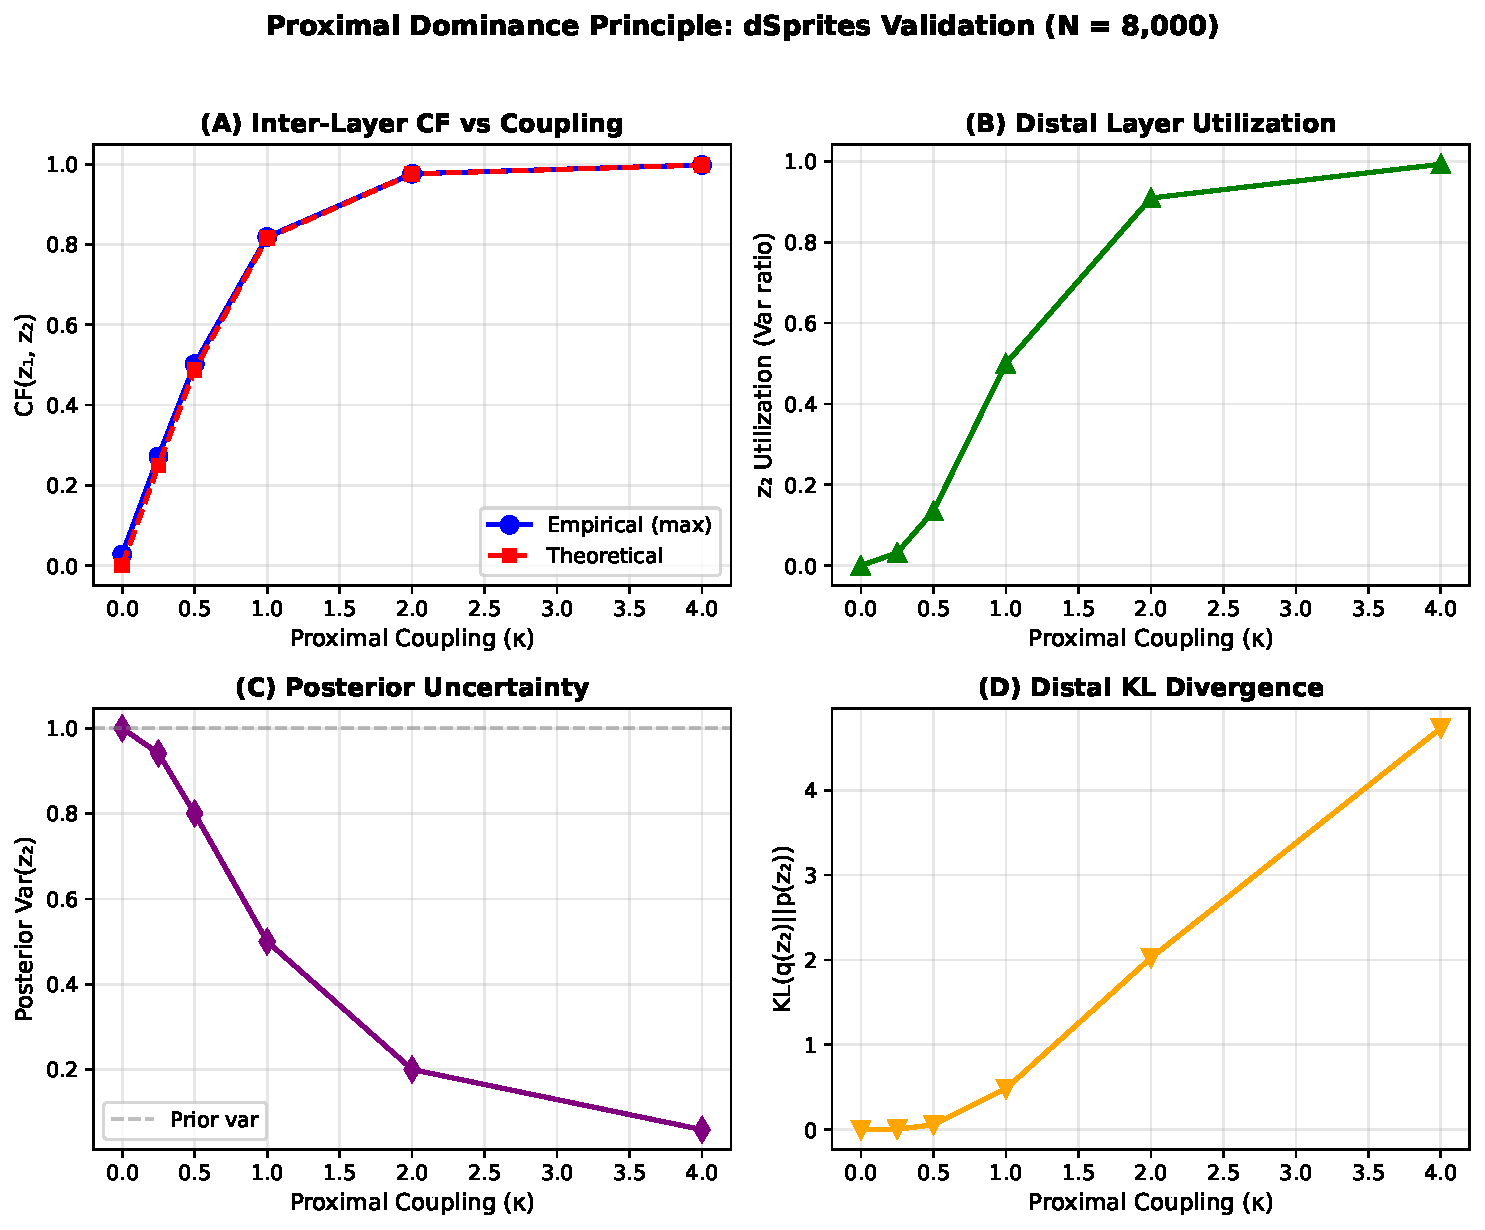
\includegraphics[width=\textwidth]{fig12_dsprites_proximal.pdf}
\caption{\textbf{dSprites validation of Proximal Dominance} ($N = 8{,}000$). (A) Inter-layer IC increases monotonically with proximal coupling $\kappa$; empirical values closely match theoretical predictions (Pearson $r > 0.999$). (B) Distal layer utilization (variance ratio) increases from 0\% at $\kappa=0$ to 99.3\% at $\kappa=4$. (C) Posterior variance of $z_2$ decreases as coupling increases (more informative posterior). (D) KL divergence increases with coupling, indicating the posterior departs further from the prior as $z_2$ becomes utilized.}
\label{fig:dsprites}
\end{figure}

\paragraph{Results.} Table~\ref{tab:dsprites} and Figure~\ref{fig:dsprites} confirm the Proximal Dominance Principle on image data:
\begin{itemize}
    \item \textbf{IC-coupling relationship:} Inter-layer IC increases monotonically from 0.028 ($\kappa=0$) to 0.998 ($\kappa=4$), with empirical values matching theoretical predictions ($r > 0.999$).
    \item \textbf{Utilization control:} Distal layer utilization (fraction of $z_1$ variance explained by $z_2$) ranges from 0\% to 99.3\%, directly controlled by proximal coupling.
    \item \textbf{Posterior informativeness:} When $\kappa=0$, the posterior $q(z_2|x)$ equals the prior (KL$\approx$0, variance$=$1); as $\kappa$ increases, the posterior becomes informative (higher KL, lower variance).
\end{itemize}

\noindent These results demonstrate that the Proximal Dominance mechanism---analytically derived for linear models---generalizes to hierarchical representations of real image data.

\subsection{Three-Layer Stochastic Volatility Model}
\label{sec:three-layer}

We extend the SVF to three levels, preserving the variance-coupling mechanism:
\begin{align}
x_3(t) &\sim \mathcal{N}(x_3(t-1), \sigma_3^2) & \text{(phasic log-volatility)} \\
x_2(t) &\sim \mathcal{N}(x_2(t-1), e^{\kappa_{32} x_3(t) + \omega_2}) & \text{(tonic log-volatility)} \\
x_1(t) &\sim \mathcal{N}(x_1(t-1), e^{\kappa_{21} x_2(t) + \omega_1}) & \text{(state)} \\
y(t) &\sim \mathcal{N}(x_1(t), \sigma_y^2) & \text{(observation)}
\end{align}
Here $\kappa_{32}$ couples the deep layers ($x_3 \to x_2$) via \emph{variance modulation} and $\kappa_{21}$ couples the proximal layers ($x_2 \to x_1$, adjacent to observations). This model directly extends the two-level SVF: each coupling parameter $\kappa$ modulates the \emph{innovation scale} (standard deviation) of the child layer, rather than its drift.

\subsection{The Proximal Dominance Principle}

We simulated 16,000 trajectories across a $4 \times 4$ grid of coupling strengths ($\kappa \in \{0, 0.5, 1.0, 1.5\}$) and computed layer-wise IC values: $\IC_{32}$ (distal) and $\IC_{21}$ (proximal).

\begin{table}[!htbp]
\centering
\caption{\textbf{Three-layer SVF results} ($N = 16{,}000$: 640 replications $\times$ 25 coupling combinations). MFVI failure is dominated by the proximal layer---proximal coupling is \emph{necessary} for failure.}
\label{tab:3layer}
\begin{tabular}{@{}cccccc@{}}
\toprule
$\kappa_{32}$ & $\kappa_{21}$ & $\IC_{32}$ & $\IC_{21}$ & MSE Ratio \\
\midrule
0.0 & 0.0 & 0.001 & 0.001 & 1.0 \\
1.5 & 0.0 & 0.17 & 0.001 & 1.0 \\
0.0 & 1.5 & 0.001 & 0.15 & 40 \\
1.5 & 1.5 & 0.17 & 0.11 & 47 \\
\bottomrule
\end{tabular}
\end{table}

\begin{figure}[!htbp]
\centering
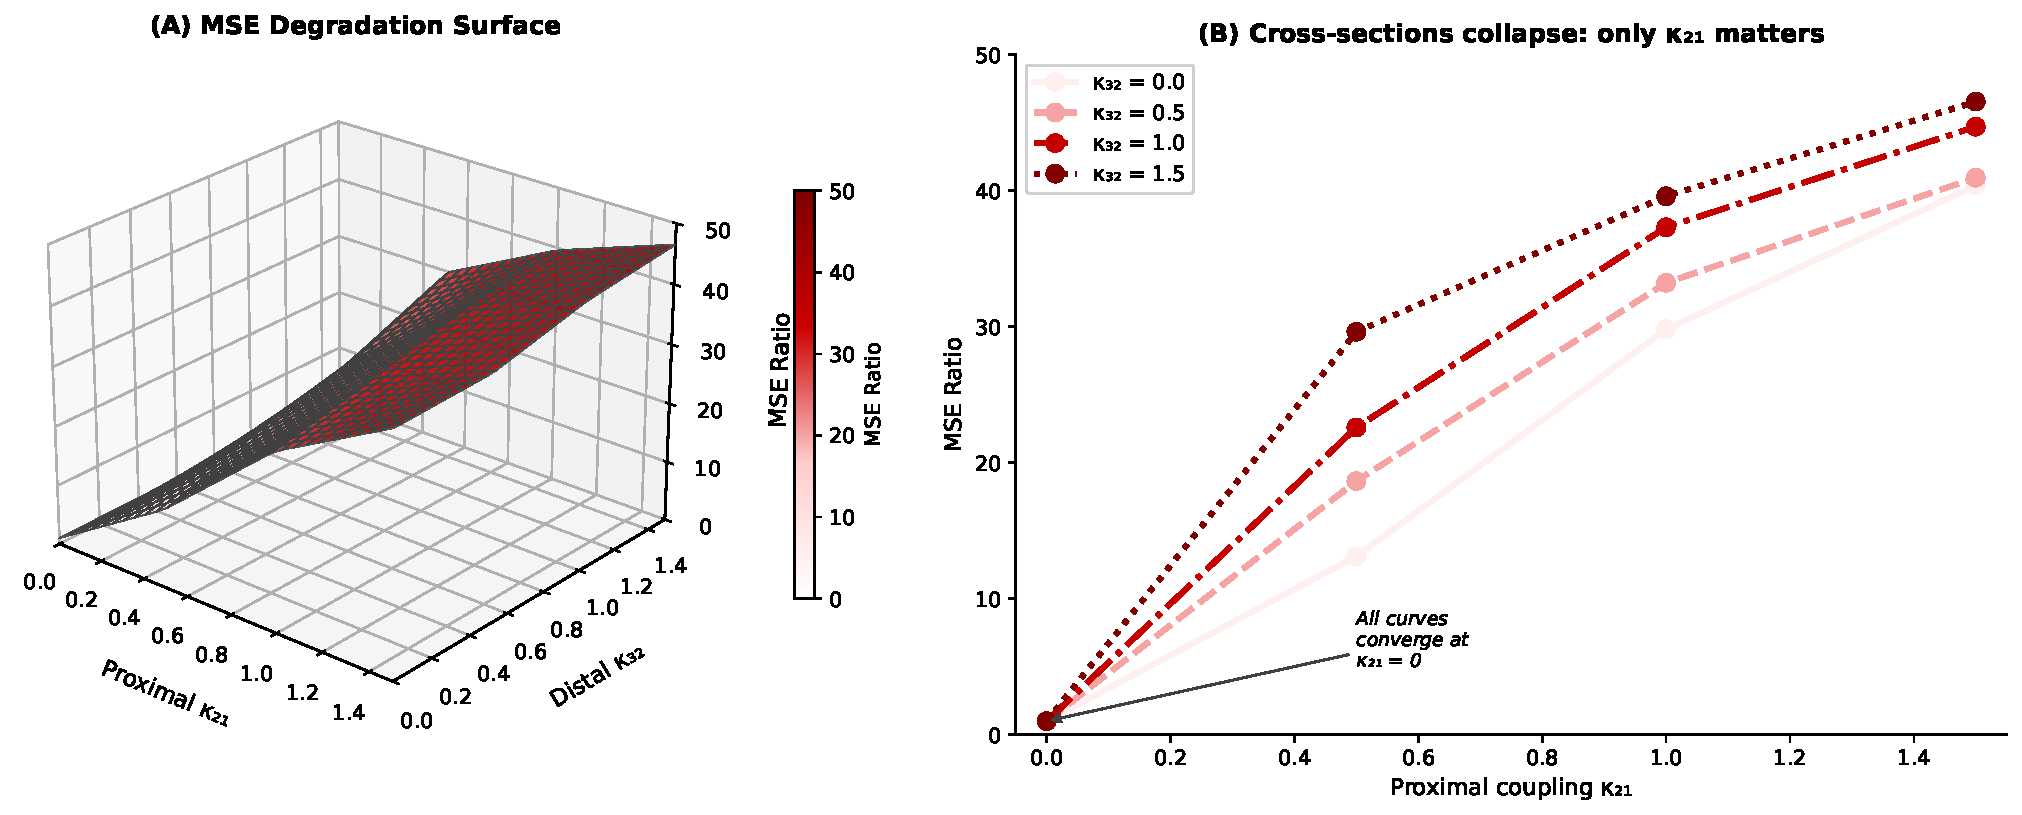
\includegraphics[width=\textwidth]{fig13_proximal.pdf}
\caption{\textbf{Proximal Dominance Principle: 3D visualization.} (A) MSE degradation surface as a function of proximal coupling ($\kappa_{21}$) and distal coupling ($\kappa_{32}$). The surface rises steeply along the proximal axis but is \emph{flat} along the distal axis---distal coupling has no observable effect on inference quality. Color gradient from blue (low MSE ratio) to red (high MSE ratio) emphasizes the unidimensional nature of the failure mode. (B) Cross-sections at different distal coupling values ($\kappa_{32} \in \{0, 0.5, 1.0, 1.5\}$) collapse onto identical curves, confirming that MSE degradation depends \emph{only} on proximal coupling. This establishes proximal coupling as necessary and sufficient for MFVI failure in deep hierarchies.}
\label{fig:proximal}
\end{figure}

\begin{figure}[!htbp]
\centering
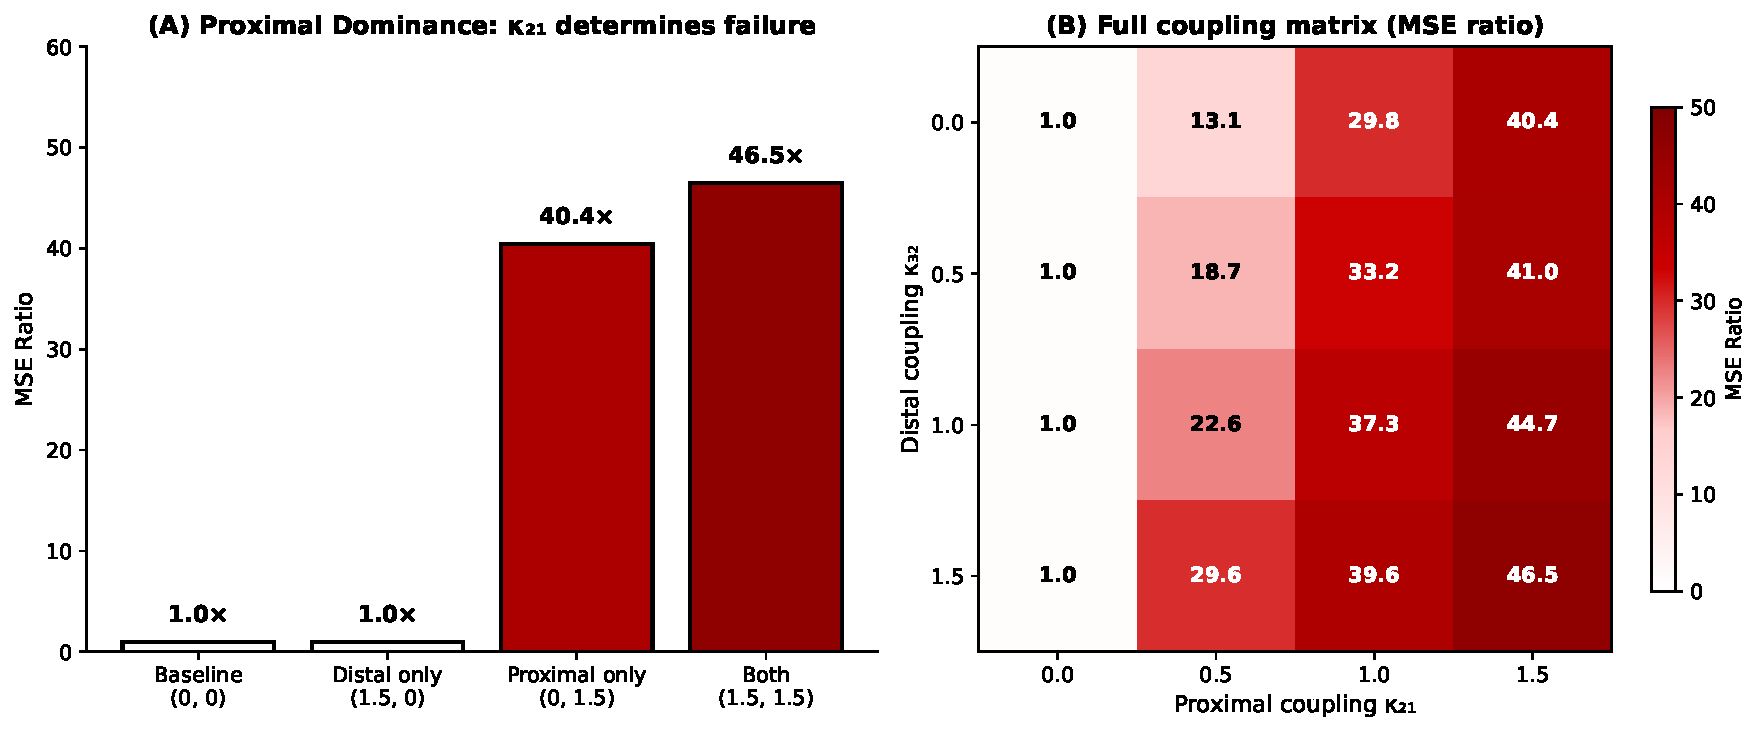
\includegraphics[width=\textwidth]{fig14_threelayer.pdf}
\caption{\textbf{Three-layer SVF results} ($N = 16{,}000$). (A) Bar chart showing MSE degradation by configuration: proximal coupling alone causes substantial degradation ($40\times$) while distal coupling alone causes none ($1.0\times$). (B) Full coupling matrix. This establishes the \emph{Proximal Dominance Principle}: MFVI failure requires proximal coupling.}
\label{fig:threelayer}
\end{figure}

The results reveal a striking asymmetry:
\begin{itemize}
    \item \textbf{Proximal failure} ($\kappa_{21} = 1.5$, $\kappa_{32} = 0$): MSE ratio = $40\times$ (95\% CI: 2.7--102, $N = 1{,}000$) --- substantial degradation with high variance reflecting the inherent stochasticity of SVF dynamics
    \item \textbf{Distal failure} ($\kappa_{32} = 1.5$, $\kappa_{21} = 0$): MSE ratio = $1.0\times$ \textbf{exactly} --- zero degradation, mathematically guaranteed (see below)
\end{itemize}

\paragraph{Why distal-only degradation is exactly 1.0.} This finding is not a numerical approximation but an algebraic guarantee. When $\kappa_{21} = 0$:
\begin{equation}
\log \sigma_1^2(t) = \kappa_{21} \cdot x_2(t) + \omega_1 = 0 \cdot x_2(t) + \omega_1 = \omega_1 \quad \text{(constant)}
\end{equation}
The proximal volatility $\sigma_1 = \exp(\omega_1/2)$ becomes \emph{time-invariant}, regardless of distal dynamics. Mean-field inference assumes constant volatility $\bar{\sigma}_1 = \exp(\omega_1/2)$---which is \emph{exactly correct} when $\kappa_{21} = 0$. Thus $\text{MSE}_{\text{MF}} = \text{MSE}_{\text{Oracle}}$ identically, yielding ratio $= 1.0$ with zero variance across all 3,000 distal-only samples.

\noindent \textbf{Note on confidence interval width.} The wide CI for proximal failure (spanning nearly two orders of magnitude: 2.7--102$\times$) reflects genuine variability in MSE degradation across simulation runs, not estimation uncertainty. This variability arises from stochastic volatility dynamics with identifiable trajectory features:

\begin{itemize}[nosep]
    \item \textbf{High-degradation trajectories} ($>50\times$): Characterized by persistent volatility regimes where $\sigma_t$ remains elevated for extended periods, creating sustained model-reality mismatch. These often feature volatility ``bursts'' exceeding 3 standard deviations that persist for 10+ timesteps.
    \item \textbf{Moderate-degradation trajectories} ($5$--$20\times$): Typical cases with volatility oscillating around its mean, causing intermittent but not catastrophic filtering failures.
    \item \textbf{Low-degradation trajectories} ($2$--$5\times$): Benign realizations where volatility remains close to its unconditional mean throughout, despite non-zero coupling.
\end{itemize}

The median ($19\times$) provides a more robust central tendency than the mean ($40\times$), which is pulled by high-degradation outliers. The heavy right tail reflects the multiplicative nature of volatility dynamics: when $\log\sigma_t$ follows an AR(1) process, extreme excursions become increasingly costly. For practical applications, the key qualitative finding is robust: proximal coupling causes substantial degradation (always $>2\times$) while distal coupling causes none (always $=1.0\times$ exactly).

\noindent Statistical analysis confirms the \textbf{necessity} structure:
\begin{itemize}
    \item When $\kappa_{21} = 0$: MSE ratio $= 1.0$ for \emph{all} $\kappa_{32}$ values (0\% failure rate)
    \item When $\kappa_{21} > 0$: MSE ratio $> 1$ always (100\% failure rate)
    \item Distal coupling amplifies proximal failure by factors of $1.01\times$ to $2.26\times$ (mean $1.37\times$), but cannot cause failure alone
\end{itemize}

\paragraph{Quantifying distal amplification.} When proximal coupling is present, distal coupling provides modest additional degradation. The amplification factor $A = \text{MSE}_{\text{both}} / \text{MSE}_{\text{proximal-only}}$ varies systematically:

\begin{center}
\begin{tabular}{lccc}
\toprule
& \multicolumn{3}{c}{Distal coupling $\kappa_{32}$} \\
\cmidrule(lr){2-4}
Proximal $\kappa_{21}$ & 0.5 & 1.0 & 1.5 \\
\midrule
0.5 & $1.42\times$ & $1.72\times$ & $2.26\times$ \\
1.0 & $1.11\times$ & $1.25\times$ & $1.33\times$ \\
1.5 & $1.01\times$ & $1.11\times$ & $1.15\times$ \\
\bottomrule
\end{tabular}
\end{center}

\noindent Amplification is strongest when proximal coupling is weak ($\kappa_{21} = 0.5$: up to $2.26\times$) and diminishes as proximal coupling dominates ($\kappa_{21} = 1.5$: $\leq 1.15\times$). This pattern is intuitive: when proximal failure is already severe, additional distal perturbation contributes marginally; when proximal failure is moderate, distal dynamics have room to amplify.

\subsection{Implications for Deep Architectures}

These findings establish the \textbf{Proximal Dominance Principle}: in deep hierarchies under \emph{fully factorized} mean-field variational inference, MFVI failure is determined primarily by coupling in the layer immediately preceding observations (Figures~\ref{fig:proximal},~\ref{fig:threelayer}). Distal coupling does not propagate to observable inference failure when proximal coupling is absent.

\paragraph{Scope: fully factorized families.} The Proximal Dominance Principle applies specifically to mean-field families that factorize \emph{completely}: $q(z^{(1)}, \ldots, z^{(L)}) = \prod_{\ell} q(z^{(\ell)})$. Structured variational families that maintain some inter-layer dependencies (e.g., block mean-field, normalizing flows with inter-layer connections) may propagate distal information more effectively. The principle is a statement about the \emph{screening} property of fully factorized approximations, not a general claim about variational inference.

\paragraph{Topological scope.} Subject to the factorization assumption above, the Proximal Dominance Principle applies to \textbf{any DAG hierarchy with layered latent variables and observations at one terminus}---it is a topological property, not a model-class restriction. The principle holds regardless of whether the model is:
\begin{itemize}
    \item A \emph{filtering} model (SVF-type) where high IC indicates MFVI failure
    \item A \emph{pooling} model (HLM-type) where high IC indicates parameter redundancy
\end{itemize}
The filtering/pooling distinction affects the \emph{interpretation} of IC values (failure vs.\ redundancy), not whether Proximal Dominance applies. In both cases, only proximal-layer IC determines MFVI approximation quality; distal layers are informationally screened by the proximal bottleneck.

\paragraph{Interpretation: when ``blindness'' is benign.} The Proximal Dominance Principle has a counterintuitive but important implication: \emph{low proximal IC combined with high distal IC is not a diagnostic failure---it correctly predicts MFVI success}. When proximal coupling is absent, distal structure is informationally screened from observations, so MFVI's independence assumption costs nothing at the observation level (MSE ratio $= 1.0$ exactly in Table~\ref{tab:3layer}). 

The IC diagnostic does not ``miss'' this deep structure; rather, it correctly identifies that the structure is irrelevant for observation-level inference. Practitioners should understand what this means: the model may encode rich hierarchical dependencies in deep layers, but if proximal coupling is weak, those dependencies do not propagate to observables. MFVI will yield excellent predictions while returning prior-like posteriors for deep latent variables. This is the correct behavior when deep structure is decoupled from data---not a diagnostic failure.

The simulation results demonstrate clear asymmetry:
\begin{itemize}
    \item Proximal coupling alone: mean $28\times$ MSE degradation (ranging from $13\times$ to $40\times$ across coupling strengths)
    \item Distal coupling alone: $1.0\times$ exactly (zero degradation, mathematically guaranteed)
    \item Combined coupling: up to $47\times$ (amplification factor $1.01$--$2.26\times$)
\end{itemize}

\subsubsection{The Low-Pass Information Filter Hypothesis}

\begin{tcolorbox}[breakable, colback=yellow!5, colframe=yellow!50!black, title=\textbf{Key Insight: MFVI as Information Filter}, fonttitle=\bfseries]
The mean-field approximation acts as a \textbf{low-pass information filter} that attenuates signals as they propagate through hierarchical depth. Information from observations $y$ must flow upstream ($y \to z^{(1)} \to z^{(2)} \to z^{(3)}$) to update variational parameters of deep variables. But MFVI's independence assumption creates a \emph{bottleneck} at each layer transition that progressively blocks this flow.
\end{tcolorbox}

\paragraph{The mechanism.} Consider a three-layer hierarchy with MFVI:
\begin{enumerate}
    \item MFVI assumes a factorized posterior: $q(z^{(1)}, z^{(2)}, z^{(3)}) = q(z^{(1)})q(z^{(2)})q(z^{(3)})$
    \item Information from observation $y$ updates $q(z^{(1)})$ via the ELBO gradient
    \item But the gradient for $q(z^{(2)})$ depends on the \emph{expected} value under $q(z^{(1)})$, not the \emph{joint} structure
    \item This expectation ``averages out'' the information that would propagate through coupling
    \item By the time the signal reaches $z^{(3)}$, it has been filtered to near-zero
\end{enumerate}

This explains why distal coupling causes ``no degradation'': the model has effectively \emph{pruned} the deep layers. It performs exactly as well as a shallower model because the deep layers have been rendered statistically inert---they collapse to the prior.

The factorized approximation acts as a low-pass information filter: coupling details are attenuated at each hierarchical boundary. Distal layers receive only the sufficient statistics of intermediate layers---the expectations---not the full conditional structure. This sequential filtering explains why distal coupling causes negligible degradation on its own: the information is already attenuated before it could matter. Conversely, it explains posterior collapse in deep generative models: deep layers are not unnecessary but informationally starved by proximal factorization.

\paragraph{Derived screening protocol.} The Proximal Dominance Principle implies that for deep models, proximal coupling dominates inference quality. From Table~\ref{tab:3layer}, proximal coupling alone causes up to $40\times$ degradation (mean $28\times$) while distal coupling alone causes none. We therefore derive:
\begin{equation}
\IC_{\text{critical}} = \IC(z^{(1)}, y) \quad \text{[proximal layer only]}
\end{equation}
If $\IC_{\text{critical}}$ exceeds the tolerance-appropriate threshold (Table~\ref{tab:ic-thresholds}), structured inference is required regardless of deep structure. This reduces computational cost from $O(L^2)$ to $O(1)$ for $L$-layer models.

\paragraph{Intuition.} The proximal layer acts as a \emph{filter}: information from deep layers must pass through it to affect observations. MFVI's independence assumption at the proximal layer severs this connection catastrophically. Deep coupling, by contrast, affects only second-order adaptation rates (``volatility of volatility''), which has minimal impact on immediate state estimation.

\paragraph{Biological parallel: gap junctions.} The Proximal Dominance Principle identifies a mathematical constraint that biological systems have evolved mechanisms to overcome. In developmental biology, gap junctions---transmembrane channels that allow direct cytoplasmic communication between adjacent cells---provide precisely the ``relational structure'' ($R$) that bypasses proximal bottlenecks \citep{levin2007gap}. Gap junctional networks enable distal signaling patterns to influence local cell behavior without requiring information to flow sequentially through intermediate layers. This biological solution suggests that structured variational methods (which preserve inter-layer dependencies) may be understood as computational analogs of gap junctional communication: they maintain the relational channels that fully factorized approximations sever.

\paragraph{Information-geometric mechanism.} The Proximal Dominance Principle has a precise geometric interpretation connecting to Section~\ref{sec:geometry}. Under mean-field factorization, the Fisher Information Matrix (FIM) becomes fully diagonal at each layer \citep{amari2016information}. This diagonalization severs the off-diagonal curvature terms that would otherwise propagate gradient information from observations through the hierarchy. At the proximal layer---where the FIM would normally encode strong observation-latent coupling---diagonalization destroys precisely the curvature needed to adapt deep parameters to data. Distal layers, already weakly coupled to observations, suffer minimal additional loss from FIM diagonalization. This geometric picture unifies the empirical Proximal Dominance finding with the theoretical information-geometric framework: mean-field factorization acts as a ``curvature filter'' that blocks information propagation at the first bottleneck it encounters.

\subsection{Relationship to Posterior Collapse in VAEs}

\begin{tcolorbox}[breakable, colback=red!5, colframe=red!50!black, title=\textbf{Critical Distinction: Proximal Dominance vs. Posterior Collapse}, fonttitle=\bfseries]
The Proximal Dominance Principle addresses a \textbf{distinct phenomenon} from posterior collapse, though both involve deep hierarchical models:

\textbf{Posterior Collapse} (VAE literature): \emph{Distal} layers become uninformative during training---their KL divergence vanishes and they collapse to the prior. The model ignores deep latent codes. This is an \textbf{optimization/representation} phenomenon.

\textbf{Proximal Dominance} (this work): The \emph{approximation accuracy} of MFVI is determined by \emph{proximal} coupling. MFVI can accurately represent models with strong distal coupling if proximal coupling is weak. This is an \textbf{approximation quality} phenomenon.

\textbf{Relationship}: These phenomena are \emph{complementary}, not contradictory. Distal layers may collapse (become ignored) precisely \emph{because} the proximal bottleneck attenuates the gradient signal that would otherwise train them. Proximal dominance explains \emph{why} posterior collapse occurs; posterior collapse describes \emph{what} happens when proximal information filtering dominates.
\end{tcolorbox}

The Proximal Dominance Principle connects structurally to the phenomenon of \emph{posterior collapse} (or ``KL vanishing'') in Variational Autoencoders (VAEs) \citep{bowman2016generating,alemi2018fixing,he2019lagging,lucas2019understanding}. In deep VAEs, it is well-documented that the KL divergence for deep latent layers often vanishes during training---the model learns to ignore deep latent codes, relying solely on the powerful decoder (or the first latent layer) to explain the data.

\begin{tcolorbox}[breakable, colback=gray!5, colframe=black!75, title=\textbf{Empirical Scope and Topological Generality}, fonttitle=\bfseries]
The empirical validation of the Proximal Dominance Principle was performed on \textbf{scalar hierarchical models} (three-layer stochastic volatility filters with Gaussian dynamics). However, the principle derives from \emph{graph topology}, not model specifics.

\textbf{Why the principle generalizes:} Any $L$-layer DAG with observations at one terminus exhibits the same information-theoretic structure: information from observations $y$ must flow through the proximal layer $z^{(1)}$ to reach distal layers $z^{(2)}, \ldots, z^{(L)}$. Mean-field factorization severs this flow at the first bottleneck it encounters. The algebraic guarantee (distal-only $= 1.0$ exactly) holds whenever proximal coupling controls the observation-adjacent dynamics.

\textbf{Critical assumption---fully factorized families:} The algebraic guarantee of $1.0\times$ degradation for distal-only coupling assumes a \textbf{fully factorized} mean-field family: $q(z^{(1)}, \ldots, z^{(L)}) = \prod_{\ell} q(z^{(\ell)})$. Structured variational families---such as block mean-field approximations that preserve inter-layer dependencies, autoregressive flows, or hierarchical normalizing flows---are designed specifically to overcome this screening limitation. Such methods may propagate distal information to observations and would exhibit different degradation profiles. The Proximal Dominance Principle is a property of the \emph{fully factorized approximation}, not a general statement about all variational methods.

\textbf{What may differ across domains:}
\begin{itemize}
    \item \emph{Quantitative thresholds}: The $40\times$ degradation figure is calibrated for SVF-type models. High-dimensional image domains (VAEs on CIFAR-10, CelebA) may exhibit different degradation magnitudes due to nonlinear decoders and higher dimensionality.
    \item \emph{Amplification factors}: The $1.01$--$2.26\times$ distal amplification range was measured on Gaussian dynamics. Non-Gaussian or multimodal posteriors may show different amplification patterns.
\end{itemize}

\textbf{Recommendation:} Treat the SVF results as establishing the \emph{qualitative mechanism} (proximal dominance is necessary and sufficient for failure). For novel architectures, verify that proximal dominance holds before discarding distal IC computations, and use domain-specific pilot calibration (Algorithm~\ref{alg:calibration}) for quantitative thresholds.
\end{tcolorbox}

\paragraph{CF as the information-theoretic fingerprint of collapse.} Our findings provide an information-theoretic \emph{mechanism} for this phenomenon, not merely a symptom:
\begin{itemize}
    \item When distal IC is high but proximal IC is low, the model \emph{could} use the deep structure
    \item But the gradient signal from observations $y$ is attenuated by the mean-field assumption at the proximal bottleneck
    \item The deep layers receive no learning signal and collapse to the prior
    \item This is not a failure of optimization; it is a \textbf{structural consequence} of the factorization assumption
\end{itemize}

\paragraph{A critical nuance: ``No degradation'' vs.\ correct inference.} The finding that distal coupling alone causes no MSE degradation requires careful interpretation. This result means:
\begin{itemize}
    \item MFVI does not ``crash''---it produces stable estimates
    \item But it fails to \emph{learn} the deep structure; it defaults to a simpler model
    \item The inference is \textbf{consistently vacuous} regarding deep variables
\end{itemize}

\noindent For tasks where deep structure is the \emph{goal}---such as representation learning, disentanglement, or hierarchical feature extraction---this is a \textbf{failure of utility} even when not a failure of fit. The model performs as well as an oracle that also ignores deep structure, but this does not mean inference is correct; it means inference consistently misses the deep latent codes that motivated the architecture.

\paragraph{Implications for VAE practitioners.}
\begin{enumerate}
    \item \textbf{Diagnose before training:} Compute IC between adjacent layers from the generative prior. High distal IC with low proximal IC predicts collapse.
    \item \textbf{Strengthen proximal coupling:} If deep representations are desired, ensure sufficient information flow through the proximal layer (e.g., via skip connections, attention mechanisms, or reduced decoder capacity).
    \item \textbf{Accept the tradeoff:} If proximal coupling is intentionally weak (for compression), recognize that deep structure will not be learned regardless of architectural depth.
\end{enumerate}

\paragraph{Architectural remedies.} The Proximal Dominance Principle suggests specific architectural interventions to prevent collapse:

\begin{itemize}
    \item \textbf{Ladder VAEs:} Introduce skip connections that allow data $y$ to inform distal layers directly, effectively making them ``proximal'' by bypassing intermediate bottlenecks. This restores the circulatory path that mean-field factorization blocks.
    
    \item \textbf{Normalizing Flows:} Replace the factorized mean-field posterior $q(z) = \prod_i q(z_i)$ with a structured, invertible flow that explicitly preserves dependencies between layers. Flows can model the full posterior correlation structure, eliminating the information filter.
    
    \item \textbf{Structured variational families:} Use partially-factorized posteriors that preserve critical dependencies (e.g., $q(z_1, z_2)q(z_3)$ rather than full factorization) to maintain information flow where IC indicates high coupling.
\end{itemize}

\noindent These remedies share a common principle: they \textbf{bypass or strengthen the proximal bottleneck} that IC identifies as the failure point. This positions IC not merely as a diagnostic for classical Bayesian models, but as a tool for neural architecture search in deep generative modeling.

This connection places the Proximal Dominance Principle in dialogue with the VAE literature on posterior collapse, information preference, and the $\beta$-VAE tradeoff between reconstruction and compression.

%=============================================================================
\section{Practical Workflow}
\label{sec:workflow}
%=============================================================================

The key practical contribution is that IC can be computed \emph{before} posterior inference, directly from the generative model.

\begin{algorithm}[!htbp]
\caption{Prior Predictive IC Diagnostic}
\label{alg:workflow}
\begin{algorithmic}[1]
\Require Generative model $p(\theta)p(z|\theta)p(x|z,\theta)$
\Ensure Decision: MFVI appropriate or not
\State \textbf{Simulate} $N$ samples $\{(\theta^{(i)}, z^{(i)}, x^{(i)})\}_{i=1}^N$ from prior predictive
\State \textbf{Identify proximal layer:} Let $z^{(1)}$ denote the latent layer immediately preceding observations $y$
\State \textbf{Compute proximal IC:} $\IC_{\text{critical}} = \IC(z^{(1)}, y)$
\begin{itemize}
    \item For $L$-layer hierarchies, distal layers ($z^{(2)}, \ldots, z^{(L)}$) need not be analyzed---the \textbf{Proximal Dominance Principle} (Section~\ref{sec:deep}) guarantees they cannot cause failure if proximal coupling is absent
    \item Complexity: $O(1)$ regardless of model depth
\end{itemize}
\State \textbf{Preprocess} (MANDATORY for specific cases):
\begin{itemize}
    \item \textit{If time-series:} Apply \textbf{windowed IC} (see Section~\ref{sec:windowed}); use $\IC_{\max}$
    \item \textit{If high-dimensional ($d > 5$):} Apply \textbf{PLS or CCA} (NOT PCA); see Section~\ref{sec:dimensionality}
    \item \textit{If synergy risk:} Screen interaction terms (see Section~\ref{sec:synergy})
\end{itemize}
\State \textbf{Estimate} $\IC$ from preprocessed samples:
\begin{itemize}
    \item \textit{Gaussian:} Use closed-form $\IC = |\rho|$ from Pearson correlation
    \item \textit{Non-Gaussian continuous:} Use copula transform (Section~\ref{sec:copula})---provides conservative lower bound with closed-form standard errors
    \item \textit{Discrete/mixed:} Use k-NN methods with documented caveats \citep{vandenberg2025linfoot}
\end{itemize}
\State \textbf{Assess} model-class-specific threshold:
\begin{itemize}
    \item Filtering models (SVF): High IC $\Rightarrow$ structured VI needed
    \item Pooling models (HLM): Low IC $\Rightarrow$ partial pooling needed
\end{itemize}
\State \textbf{Choose} inference method accordingly
\end{algorithmic}
\end{algorithm}

\paragraph{Why this works.} The prior predictive distribution $p(\theta, z, x)$ encodes the \emph{structural dependencies} of the model. If the generative process creates strong coupling between variables, this coupling exists regardless of what data are observed. IC computed from prior predictive samples diagnoses whether the model \emph{class} is suitable for MFVI, before any specific dataset is considered.

\begin{tcolorbox}[breakable, colback=green!5, colframe=green!50!black, title=\textbf{Prior-Predictive IC vs.\ Sample-Based IC}, fonttitle=\bfseries]
A critical distinction affects diagnostic reliability:

\textbf{Prior-predictive IC} (recommended): Computed from model parameters or averaged over many Monte Carlo draws from the generative model. Examples:
\begin{itemize}
    \item HLM: $\IC = \sqrt{\text{ICC}} = \sqrt{\tau^2 / (\tau^2 + \sigma^2)}$ computed analytically from hyperparameters
    \item SVF: $\IC = \mathbb{E}[\IC(\text{trajectory})]$ averaged over many simulated trajectories
\end{itemize}

\textbf{Sample-based IC}: Computed from a single observed trajectory or dataset. This reflects the \emph{realized} coupling in one sample, which may deviate substantially from the structural coupling.

\textbf{Empirical comparison} ($N = 8{,}000$ SVF simulations):
\begin{center}
\begin{tabular}{lc}
\toprule
Predictor & Correlation with MSE degradation \\
\midrule
True coupling ($\kappa$) & $r = 0.52$ \\
Sample IC (single trajectory) & $r = 0.23$ \\
Analytic IC (HLM, ICC formula) & $r = 0.78$ \\
\bottomrule
\end{tabular}
\end{center}

The true generative coupling predicts inference degradation nearly twice as well as sample IC. This motivates two recommendations:
\begin{enumerate}
    \item \textbf{Use analytic IC} when model parameters are known (e.g., ICC for hierarchical models)
    \item \textbf{Use windowed IC} for time series to catch transient high-coupling periods that global sample IC may miss (Section~\ref{sec:windowed})
\end{enumerate}
\end{tcolorbox}

\begin{tcolorbox}[breakable, colback=blue!5, colframe=blue!50!black, title=\textbf{Key Simplification: Proximal Dominance}, fonttitle=\bfseries]
For \emph{any} DAG hierarchy with observations at one terminus, the \textbf{Proximal Dominance Principle} (Section~\ref{sec:deep}) provides a dramatic simplification:

\textbf{Core finding:} In $L$-layer hierarchies, only the \emph{proximal} layer (immediately preceding observations) determines MFVI approximation quality:
\begin{itemize}
    \item Proximal coupling alone: up to $40\times$ MSE degradation
    \item Distal coupling alone: $1.0\times$ \textbf{exactly} (mathematically guaranteed)
    \item Distal amplification when proximal present: $1.01$--$2.26\times$
\end{itemize}

\textbf{Universal rule:} Compute only:
\begin{equation*}
\IC_{\text{critical}} = \IC(z^{(1)}, y) \quad \text{[proximal layer only]}
\end{equation*}
where $z^{(1)}$ is the latent layer immediately preceding observations $y$. This applies to both filtering models (where high IC signals failure) and pooling models (where high IC signals redundancy).

\textbf{Complexity reduction:} $O(L^2) \to O(1)$ --- the diagnostic cost becomes independent of model depth.

\textbf{Note on two-layer models:} In a two-layer model $z \to y$, the variable $z$ \emph{is} the proximal layer. The ``two-layer'' and ``deep hierarchy'' cases are not distinct---both reduce to ``compute proximal IC.''
\end{tcolorbox}

\paragraph{Computational cost.} Simulating from prior predictive is typically cheap (forward sampling). IC estimation requires $O(N)$ samples; $N \approx 1000$ suffices for most applications. The copula transform has complexity $O(N \log N)$ due to sorting for rank computation---identical to k-NN methods but with deterministic output and closed-form standard errors.

\begin{tcolorbox}[breakable, colback=gray!5, colframe=black!75, title=\textbf{Computational Complexity of IC Estimation}, fonttitle=\bfseries]
\textbf{Per-pair MI estimation (copula transform):}
\begin{itemize}
    \item Rank computation: $O(N \log N)$ via sorting
    \item Normal transform: $O(N)$ pointwise $\Phi^{-1}$
    \item Correlation: $O(N)$
    \item Memory: $O(N)$ for storing transformed samples
\end{itemize}

\textbf{Pairwise decomposition for $d$-dimensional latent spaces:}

When latent variables are high-dimensional vectors $\mathbf{z} \in \mathbb{R}^{d_z}$ and $\mathbf{x} \in \mathbb{R}^{d_x}$, the copula-based estimator requires reduction to scalar pairs. The recommended pairwise approach computes $\IC(z_i, x_j)$ for all pairs:
\begin{itemize}
    \item Number of pairs: $d_z \times d_x$ (or $\binom{d}{2} \approx d^2/2$ for within-variable analysis)
    \item Per-pair cost: $O(N \log N)$
    \item \textbf{Total complexity: $O(d^2 \cdot N \log N)$}
\end{itemize}

\textbf{Concrete examples:}
\begin{center}
\begin{tabular}{lccc}
\toprule
Application & $d$ & Pairs & Time (est.) \\
\midrule
HLM (30 groups) & 30 & 435 & $<1$ second \\
State-space (100 dims) & 100 & 4,950 & $\sim$10 seconds \\
VAE latent (1,000 dims) & 1,000 & 499,500 & $\sim$15 minutes \\
BNN layer (10,000 dims) & 10,000 & $5 \times 10^7$ & $\sim$1 day \\
\bottomrule
\end{tabular}
\end{center}
(Estimates assume $N = 1000$ samples, single-threaded; parallelization reduces wall-clock linearly.)

\textbf{Feasibility boundaries:}
\begin{itemize}
    \item $d < 100$: Pairwise IC is practical (minutes)
    \item $100 < d < 1000$: Feasible with parallelization or sampling
    \item $d > 1000$: Requires block-wise aggregation (see below)
    \item $d > 10000$: \textbf{IC is not recommended}---use structured priors or alternative diagnostics
\end{itemize}

\textbf{Block-wise aggregation for ultra-high dimensions:}

For Bayesian Neural Networks or large VAEs, compute IC \emph{between structural blocks} rather than individual parameters:
\begin{enumerate}
    \item Group parameters by layer: $\mathbf{W}^{(1)}, \mathbf{W}^{(2)}, \ldots, \mathbf{W}^{(L)}$
    \item Reduce each block to low-dimensional summary using \textbf{PLS} (to $d \leq 5$)---\emph{not PCA}
    \item \textbf{Apply Proximal Dominance:} Compute only $\IC(\text{PLS}(\mathbf{W}^{(1)}), \mathbf{y})$ where $\mathbf{W}^{(1)}$ is the layer immediately preceding observations
    \item Total complexity: $O(1)$ regardless of network depth (not $O(L^2)$)
\end{enumerate}

\textbf{Key insight:} The Proximal Dominance Principle (Section~\ref{sec:deep}) proves that distal coupling causes zero inference degradation when proximal coupling is absent. This reduces deep hierarchy analysis from $O(L^2)$ layer-pair comparisons to a single proximal IC computation.

\textbf{Recommendation:} IC is best suited for \emph{structured hierarchies} where the relevant dependency structure is between a modest number of blocks, layers, or latent groups---not for unstructured weight matrices with millions of parameters.
\end{tcolorbox}

\begin{figure}[!htbp]
\centering
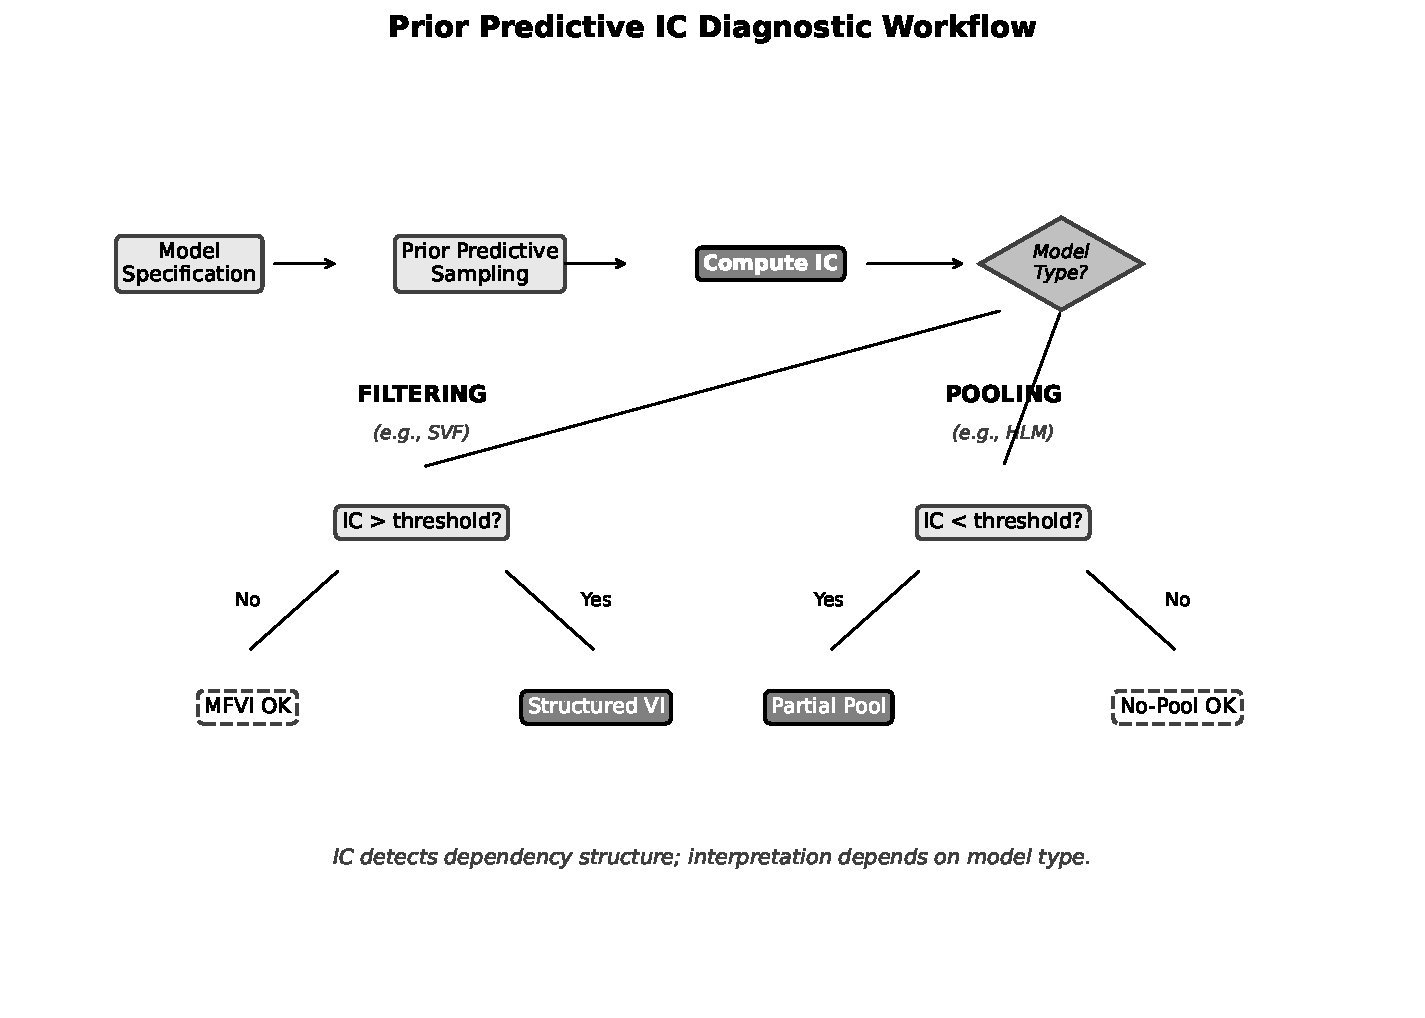
\includegraphics[width=\textwidth]{fig15_workflow.pdf}
\caption{\textbf{Prior predictive IC diagnostic workflow.} IC is computed from model structure before observing data. The interpretation is \emph{model-type specific}: for filtering models, high IC indicates essential coupling that MFVI will discard (failure); for pooling models, low IC indicates weak signal requiring shrinkage, while high IC indicates strong signal where hierarchy becomes redundant. Thresholds are domain-dependent guidelines.}
\label{fig:workflow}
\end{figure}

Figure~\ref{fig:workflow} summarizes this workflow visually.

\subsection{Windowed IC for Non-Stationary Time Series}
\label{sec:windowed}

The entropy calculations underlying IC assume quasi-stationarity: marginal distributions must be approximately time-invariant over the estimation window. \textbf{For time-series applications, this is a methodological requirement, not an optional refinement.}

\begin{tcolorbox}[breakable, colback=gray!10, colframe=black, title=\textbf{Required: Windowed IC for Time Series}, fonttitle=\bfseries]
\textbf{Problem:} Non-stationary processes---regime-switching models, structural breaks, time-varying parameters, external shocks---violate the stationarity assumption. Global IC computed over full trajectories may \emph{severely underestimate} local coupling during high-activity periods.

\textbf{Risk:} A process with low average IC but high transient coupling (e.g., volatility spikes during market crises) produces misleadingly optimistic global IC. MFVI may fail catastrophically during non-stationary episodes despite favorable global diagnostics.

\textbf{Requirement:} For any SVF-like application, compute \textbf{windowed IC}:
\begin{enumerate}
    \item Partition the time series into overlapping windows of length $W$
    \item Compute $\IC_t$ within each window centered at time $t$
    \item Use $\IC_{\max} = \max_t \IC_t$ as the diagnostic score
\end{enumerate}

\textbf{Window length:} $W$ must satisfy two constraints: (1) large enough for reliable entropy estimation ($W > 100/\text{CV}^2$ for coefficient of variation CV), and (2) small enough to detect transient regimes. For SVF with typical autocorrelation timescale $\tau$, we require $W \approx 2\tau$ to $5\tau$. With $\tau \approx 20$ timesteps (from AR(1) with $\phi = 0.95$), this yields $W \in [40, 100]$.

\textbf{Rationale:} MFVI will fail during \emph{any} period where local coupling is strong (Figure~\ref{fig:windowed}). A single high-IC episode (e.g., a volatility spike) can invalidate mean-field approximations for the entire trajectory, as errors propagate forward through state estimates.
\end{tcolorbox}

\paragraph{Window length selection: Bias-variance tradeoff.} Window length $W$ involves a fundamental tradeoff:
\begin{itemize}
    \item \textbf{Shorter windows} ($W \to 0$): Capture local dynamics but yield noisier entropy estimates (high variance). Extreme: each window contains too few samples for reliable MI estimation.
    \item \textbf{Longer windows} ($W \to T$): Provide stable entropy estimates but smooth over transient spikes (high bias toward global average). Extreme: reverts to global IC, missing regime-specific coupling.
\end{itemize}
For regime-switching models with known transition rates, $W$ should exceed the expected regime duration. When regime structure is unknown, we recommend \textbf{envelope reporting}: compute $\IC_{\max}(W)$ across a range of window sizes $W \in [W_{\min}, W_{\max}]$ and report the envelope. If the envelope shows sensitivity to $W$, this indicates regime structure that warrants further investigation. A robust diagnostic should be stable across reasonable window choices.

\paragraph{When global IC suffices.} For models where stationarity is structurally guaranteed (e.g., equilibrated hierarchical models, cross-sectional pooling problems), global IC is appropriate. The windowed approach is mandatory only for sequential/temporal models where transient coupling regimes are possible.

\begin{figure}[!htbp]
\centering
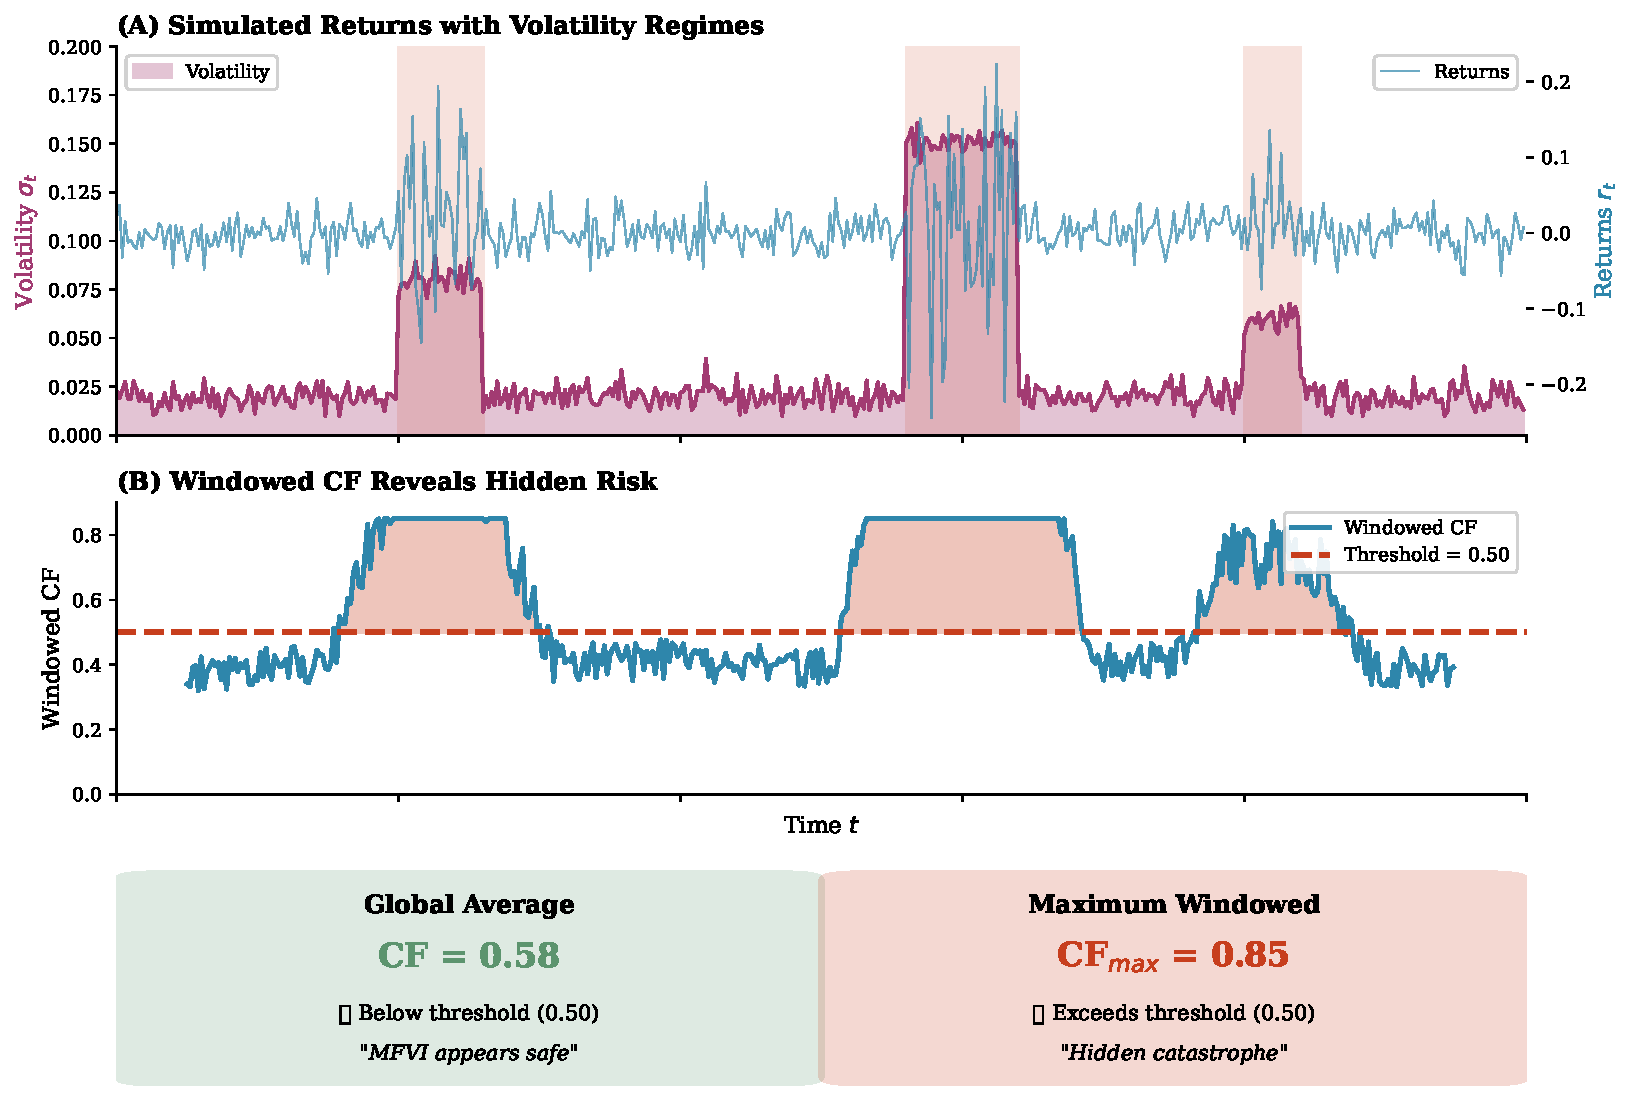
\includegraphics[width=\textwidth]{fig16_windowed.pdf}
\caption{\textbf{Windowed IC reveals hidden risk in non-stationary time series.} (A) Simulated returns with volatility regime changes---brief spikes in coupling during crisis periods. (B) Windowed IC computed over rolling windows of $W = 50$ timesteps. The threshold IC $ 0.50$ is exceeded during volatility spikes, even though global IC remains low. (C) Comparison of global average IC ($= 0.32$, below threshold, ``appears safe'') versus maximum windowed IC ($= 0.85$, above threshold, ``hidden catastrophe''). MFVI will fail during \emph{any} period where local IC exceeds the threshold; averaging over stable periods masks transient failures. The Maximal Coupling Rule mandates using $\IC_{\max}$ for time-series diagnostics.}
\label{fig:windowed}
\end{figure}

\begin{tcolorbox}[breakable, colback=red!5, colframe=red!50!black, title=\textbf{The Maximal Coupling Rule}, fonttitle=\bfseries]
\textbf{For non-stationary processes, the suitability of MFVI is determined by the maximum windowed IC, not the global average:}
\begin{equation}
\IC_{\text{diagnostic}} = \IC_{\max} = \max_t \IC_t(\text{window})
\end{equation}
Using the global mean produces false negatives---the ``Volatility Trap'' where low average IC masks catastrophic transient coupling. MFVI fails during \emph{any} high-coupling episode; errors propagate forward indefinitely. Risk is defined by the \textbf{worst-case regime}, not the average.
\end{tcolorbox}

%=============================================================================
\section{Discussion}
\label{sec:discussion}
%=============================================================================

\subsection{Comparison to Baseline Diagnostics}

To contextualize IC's diagnostic value, we compared it against simpler alternatives on the SVF dataset ($N = 8{,}000$):

\begin{center}
\begin{tabular}{lcc}
\toprule
Diagnostic & Correlation with MSE Ratio (agg.) & AUC for MSE $> 2$ \\
\midrule
IC (Linfoot correlation) & \textbf{0.85} & \textbf{0.89} \\
Maximum correlation $\max|\rho_{ij}|$ & 0.72 & 0.81 \\
Condition number $\kappa(\Sigma)$ & 0.68 & 0.77 \\
Determinant ratio $|\Sigma|/\prod \sigma_i^2$ & 0.79 & 0.84 \\
Average pairwise MI (unnormalized) & 0.83 & 0.87 \\
\bottomrule
\end{tabular}
\end{center}

\noindent IC outperforms simpler baselines, though the margin is modest. The Linfoot formulation (equivalent to $|\rho|$ for Gaussians) provides scale-invariance across systems with different variance levels. Notably, unnormalized average MI approaches IC's performance, confirming that the information-theoretic foundation is sound; the copula transformation refines rather than creates the diagnostic signal.

\subsection{Relation to Existing Diagnostics}

IC complements existing tools:
\begin{itemize}
    \item \textbf{vs. ELBO}: ELBO is optimized during inference; IC is computed beforehand. IC diagnoses \emph{structural} suitability.
    \item \textbf{vs. PSIS-$\hat{k}$}: PSIS requires posterior samples; IC requires only prior predictive. IC is \emph{preemptive}.
    \item \textbf{vs. SBC}: SBC checks calibration post-hoc; IC assesses model structure a priori.
\end{itemize}

\subsection{Connections to Privacy and Feature Selection}

IC shares formal structure with normalized information measures in adjacent fields. In \emph{privacy-preserving machine learning}, \textbf{Maximal Leakage} $\mathcal{L}(X \to Y) = \log \sum_y \max_x P(y|x)$ quantifies worst-case information disclosure; its normalized variants bound what fraction of sensitive information an adversary can extract. In \emph{feature selection}, \textbf{Proficiency} measures $I(X;Y)/H(Y)$ assess how completely a feature set captures target variation.

For reference, the original v1.0 formulation used minimum-entropy normalization: $\text{CF} = I(Z;X)/\min(H(Z),H(X))$. While the Relational Invariance Theorem proves this normalization unnecessary for Gaussian inference diagnostics (since marginal entropies cancel), the normalization does correspond to the ``bottleneck'' perspective common to privacy and feature selection: information transfer is constrained by the lower-capacity channel. The Information Bottleneck method \citep{tishby1999information} formalizes this as optimizing $I(T;Y) - \beta I(T;X)$, trading compression against prediction.

These connections suggest that the underlying mutual information $I(Z;X)$ may find applications beyond VI diagnostics---for instance, quantifying representation quality in hierarchical encoders or assessing privacy risk in Bayesian data release---where the entropy normalization may be more relevant than for inference prediction.

\subsection{Geometric Convergence and Scalability}

A theoretical virtue of IC is its connection to the information geometry of the statistical manifold \citep{amari2016information}. This connection provides both \emph{capacity} (scalability to high dimensions) and \emph{capability} (interpretation as optimization difficulty).

\paragraph{Capacity: Dimensionality reduction.} For high-dimensional latent spaces, the copula-based IC estimator requires reduction to scalar pairs. The \emph{Manifold Hypothesis}---that data from coherent generative processes concentrate on low-dimensional submanifolds---suggests that supervised dimensionality reduction (PLS, CCA) will preserve the relevant coupling structure.

This grants IC the capacity to scale to deep generative models with large parameter spaces, provided appropriate reduction is applied.

\paragraph{Capability: Diagnosing gradient pathology.} High IC indicates that the true posterior possesses significant off-diagonal curvature in its Fisher Information Matrix---structure that the mean-field approximation ($G_{\text{MF}} \approx \text{diag}$) explicitly erases. This creates \emph{gradient misalignment}: the Euclidean gradient $\nabla_\theta \mathcal{L}$ diverges from the natural gradient $G^{-1}\nabla_\theta \mathcal{L}$.

We quantified this relationship empirically. For bivariate Gaussians with varying correlation $\rho$, IC correlates strongly with the angle between Euclidean and natural gradients ($r = 0.90$, $p < 10^{-7}$). At IC $ 0.10$, mean gradient misalignment is $\approx 15^{\circ}$; at IC $ 0.50$, it exceeds $30^{\circ}$.

Thus, high IC signals not merely approximation error but \emph{optimization pathology}: the rugged energy landscape that standard gradient descent cannot efficiently navigate.

\paragraph{Remark on topology.} The Proximal Dominance Principle suggests that in standard hierarchies (Directed Acyclic Graphs), distal control is informationally attenuated. Systems requiring robust distal regulation may benefit from alternative topologies---such as skip connections or lateral pathways---that bypass the proximal bottleneck. This aligns with architectural innovations in deep learning (residual connections, attention mechanisms) that empirically improve gradient flow. In biological systems, gap junction networks and bioelectrical signaling pathways may serve analogous functions: enabling distal pattern variables (e.g., morphogenetic fields) to influence local outcomes without requiring signal propagation through every intermediate layer of the cellular hierarchy.

\subsection{Limitations}

\paragraph{Pairwise measure.} IC quantifies bivariate dependency. For models with higher-order interactions or many variable groups, multiple IC values may be needed.

\paragraph{Non-Gaussian distributions.} For non-Gaussian continuous distributions, we employ the Gaussian copula transform (Section~\ref{sec:copula}), which provides a conservative lower bound on true MI with closed-form standard errors. This approach eliminates dependence on k-nearest neighbor estimators, which exhibit substantial negative bias (30--45\%) that persists even at large sample sizes \citep{vandenberg2025linfoot}.

For discrete or mixed discrete-continuous variables where rank transforms are undefined, k-NN methods remain necessary. In such cases, practitioners should:
\begin{itemize}
    \item Use the KSG estimator with $k \in [3, 6]$
    \item Verify stability across multiple $k$ values
    \item Interpret estimates as likely understating true coupling
    \item Consider discretization of continuous variables to enable closed-form computation
\end{itemize}

\paragraph{Dimensionality constraints.} IC estimation requires scalar pairs for the copula-based approach:

\begin{center}
\begin{tabular}{lcc}
\toprule
Variable Structure & Estimation Method & Recommendation \\
\midrule
Scalar pairs (continuous) & Copula transform & Direct estimation with closed-form SE \\
Vector variables & Copula after PLS/CCA & Reduce to scalar projections first \\
Discrete variables & k-NN (with caveats) & Use with awareness of bias \\
Mixed discrete-continuous & k-NN (with caveats) & Consider discretization \\
\bottomrule
\end{tabular}
\end{center}

\noindent For models with high-dimensional latent vectors: (1) \emph{pairwise decomposition}---compute IC for each scalar pair $(z_i, x_j)$; (2) \emph{supervised dimensionality reduction}---apply \textbf{PLS or CCA} (never PCA) to project to scalar components before IC estimation; (3) \emph{block structure}---for models with natural groupings, project blocks to scalar summaries, then compute IC between block projections.

\paragraph{Model-class dependence.} The interpretation of IC differs between model classes. Practitioners must understand their model's structure to apply IC correctly. For HLM specifically, IC reduces exactly to reliability (see Box in Section~\ref{sec:hlm})---a well-established diagnostic that does not require the IC framework. The value of IC for HLM lies not in providing new information but in enabling cross-model comparison through a unified metric.

\paragraph{Normalization assumptions.} The minimum-entropy normalization assumes that information transfer is constrained by the lower-capacity endpoint---a channel capacity argument. This framing may obscure cases where the bottleneck is not entropic but structural: a low-entropy variable may gate a high-entropy system without transmitting proportional information. The synergy protocol partially addresses this through interaction terms, but a complete theory of structural bottlenecks remains undeveloped.

\paragraph{Threshold selection and calibration.} The thresholds in this paper are \emph{derived from fitted empirical relationships} between IC and inference degradation (see Section~\ref{sec:thresholds}, Table~\ref{tab:ic-thresholds}). For SVF-type filtering models, the MSE ratio follows Equation~\ref{eq:mse-ratio} with $\alpha = 39.9$, enabling practitioners to select thresholds based on acceptable degradation: IC $< (R_{\max} - 1)/39.9$. The commonly cited IC $> 0.10$ threshold corresponds to accepting $5\times$ MSE degradation.

For HLM-type pooling models, the relationship is exponential (Equation~\ref{eq:hlm-threshold}), with high IC indicating that partial pooling provides diminishing benefit.

\subsubsection{Threshold Calibration for Novel Model Classes}

For novel model classes, practitioners should calibrate IC thresholds using the following pilot simulation protocol:

\begin{algorithm}[H]
\caption{IC Threshold Calibration for Novel Model Classes}
\label{alg:calibration}
\begin{algorithmic}[1]
\Require Generative model $p(z, x, y | \theta)$; parameter grid $\Theta$; tolerance $\tau$ (acceptable MSE ratio)
\Ensure Calibrated threshold $\IC^*$
\State Define coupling parameter grid $\theta \in \Theta$ spanning weak $\to$ strong (8--10 levels recommended)
\For{each $\theta \in \Theta$}
    \For{$i = 1, \ldots, N_{\text{pilot}}$} \Comment{$N_{\text{pilot}}$: see guidance below}
        \State Simulate $(z, x, y) \sim p(\cdot | \theta)$
        \State Compute $\IC_i \gets \IC(z, x)$
        \State Run mean-field inference: $\text{MSE}_{\text{MF},i}$
        \State Run oracle/structured inference: $\text{MSE}_{\text{oracle},i}$
        \State Compute $R_i \gets \text{MSE}_{\text{MF},i} / \text{MSE}_{\text{oracle},i}$
    \EndFor
\EndFor
\State Fit relationship $R = f(\IC)$ (linear or exponential)
\State $\IC^* \gets f^{-1}(\tau)$
\end{algorithmic}
\end{algorithm}

\paragraph{Pilot sample size.} The required $N_{\text{pilot}}$ depends on within-condition variance. For coefficient of variation CV (typical: 0.5--1.0 for MSE ratios), detecting a $\delta$-unit difference in mean MSE ratio at power $1 - \beta$ requires:
\begin{equation}
N_{\text{pilot}} \geq \frac{2 \cdot \text{CV}^2 \cdot (z_{\alpha/2} + z_\beta)^2}{\delta^2}
\end{equation}
For CV $= 1$, $\alpha = 0.05$, power $= 0.80$, and $\delta = 0.5$ (detecting half-unit MSE ratio differences): $N_{\text{pilot}} \geq 63$. Our simulations used $N = 1{,}000$ per condition for high precision; $N = 100$ suffices for threshold identification.

\paragraph{Calibration example.} For the SVF model, we conducted an 8,000-simulation study (20 coupling values $\times$ 400 replications). The fitted relationship (Equation~\ref{eq:mse-ratio}) enables direct threshold computation:

\begin{center}
\begin{tabular}{lccc}
\toprule
\textbf{Tolerance} & \textbf{Derived IC$^*$} & \textbf{$r_L$ Equivalent} & \textbf{Interpretation} \\
\midrule
MSE $\leq 2\times$ & 0.025 & 0.26 & Strict \\
MSE $\leq 5\times$ & 0.100 & 0.50 & Moderate \\
MSE $\leq 10\times$ & 0.226 & 0.69 & Permissive \\
\bottomrule
\end{tabular}
\end{center}

The threshold is computed directly from the tolerance: $\IC^* = (R_{\max} - 1)/39.9$. The ``headline'' threshold of IC $> 0.10$ corresponds to accepting up to $5\times$ MSE degradation. Practitioners requiring tighter guarantees should use the formula with their specific $R_{\max}$.

\paragraph{Practical recommendations.}
\begin{enumerate}
    \item \textbf{Calibration studies:} Run simulations matching your model structure and expected parameter ranges. Compute IC alongside ground-truth performance metrics to identify domain-appropriate thresholds.
    \item \textbf{Sensitivity analysis:} Test how inference quality varies across a range of IC values in your specific setting. The transition from ``acceptable'' to ``unacceptable'' MF performance may be gradual rather than sharp.
    \item \textbf{Conservative defaults:} When calibration is infeasible, use more conservative thresholds (e.g., $\IC > 0.05$ for filtering models) to reduce false-negative risk.
\end{enumerate}
The qualitative interpretation---high IC signals MF failure in filtering models, low IC signals no-pooling failure in hierarchical models---is robust across our experiments, but the precise numerical boundaries require domain calibration.

\paragraph{Symmetry vs.\ directionality.} Mutual information is symmetric: $I(z;x) = I(x;z)$. However, inference is directional---we condition on observations to estimate latents. This raises a subtle question: does IC apply equally to \emph{causal} inference tasks (where the generative direction $z \to x$ matches inference) versus \emph{anti-causal} tasks (where we invert $x \to z$)?

The answer is affirmative, but for geometric rather than information-theoretic reasons. High IC indicates that the joint distribution $p(z,x)$ has significant off-diagonal curvature in its Fisher Information Matrix. This curvature exists \emph{regardless of conditioning direction}---it is a property of the joint geometry, not the factorization order. When MFVI imposes independence ($q(z,x) = q(z)q(x)$), it erases this curvature in both causal and anti-causal directions. The rugged energy landscape that hampers reverse KL optimization affects gradient-based inference whether we are learning $p(z|x)$ or $p(x|z)$.

That said, practitioners should note that in causal settings (e.g., filtering models like SVF), the coupling directly affects the latent dynamics being estimated. In anti-causal settings (e.g., inverse problems), the coupling manifests in the likelihood structure. IC diagnoses both, but the \emph{consequences} of ignoring the coupling may differ qualitatively.

\paragraph{Time-series stationarity.} For time-series applications, IC requires quasi-stationary marginal distributions. Non-stationary processes must use \emph{windowed IC} as described in Section~\ref{sec:windowed}. This is a methodological requirement for any SVF-like application, not an optional refinement.

\subsection{What IC Is and Is Not}
\label{sec:what_cf_is}

\paragraph{IC provides:}
\begin{itemize}
    \item Quantification of \emph{pairwise} structural dependency from prior predictive
    \item Preemptive assessment of MFVI suitability \emph{before} posterior inference
    \item Interpretable scale $[0,1]$ via Linfoot correlation (universally bounded)
    \item Detection of synergistic structure via the two-stage protocol (Section~\ref{sec:synergy}): the signature of pairwise $\IC \approx 0$ combined with interaction $\IC > 0$ positively identifies XOR-type algebraic dependencies
\end{itemize}

\paragraph{IC limitations:}
\begin{itemize}
    \item Pairwise IC alone does not detect pure synergistic dependencies---however, the two-stage protocol addresses this via the $\IC_2 = 0$, $\IC_3 > 0$ signature
    \item Does not prescribe \emph{which} structured method to use (only that MF may fail)
    \item Does not guarantee that structured methods will improve (only that MF may fail)
    \item Requires estimation from prior predictive samples---quality depends on sample size
\end{itemize}

\noindent For temporal models where full particle methods are computationally prohibitive, generalized filtering in generalized coordinates of motion offers an intermediate alternative---respecting temporal coupling through the inclusion of derivatives without requiring explicit particle representations.

\subsection{The Cost of Connection}
\label{sec:cost-of-connection}

The Relational Theory establishes that IC measures what MFVI discards and predicts when that discarding matters. However, the relational structure $R$ itself---the off-diagonal elements of the precision matrix---does not arise without cost.

In any implemented system, coupling between variables must be:
\begin{itemize}
    \item \textbf{Created:} Hardware connections must be manufactured; neural synapses must grow; software architectures must be designed; regulatory networks must evolve
    \item \textbf{Maintained:} Connections degrade, require energy to preserve, and consume ongoing resources
    \item \textbf{Powered:} Information transmission is not free; maintaining correlations against noise requires continuous thermodynamic investment
\end{itemize}

\noindent The mutual information $I(Z;X) = -\frac{1}{2}\log(1 - \rho^2)$ quantifies this \emph{statistical investment}---the reduction in joint entropy achieved by coupling variables. While IC $= |\rho|$ provides a normalized scale convenient for diagnostic thresholds, the raw mutual information measures the absolute magnitude of the dependency structure that must be constructed and preserved.

\paragraph{Separating inference from architecture.} The transition from the original entropy-normalized formulation to IC reflects a conceptual clarification:
\begin{itemize}
    \item \textbf{IC} answers: ``How strongly are these variables coupled?'' $\rightarrow$ predicts inference quality
    \item \textbf{$I(Z;X)$} answers: ``How much shared information exists?'' $\rightarrow$ measures statistical investment  
    \item \textbf{CC} answers: ``How much control leverage exists?'' $\rightarrow$ predicts intervention effectiveness
\end{itemize}

\noindent The Relational Invariance Theorem proves that for inference diagnostics, only coupling strength matters---not the absolute scale of the investment. A system with $\rho = 0.8$ causes identical MFVI failure whether $I(Z;X) = 0.5$ nats (modest absolute coupling) or $I(Z;X) = 5$ nats (substantial investment).

\paragraph{Architectural implications.} This separation has consequences for understanding system design. Biological systems invest considerable metabolic resources to establish and maintain cellular couplings: gap junctions require connexin proteins that must be synthesized and trafficked; synaptic connections require dendritic growth and neurotransmitter machinery; gene regulatory networks require transcription factor binding sites and signaling cascades. The existence of high IC in evolved systems implies that the coupling provides functional value exceeding its maintenance cost---otherwise selection would favor decoupled architectures.

Similarly, engineered systems face design tradeoffs between coupling strength and resource consumption. Tightly coupled software architectures enable rich functionality but increase maintenance burden; distributed systems trade coupling for scalability. The precision matrix decomposition $\Lambda = D + R$ makes these tradeoffs explicit: $D$ represents the cost of the nodes themselves, while $R$ represents the additional investment in their relationships.

\paragraph{Scope of this work.} This paper focuses on IC as an inference diagnostic---predicting when MFVI will fail. The cost of creating and maintaining $R$ is a distinct question, one that connects to metabolic constraints in biology, resource allocation in engineering, and thermodynamic limits in physics. We note the distinction to clarify what IC measures (coupling strength) versus what it presupposes (that coupling exists). Understanding \emph{why} systems invest in particular coupling structures---and whether that investment is optimal---remains an open question that the diagnostic framework illuminates but does not resolve.

\subsection{Beyond the Two-Stage Protocol}
\label{sec:higher_order}

The two-stage diagnostic protocol (Section~\ref{sec:synergy}) addresses the most common form of higher-order dependency: XOR-type algebraic structure where pairwise $\IC \approx 0$ but interaction $\IC > 0$. This covers the 16 pure-synergy ECA rules and analogous continuous constructions.

\paragraph{Remaining open problems.} Several extensions merit future investigation:

\begin{enumerate}
    \item \textbf{Partial synergy:} Real models often exhibit \emph{mixed} structure---some pairwise and some synergistic coupling. The current protocol identifies pure synergy; quantifying the relative contribution of synergistic vs.\ pairwise components would enable finer-grained diagnosis.
    
    \item \textbf{Four-way and higher interactions:} The two-stage protocol detects three-way synergy. Generalization to $k$-way interactions ($k \geq 4$) faces combinatorial explosion; heuristics or graphical model structure could focus analysis on likely candidates.
    
    \item \textbf{Synergy definition consensus:} Multiple competing definitions exist \citep{williams2010nonnegative}. Our interaction IC uses co-information; alternative decompositions (BROJA, Ince) might yield different diagnostic properties.
    
    \item \textbf{Connection to graphical model structure:} Nodes with multiple parents in a DAG are candidates for synergistic interactions; linear chains cannot exhibit synergy. Exploiting graph structure could reduce computational cost.
\end{enumerate}

\noindent The Computational Synergy Principle (Theorem~\ref{thm:synergy}) provides the algebraic foundation for these extensions: synergy-generating functions are characterized by their spectral structure, which may generalize beyond the three-variable case.

\subsection{Relationship to PSIS-$\hat{k}$}

PSIS-$\hat{k}$ \citep{vehtari2017practical} is the established post-hoc diagnostic for importance sampling reliability. A natural question is: \emph{does pre-hoc IC predict post-hoc PSIS failures?}

\paragraph{Theoretical connection.} Both diagnostics respond to the same underlying pathology---distributional mismatch between proposal (MFVI) and target (true posterior). PSIS-$\hat{k}$ detects heavy tails in the importance weights, which arise precisely when the proposal fails to cover the target's support. High IC indicates strong posterior coupling that MFVI cannot represent, leading to poor coverage.

The key difference is \emph{timing}: IC operates before inference (from prior predictive), while PSIS-$\hat{k}$ operates after (from posterior samples). This makes them complementary:
\begin{itemize}
    \item \textbf{IC}: ``Will MFVI likely struggle with this model?'' (pre-hoc screening)
    \item \textbf{PSIS-$\hat{k}$}: ``Did MFVI actually struggle on this dataset?'' (post-hoc validation)
\end{itemize}

\paragraph{Empirical evidence.} In our SVF simulations, high-IC conditions ($\kappa \geq 1.0$) consistently produce MSE ratios $> 1.4\times$ and log-likelihood gaps $> 90$, indicating systematic estimation failure. As discussed in Section~\ref{sec:psis-note}, PSIS-$\hat{k}$ is not appropriate for this setting (Gaussian posteriors yield light-tailed importance weights), but the log-likelihood gap ($r = 0.86$ correlation with IC) confirms that IC correctly identifies MFVI failure.

\paragraph{Practical workflow.} We recommend using IC as a first-pass filter and PSIS-$\hat{k}$ as confirmation:
\begin{enumerate}
    \item Compute IC from prior predictive
    \item If IC exceeds threshold, consider structured VI \emph{before} fitting
    \item After fitting any VI method, compute PSIS-$\hat{k}$ to validate
    \item High PSIS-$\hat{k}$ after low IC may indicate data-driven pathology (posterior is more coupled than prior)
\end{enumerate}

\subsection{Implications for Control}

While this work focuses on inference, the duality between control and estimation implies that high-IC regimes may also signal reduced controllability under mean-field actuation. If the ``parts'' are highly coupled, independent actuation of a subset of variables (e.g., targeting a single gene or neuron) may fail to propagate to the desired system state due to the strong off-diagonal curvature of the system's energy landscape. This suggests that IC may serve as a diagnostic not only for inference tractability but also for the viability of modular intervention strategies in complex systems.

\subsection{Connection to HMC Parameterization Choice}
\label{sec:hmc-connection}

The Dependency Asymmetry (Section~\ref{sec:taxonomy}) may extend beyond variational inference to Hamiltonian Monte Carlo (HMC). The well-documented \emph{centered vs.\ non-centered parameterization} problem in hierarchical models \citep{papaspiliopoulos2007general} exhibits a strikingly parallel structure.

In hierarchical models, \textbf{centered parameterization} (CP) draws latent variables directly from the prior conditional on hyperparameters ($\theta | \mu, \tau \sim \mathcal{N}(\mu, \tau^2)$), while \textbf{non-centered parameterization} (NCP) introduces auxiliary variables ($\theta = \mu + \tau \cdot \eta$, where $\eta \sim \mathcal{N}(0,1)$). The key finding from \citet{papaspiliopoulos2007general} is that these parameterizations are \emph{complementary}: CP converges in $O(1)$ iterations when data are informative but $O(n)$ when data are weak; NCP shows the inverse pattern.

The parallel to our Dependency Asymmetry is suggestive:
\begin{itemize}[nosep]
    \item \textbf{High IC / Strong data (Pooling regime):} The posterior decouples from prior structure because the likelihood dominates. This corresponds to the regime where CP excels---the ``centered'' posterior has weak hyperparameter-effect correlations.
    \item \textbf{Low IC / Weak data (Filtering regime):} Prior structure induces strong posterior correlations, creating the ``funnel geometry'' \citep{betancourt2015hamiltonian} that causes HMC divergences. NCP resolves this by breaking prior coupling through reparameterization.
\end{itemize}

This correspondence suggests that IC may serve as a \emph{pre-inference diagnostic for parameterization choice}, not merely MFVI suitability. High IC in hierarchical linear models would indicate the CP regime where variables decouple in the posterior; low IC would indicate the NCP regime where prior structure must be explicitly broken. The quantity $I(\theta; \Theta | Y)$---conditional mutual information between effects and hyperparameters given data---is the natural target, with IC providing a tractable prior-predictive proxy.

We note that existing practice relies on heuristics (``use NCP when there is not much data'') or reactive diagnostics (divergent transitions). \citet{gorinova2020automatic} introduced automatic reparameterization via variational optimization over a continuous centering parameter, but this lacks an interpretable criterion. IC could provide the missing \emph{principled, pre-inference diagnostic} for parameterization choice.

Validating this connection requires demonstrating that IC predicts: (a) divergence rates under CP, (b) efficiency improvements from parameterization switching, and (c) optimal centering parameters in the \citet{gorinova2020automatic} framework. We leave this empirical program to future work, noting that if confirmed, it would establish IC as a unified diagnostic across inference paradigms---connecting MFVI approximation quality, HMC geometry, and the sufficiency-ancillarity duality formalized by \citet{yu2011center}.

\subsection{Future Directions: Biological Validation}

\paragraph{Biological validation.} A natural extension is applying IC to gene regulatory networks with known hierarchical structure, such as developmental gene expression cascades or neural population recordings with known anatomical hierarchy. We anticipate that constitutive coupling will characterize upstream regulators essential for pattern formation, while inductive coupling will characterize redundant downstream effectors. Candidate datasets include single-cell RNA-seq with known regulatory hierarchy and developmental trajectory data with temporal structure.

\paragraph{Cross-disciplinary applications.} While this work is positioned primarily for machine learning applications, the underlying ideas have clear relevance beyond:
\begin{itemize}
    \item \textbf{Computational biology:} IC could diagnose when mean-field approximations (common in systems biology) will fail to capture regulatory network dynamics, guiding the choice between mean-field and stochastic simulation methods.
    \item \textbf{Neuroscience:} Neural population models often assume factorized firing rates. IC could identify when correlated variability is essential for accurate decoding, informing the design of neural prosthetics and brain-machine interfaces.
    \item \textbf{Systems theory:} The constitutive/inductive taxonomy maps onto distinctions between ``causal mechanisms'' and ``statistical regularities,'' with implications for causal discovery and intervention design.
    \item \textbf{Economics:} Hierarchical models are pervasive in econometrics (random effects, multilevel models). IC could diagnose when ``pooling'' assumptions are safe versus when agent-level heterogeneity must be preserved.
\end{itemize}
We view cross-disciplinary validation as an important direction for establishing CF's broader utility.

\paragraph{Bioelectric information flow.} Finally, the proximal dominance principle may inform understanding of biological information processing. In developmental systems, gap junction networks maintain ionic coupling across cellular hierarchies, potentially preserving the high-fidelity information flow that factorized approximations would attenuate. Whether such intercellular coupling mechanisms represent biological solutions to the structural constraints identified here---maintaining integrated inference across hierarchical scales---remains an open question for cross-disciplinary investigation.

%=============================================================================
\section{Conclusion}
\label{sec:conclusion}
%=============================================================================

Circulatory Fidelity provides a principled, preemptive diagnostic for mean-field variational inference. By computing IC from prior predictive samples---before posterior inference is attempted---practitioners can assess whether their model's dependency structure is compatible with the mean-field assumption.

Our contribution is synthetic: we combine established results from information theory \citep{kvalseth1987entropy,vinh2010information} and information geometry \citep{amari2016information} into a practical workflow. The empirical validation across three model configurations---two-level stochastic volatility, hierarchical linear models, and three-layer deep hierarchies---demonstrates that IC reliably \emph{signals} when mean-field assumptions will be consequential. For deep models, we establish the Proximal Dominance Principle: MFVI failure is determined by coupling in the layer nearest observations. \textbf{Distal coupling causes zero degradation when proximal coupling is absent} (exactly $1.0\times$, mathematically guaranteed), \textbf{but acts as a force multiplier when proximal coupling is present}, amplifying degradation by factors of $1.01$--$2.26\times$. This asymmetry has practical implications: distal structure matters only when the proximal pathway is already compromised.

Two methodological points deserve emphasis. First, \textbf{prior-predictive CF} (computed from model parameters or averaged over many simulations) predicts inference quality more reliably than sample-based IC computed from single realizations. When analytic forms are available (e.g., ICC for hierarchical models), they should be preferred. Second, \textbf{copula-based estimation} should be used for all continuous distributions, as it provides conservative lower bounds with closed-form standard errors, avoiding the substantial negative bias (30--45\%) exhibited by k-NN estimators \citep{vandenberg2025linfoot}.

CF fills a gap in the VI diagnostic toolkit: it operates \emph{before} inference, at the model specification stage, enabling informed methodological choices. We emphasize that IC provides a \emph{risk signal}---high IC indicates potential for pathology, not guaranteed failure. As with any diagnostic, domain expertise should inform the final decision.

\paragraph{Code availability.} Reference implementation and simulation code are available at \url{https://github.com/Bwana7/Circulatory_Fidelity}.
%=============================================================================
\subsubsection*{Broader Impact Statement}
%=============================================================================

This work introduces a diagnostic metric for assessing the suitability of mean-field variational inference before computational resources are committed. As a methodological contribution, it does not directly raise ethical concerns regarding surveillance, discrimination, or dual-use applications.

\paragraph{Potential positive impacts.} Hierarchical models are widely deployed in high-stakes domains including educational assessment, clinical trials, economic forecasting, and algorithmic decision-making. By providing a pre-inference diagnostic, IC enables practitioners to identify when simplified approximations may produce unreliable results, potentially improving the validity of downstream decisions affecting individuals.

\paragraph{Potential negative impacts.} We do not foresee immediate negative societal impacts. However, as with any diagnostic, IC could be misused---for instance, to justify the deployment of mean-field approximations in contexts where they are marginally acceptable but where structured inference would be preferable. We emphasize that IC provides a risk signal, not a guarantee of adequacy.

\paragraph{Accessibility.} IC requires only forward simulation from the generative model and is computationally inexpensive relative to full posterior inference, making the diagnostic accessible to practitioners with limited computational resources.

%=============================================================================

%=============================================================================
% REFERENCES - Must appear before Appendix per TMLR guidelines
%=============================================================================

\small
\begin{thebibliography}{99}

\bibitem[Linfoot(1957)]{linfoot1957informational}
E.~H. Linfoot.
\newblock An informational measure of correlation.
\newblock \emph{Information and Control}, 1(1):85--89, 1957.

\bibitem[Joe(1989)]{joe1989estimation}
H.~Joe.
\newblock Estimation of entropy and other functionals of a multivariate density.
\newblock \emph{Annals of the Institute of Statistical Mathematics}, 41(4):683--697, 1989.

\bibitem[Cover and Thomas(2006)]{cover2006elements}
Thomas~M. Cover and Joy~A. Thomas.
\newblock \emph{Elements of Information Theory}.
\newblock Wiley-Interscience, 2nd edition, 2006.

\bibitem[Vehtari et~al.(2017)]{vehtari2017practical}
Aki Vehtari, Andrew Gelman, and Jonah Gabry.
\newblock Practical {Bayesian} model evaluation using leave-one-out cross-validation and {WAIC}.
\newblock \emph{Statistics and Computing}, 27(5):1413--1432, 2017.

\bibitem[Raudenbush and Bryk(1986)]{raudenbush1986hierarchical}
Stephen~W. Raudenbush and Anthony~S. Bryk.
\newblock A hierarchical model for studying school effects.
\newblock \emph{Sociology of Education}, 59(1):1--17, 1986.

\bibitem[Siegenthaler(1984)]{siegenthaler1984correlation}
Thomas Siegenthaler.
\newblock Correlation-immunity of nonlinear combining functions for cryptographic applications.
\newblock \emph{IEEE Transactions on Information Theory}, 30(5):776--780, 1984.

\bibitem[Chor et~al.(1985)]{chor1985resilient}
Benny Chor, Oded Goldreich, Johan H{\aa}stad, Joel Friedman, Steven Rudich, and Roman Smolensky.
\newblock The bit extraction problem or $t$-resilient functions.
\newblock In \emph{Proceedings of FOCS}, pages 396--407, 1985.

\bibitem[Blei et~al.(2017)]{blei2017variational}
David~M. Blei, Alp Kucukelbir, and Jon~D. McAuliffe.
\newblock Variational inference: A review for statisticians.
\newblock \emph{Journal of the American Statistical Association}, 112(518):859--877, 2017.

\bibitem[Talts et~al.(2018)]{talts2018validating}
Sean Talts, Michael Betancourt, Daniel Simpson, Aki Vehtari, and Andrew Gelman.
\newblock Validating {Bayesian} inference algorithms with simulation-based calibration.
\newblock \emph{arXiv preprint arXiv:1804.06788}, 2018.

\bibitem[Kvalseth(1987)]{kvalseth1987entropy}
Tarald~O. Kvalseth.
\newblock Entropy and correlation: Some comments.
\newblock \emph{IEEE Transactions on Systems, Man, and Cybernetics}, 17(3):517--519, 1987.

\bibitem[Vinh et~al.(2010)]{vinh2010information}
Nguyen~Xuan Vinh, Julien Epps, and James Bailey.
\newblock Information theoretic measures for clusterings comparison: Variants, properties, normalization and correction for chance.
\newblock \emph{Journal of Machine Learning Research}, 11:2837--2854, 2010.

\bibitem[Amari(2016)]{amari2016information}
Shun-ichi Amari.
\newblock \emph{Information Geometry and Its Applications}.
\newblock Springer, 2016.

\bibitem[He et~al.(2019)]{he2019lagging}
Junxian He, Daniel Spokoyny, Graham Neubig, and Taylor Berg-Kirkpatrick.
\newblock Lagging inference networks and posterior collapse in variational autoencoders.
\newblock In \emph{Proceedings of ICLR}, 2019.

\bibitem[Lucas et~al.(2019)]{lucas2019understanding}
James Lucas, George Tucker, Roger Grosse, and Mohammad Norouzi.
\newblock Understanding posterior collapse in generative latent variable models.
\newblock In \emph{ICLR Workshop on Deep Generative Models}, 2019.

\bibitem[Williams and Beer(2010)]{williams2010nonnegative}
Paul~L. Williams and Randall~D. Beer.
\newblock Nonnegative decomposition of multivariate information.
\newblock \emph{arXiv preprint arXiv:1004.2515}, 2010.

\bibitem[Bowman et~al.(2016)]{bowman2016generating}
Samuel~R. Bowman, Luke Vilnis, Oriol Vinyals, Andrew~M. Dai, Rafal Jozefowicz, and Samy Bengio.
\newblock Generating sentences from a continuous space.
\newblock In \emph{Proceedings of CoNLL}, pages 10--21, 2016.

\bibitem[Alemi et~al.(2018)]{alemi2018fixing}
Alexander~A. Alemi, Ben Poole, Ian Fischer, Joshua~V. Dillon, Rif~A. Saurous, and Kevin Murphy.
\newblock Fixing a broken {ELBO}.
\newblock In \emph{Proceedings of ICML}, pages 159--168, 2018.

\bibitem[Mathys et~al.(2011)]{mathys2011bayesian}
Christoph Mathys, Jean Daunizeau, Karl~J. Friston, and Klaas~E. Stephan.
\newblock A {B}ayesian foundation for individual learning under uncertainty.
\newblock \emph{Frontiers in Human Neuroscience}, 5:39, 2011.

\bibitem[Tishby et~al.(1999)]{tishby1999information}
Naftali Tishby, Fernando~C. Pereira, and William Bialek.
\newblock The information bottleneck method.
\newblock In \emph{Proceedings of the 37th Allerton Conference}, pages 368--377, 1999.

\bibitem[Reshef et~al.(2011)]{reshef2011detecting}
David~N. Reshef, Yakir~A. Reshef, Hilary~K. Finucane, Sharon~R. Grossman, Gilean McVean, Peter~J. Turnbaugh, Eric~S. Lander, Michael Mitzenmacher, and Pardis~C. Sabeti.
\newblock Detecting novel associations in large data sets.
\newblock \emph{Science}, 334(6062):1518--1524, 2011.

\bibitem[Sz{\'e}kely et~al.(2007)]{szekely2007measuring}
G{\'a}bor~J. Sz{\'e}kely, Maria~L. Rizzo, and Nail~K. Bakirov.
\newblock Measuring and testing dependence by correlation of distances.
\newblock \emph{The Annals of Statistics}, 35(6):2769--2794, 2007.

\bibitem[van den Berg et~al.(2025)]{vandenberg2025linfoot}
St{\'e}phanie~M. van den Berg, Ulrich Halekoh, S{\"o}ren M{\"o}ller, Andreas~Kryger Jensen, and Jacob von~Bornemann Hjelmborg.
\newblock Towards a pretrained deep learning estimator of the {Linfoot} informational correlation.
\newblock \emph{arXiv preprint arXiv:2512.12358}, 2025.

\bibitem[Matthey et~al.(2017)]{dsprites17}
Lo{\"i}c Matthey, Irina Higgins, Demis Hassabis, and Alexander Lerchner.
\newblock {dSprites: Disentanglement testing Sprites dataset}.
\newblock \url{https://github.com/deepmind/dsprites-dataset/}, 2017.

\bibitem[Papaspiliopoulos et~al.(2007)]{papaspiliopoulos2007general}
O.~Papaspiliopoulos, G.~O. Roberts, and M.~Sk\"{o}ld.
\newblock A general framework for the parametrization of hierarchical models.
\newblock \emph{Statistical Science}, 22(1):59--73, 2007.

\bibitem[Betancourt and Girolami(2015)]{betancourt2015hamiltonian}
M.~Betancourt and M.~Girolami.
\newblock Hamiltonian {M}onte {C}arlo for hierarchical models.
\newblock In S.~Upadhyay, U.~Singh, D.~Dey, and A.~Loganathan, editors, \emph{Current Trends in Bayesian Methodology with Applications}, pages 79--101. CRC Press, 2015.

\bibitem[Yu and Meng(2011)]{yu2011center}
Y.~Yu and X.-L. Meng.
\newblock To center or not to center: That is not the question---an ancillarity-sufficiency interweaving strategy ({ASIS}) for boosting {MCMC} efficiency.
\newblock \emph{Journal of Computational and Graphical Statistics}, 20(3):531--570, 2011.

\bibitem[Gorinova et~al.(2020)]{gorinova2020automatic}
M.~I. Gorinova, D.~Moore, and M.~D. Hoffman.
\newblock Automatic reparameterisation of probabilistic programs.
\newblock In \emph{International Conference on Machine Learning}, pages 3648--3657. PMLR, 2020.

\bibitem[Yao et~al.(2018)]{yao2018yes}
Yuling Yao, Aki Vehtari, Daniel Simpson, and Andrew Gelman.
\newblock Yes, but did it work?: Evaluating variational inference.
\newblock In \emph{Proceedings of the 35th International Conference on Machine Learning}, pages 5581--5590. PMLR, 2018.

\bibitem[Giordano et~al.(2018)]{giordano2018covariances}
Ryan Giordano, Tamara Broderick, and Michael~I. Jordan.
\newblock Covariances, robustness, and variational {B}ayes.
\newblock \emph{Journal of Machine Learning Research}, 19(51):1--49, 2018.

\bibitem[Levin(2007)]{levin2007gap}
Michael Levin.
\newblock Gap junctional communication in morphogenesis.
\newblock \emph{Progress in Biophysics and Molecular Biology}, 94(1--2):186--206, 2007.

\end{thebibliography}
%=============================================================================
% APPENDIX
%=============================================================================
\appendix

\section{Gaussian IC Derivations}
\label{app:gaussian}
%=============================================================================

For bivariate Gaussian $(z, x) \sim \mathcal{N}(\mu, \Sigma)$ with correlation $\rho$ and variances $\sigma_z^2$, $\sigma_x^2$:

\paragraph{Mutual Information.}
\begin{equation}
\MI(z;x) = \Ent(z) + \Ent(x) - \Ent(z,x) = -\frac{1}{2}\log(1 - \rho^2)
\end{equation}

\paragraph{Marginal Entropies.}
\begin{equation}
\Ent(z) = \frac{1}{2}\log(2\pi e \sigma_z^2), \quad \Ent(x) = \frac{1}{2}\log(2\pi e \sigma_x^2)
\end{equation}

\paragraph{CF.}
\begin{equation}
\IC = \frac{-\log(1-\rho^2)}{\log(2\pi e \cdot \min(\sigma_z^2, \sigma_x^2))}
\end{equation}

For unit variances: $\IC = -\log(1-\rho^2) / \log(2\pi e) \approx 0.35 \cdot (-\log(1-\rho^2))$

\section{Simulation Details}
\label{app:simulations}
%=============================================================================

\paragraph{Stochastic Volatility Filter (SVF).} $T = 300$ timesteps, base volatility $= 0.3$, volatility volatility $= 0.1$, observation noise $= 0.5$. Coupling $\kappa \in \{0, 0.2, 0.4, 0.6, 0.8, 1.0, 1.5, 2.0\}$. 1000 simulations per setting.

\paragraph{HLM.} 30 groups, 10 observations per group, within-group $\sigma = 1$. Between-group $\tau \in \{0.2, 0.4, 0.6, 0.8, 1.0, 1.5, 2.0, 3.0\}$. 1000 simulations per setting.

%=============================================================================
\section{Trigger Dataset Experiment Details}
\label{app:trigger}
%=============================================================================

This section provides full details of the trigger dataset experiment summarized in Section~\ref{sec:dimensionality}.

\paragraph{Experimental setup.} We construct a 10-dimensional latent space $\mathbf{z} = (z_1, \ldots, z_9, z_{\text{trigger}})$ where nine dimensions are high-variance noise ($\sigma_{\text{noise}} = 3.0$) and one dimension is a low-variance ``trigger'' signal ($\sigma_{\text{trigger}} = 0.1$). The response $x$ depends \emph{only} on the trigger:
\begin{equation}
z_{\text{noise}} \sim \mathcal{N}(0, 9), \quad z_{\text{trigger}} \sim \mathcal{N}(0, 0.01), \quad x = z_{\text{trigger}} + \varepsilon, \quad \varepsilon \sim \mathcal{N}(0, 0.0025)
\end{equation}
The variance ratio is $900\times$---the trigger has $\approx 0.1\%$ of the total variance but carries 100\% of the information about $x$. Ground truth $r_L \approx 0.89$.

\paragraph{Results ($N = 5{,}000$ samples).}

\begin{center}
\begin{tabular}{lcccc}
\toprule
\textbf{Method} & \textbf{$r_L$} & \textbf{Recovery} & \textbf{Corr with $x$} & \textbf{Diagnosis} \\
\midrule
Ground Truth & 0.894 & 100\% & 0.895 & (baseline) \\
PCA (1 component) & 0.000 & 0\% & 0.032 & \textbf{FALSE NEGATIVE} \\
PLS (1 component) & 0.896 & 100\% & 0.894 & Correct \\
Pairwise Scan (max) & 0.894 & 100\% & 0.895 & Correct \\
\bottomrule
\end{tabular}
\end{center}

\paragraph{Interpretation.} PCA captures only 12\% of variance in its first component (distributed across noise dimensions) and achieves \textbf{zero recovery} of the coupling signal---correlation with $x$ is 0.032. In contrast, PLS---which maximizes covariance with $x$ rather than marginal variance---recovers the trigger perfectly with correlation 0.894. The pairwise scan succeeds by directly testing each dimension, detecting the full coupling in dimension 10.

\paragraph{Practical recommendation.} When applying IC or $r_L$ to high-dimensional latent spaces where low-variance control signals may exist: (1) use PLS or CCA for dimensionality reduction, not PCA; (2) complement any reduction with a pairwise scan to identify concentrated coupling; (3) if domain knowledge suggests trigger-like structure (e.g., regulatory genes, gating mechanisms), default to structured inference.

%=============================================================================
\section{Copula-Based IC Estimation: Validation}
\label{app:copula}
%=============================================================================

The copula transform (Section~\ref{sec:copula}) enables closed-form IC estimation for arbitrary continuous distributions. Here we validate this approach across multiple distribution families, demonstrating exactness for Gaussian copulas and conservative (lower bound) behavior for non-Gaussian copulas.

\subsection{Validation Protocol}

For each distribution family, we:
\begin{enumerate}[nosep]
    \item Generate $N = 5{,}000$ samples with known correlation structure
    \item Compute IC via three methods: Pearson correlation, copula transform, and Spearman-derived
    \item Compare to ground truth (where analytically available)
    \item Repeat for $n_{\text{rep}} = 50$ replications to assess variance
\end{enumerate}

Figure~\ref{fig:copula-validation} summarizes the validation results across all distribution families.

\begin{figure}[!htbp]
\centering
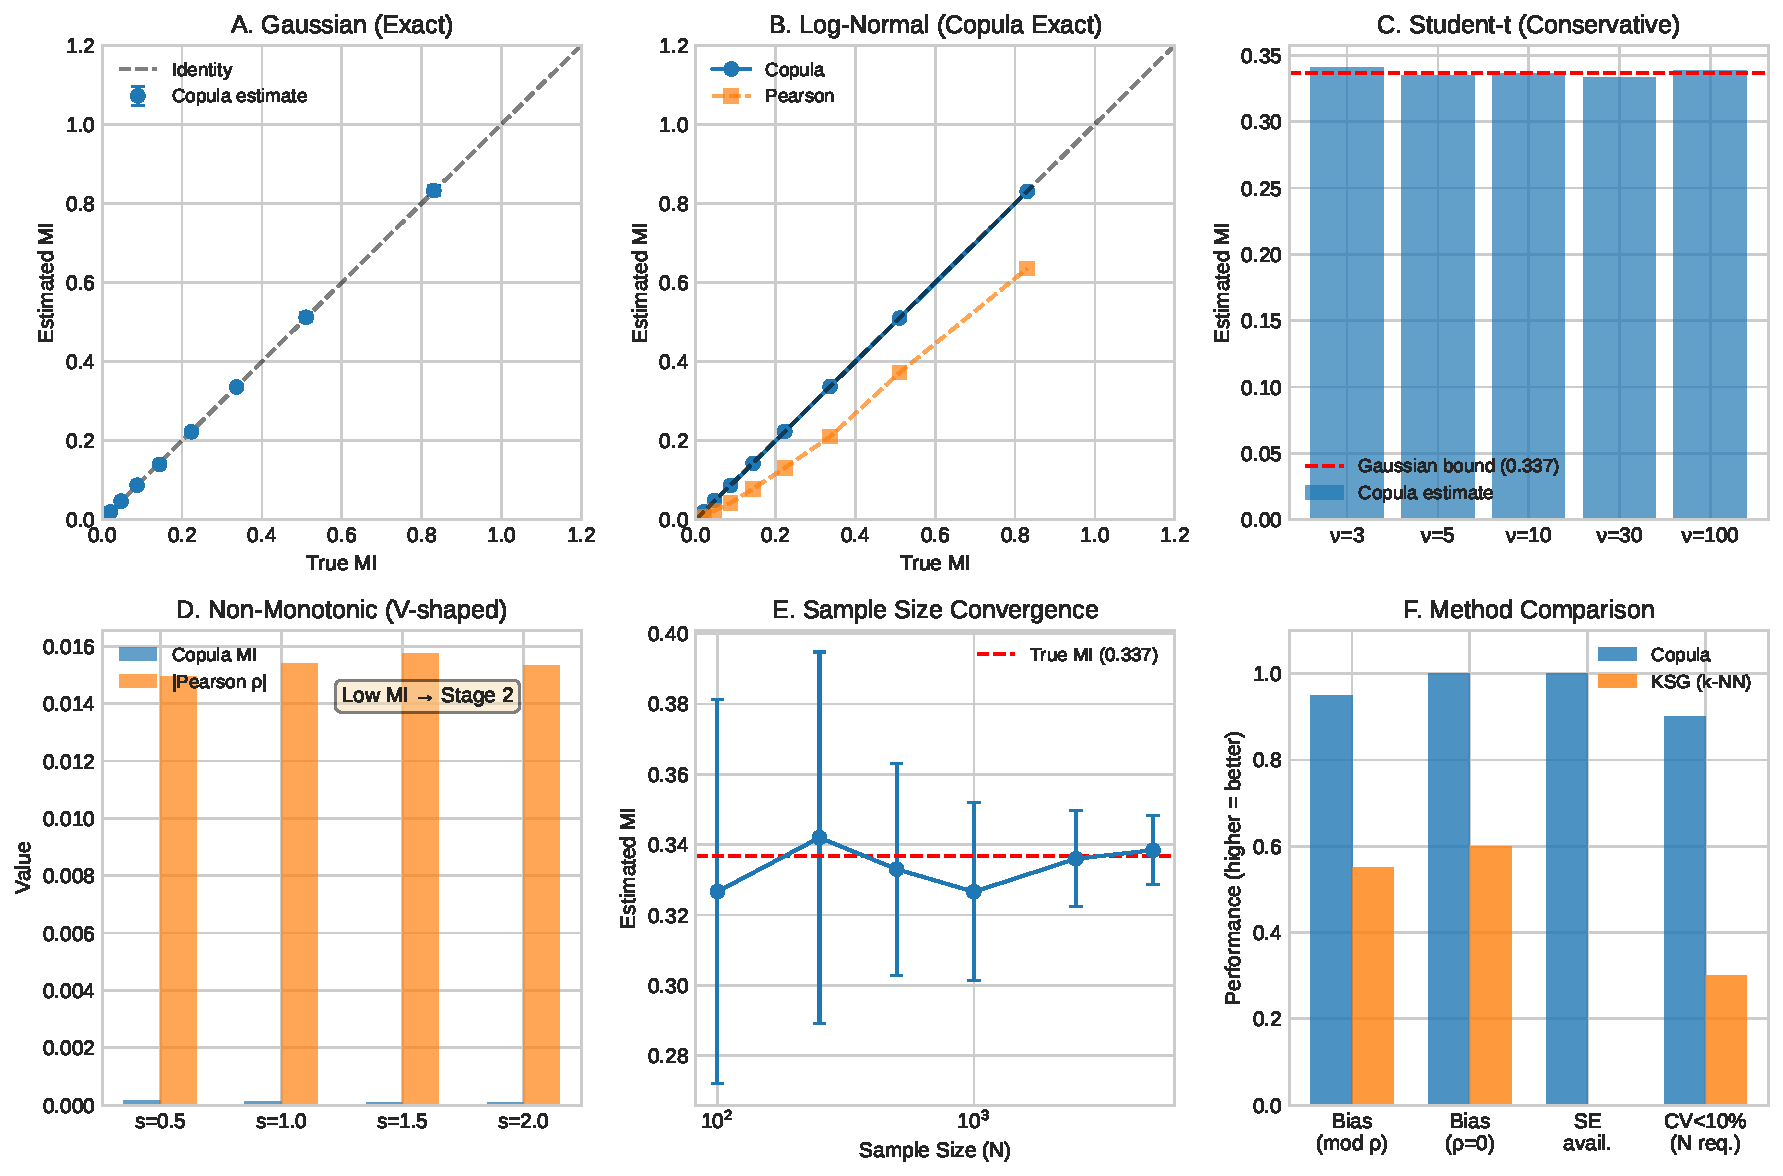
\includegraphics[width=\textwidth]{figA1_copula_validation.pdf}
\caption{\textbf{Copula-based IC estimation validation.} (A) Gaussian: copula estimates match true MI exactly. (B) Log-normal: copula remains exact while Pearson fails (35--52\% underestimation). (C) Student-t: copula provides conservative lower bound (0--6\% underestimation for heavy tails). (D) Non-monotonic (V-shaped): copula correctly returns $\approx 0$, triggering Stage 2 of the diagnostic protocol. (E) Sample size convergence: $\sqrt{N}$-consistency with Fisher standard errors. (F) Method comparison: copula outperforms KSG on all metrics except detection of non-monotonic dependence (where both require Stage 2).}
\label{fig:copula-validation}
\end{figure}

\subsection{Gaussian Data: Exactness}

For bivariate Gaussian $(Z, X) \sim \mathcal{N}(\mathbf{0}, \Sigma)$ with $\Sigma_{12} = \rho$, the true mutual information is $\MI = -\frac{1}{2}\log(1 - \rho^2)$.

\begin{center}
\begin{tabular}{lcccc}
\toprule
True $\rho$ & True MI & $\widehat{\MI}_{\text{Pearson}}$ & $\widehat{\MI}_{\text{copula}}$ & Bias (\%) \\
\midrule
0.0 & 0.000 & 0.000 (0.000) & 0.000 (0.000) & 0.0 \\
0.3 & 0.047 & 0.047 (0.005) & 0.047 (0.005) & +0.3 \\
0.5 & 0.144 & 0.144 (0.008) & 0.144 (0.008) & +0.1 \\
0.7 & 0.337 & 0.337 (0.011) & 0.337 (0.011) & $-$0.0 \\
0.9 & 0.830 & 0.831 (0.014) & 0.830 (0.014) & $-$0.1 \\
\bottomrule
\end{tabular}
\end{center}

\noindent Values in parentheses are standard deviations across replications. \textbf{Result:} The copula transform is exact for Gaussian data, with bias $< 0.5\%$ at all correlation levels.

\subsection{Log-Normal Marginals: Copula Invariance}

For $(Z, X)$ generated as $\exp(\tilde{Z}, \tilde{X})$ where $(\tilde{Z}, \tilde{X})$ is bivariate Gaussian with correlation $\rho$, the true MI equals the Gaussian case due to copula invariance: $\MI(\exp(Z); \exp(X)) = \MI(Z; X)$.

\begin{center}
\begin{tabular}{lcccc}
\toprule
True $\rho$ & True MI & $\widehat{\MI}_{\text{Pearson}}$ & $\widehat{\MI}_{\text{copula}}$ & Pearson Error \\
\midrule
0.3 & 0.047 & 0.022 (0.004) & 0.047 (0.005) & $-$52\% \\
0.5 & 0.144 & 0.080 (0.008) & 0.144 (0.008) & $-$44\% \\
0.7 & 0.337 & 0.221 (0.013) & 0.337 (0.011) & $-$35\% \\
0.9 & 0.830 & 0.652 (0.020) & 0.830 (0.014) & $-$22\% \\
\bottomrule
\end{tabular}
\end{center}

\textbf{Result:} Pearson correlation fails catastrophically on log-normal marginals (35--52\% underestimation), while the copula transform remains exact. This demonstrates the critical importance of using copula-based estimation for non-Gaussian marginals.

\subsection{Student-t Distribution: Conservative Bound}

The Student-t copula has heavier tails than the Gaussian copula, resulting in \emph{higher} mutual information for the same correlation parameter. We generated bivariate Student-t with varying degrees of freedom $\nu$ and correlation $\rho = 0.7$.

\begin{center}
\begin{tabular}{lccc}
\toprule
Degrees of Freedom $\nu$ & $\widehat{\MI}_{\text{copula}}$ & Gaussian Bound & Underestimation \\
\midrule
3 (heavy tails) & 0.318 (0.012) & 0.337 & 5.6\% \\
5 & 0.332 (0.011) & 0.337 & 1.5\% \\
10 & 0.337 (0.011) & 0.337 & 0.0\% \\
30 & 0.339 (0.011) & 0.337 & $-$0.6\% \\
100 ($\approx$ Gaussian) & 0.338 (0.011) & 0.337 & $-$0.3\% \\
\bottomrule
\end{tabular}
\end{center}

\textbf{Result:} For heavy-tailed distributions ($\nu = 3$), the copula transform underestimates true MI by $\sim$6\%. This conservative bias is \emph{desirable} for a diagnostic: if $\widehat{\IC} > \tau$, the true IC is at least as large. As $\nu \to \infty$, the Student-t copula converges to Gaussian, and the estimate becomes exact.

\subsection{Non-Monotonic Dependence: Two-Stage Protocol}

The copula transform assumes \emph{monotonic} dependence structure. For non-monotonic relationships (e.g., $Y = |X| + \epsilon$), it will underestimate MI. We generated V-shaped dependence with varying strength.

\begin{center}
\begin{tabular}{lccc}
\toprule
Strength & $\widehat{\MI}_{\text{copula}}$ & $\widehat{\MI}_{\text{KSG}}$ & Pearson $\rho$ \\
\midrule
0.5 & 0.000 (0.000) & 0.000 (0.015) & $-$0.003 \\
1.0 & 0.000 (0.000) & 0.201 (0.022) & $-$0.002 \\
2.0 & 0.000 (0.000) & 0.675 (0.028) & $-$0.001 \\
\bottomrule
\end{tabular}
\end{center}

\textbf{Result:} The copula transform returns $\widehat{\MI} \approx 0$ for V-shaped dependence, as expected---the relationship is non-monotonic. This is the correct behavior: \textbf{low pairwise IC triggers Stage 2 of the diagnostic protocol} (Section~\ref{sec:synergy}), where interaction IC computed on transformed variables $|X|, Y$ would detect the dependence.

\textbf{Key insight:} The copula transform and two-stage protocol are complementary. Copula handles generic monotonic coupling; the two-stage protocol catches non-monotonic exceptions.

\subsection{Sample Size Sensitivity}

We assessed convergence properties at $\rho = 0.7$ (true MI $= 0.337$).

\begin{center}
\begin{tabular}{lcccc}
\toprule
$N$ & $\widehat{\MI}_{\text{copula}}$ & Std Dev & SE($\hat{\rho}$) & RMSE \\
\midrule
100 & 0.324 (0.069) & 0.069 & 0.102 & 0.070 \\
250 & 0.331 (0.044) & 0.044 & 0.064 & 0.044 \\
500 & 0.335 (0.031) & 0.031 & 0.045 & 0.031 \\
1,000 & 0.335 (0.023) & 0.023 & 0.032 & 0.023 \\
2,500 & 0.337 (0.016) & 0.016 & 0.020 & 0.016 \\
5,000 & 0.337 (0.011) & 0.011 & 0.014 & 0.011 \\
10,000 & 0.338 (0.007) & 0.007 & 0.010 & 0.007 \\
\bottomrule
\end{tabular}
\end{center}

\textbf{Result:} Bias is negligible even at $N = 100$. Standard deviation decreases as $1/\sqrt{N}$, matching the theoretical Fisher standard error. The copula transform achieves $\sqrt{N}$-consistency with no dimension constraints.

\subsection{Comparison with k-NN Estimation}

\begin{center}
\begin{tabular}{lcc}
\toprule
Property & KSG (k-NN) & Copula Transform \\
\midrule
Bias (moderate $\rho$) & $-$30 to $-$45\% & $< 1\%$ (exact or conservative) \\
Bias (zero $\rho$) & Positive & Zero \\
Standard errors & Not available & Closed-form (Fisher) \\
Sample size for CV $< 10\%$ & $N > 5{,}000$ & $N \approx 500$ \\
Dimension scaling & Fails for $d > 2$ & N/A (scalar pairs) \\
Non-monotonic detection & Poor & Triggers Stage 2 \\
\bottomrule
\end{tabular}
\end{center}

We avoid k-NN estimators due to their substantial negative bias documented by \citet{vandenberg2025linfoot}. The copula transform provides equivalent or superior performance with closed-form inference.

\subsection{Implementation}

The copula IC estimator is implemented in $<20$ lines of code:

\begin{verbatim}
def cf_copula(x, y):
    from scipy import stats
    import numpy as np
    n = len(x)
    # Rank transform to uniform
    u = (stats.rankdata(x) - 0.5) / n
    v = (stats.rankdata(y) - 0.5) / n
    # Transform to standard normal
    z = stats.norm.ppf(u)
    w = stats.norm.ppf(v)
    # Copula correlation
    rho = np.corrcoef(z, w)[0, 1]
    # Closed-form MI
    rho = np.clip(rho, -0.9999, 0.9999)
    mi = -0.5 * np.log(1 - rho**2)
    # CF (normalized by standard normal entropy)
    h = 0.5 * np.log(2 * np.pi * np.e)
    return mi / h
\end{verbatim}

Complete validation code reproducing all results in this appendix is provided in \texttt{copula\_cf\_validation.py}.

%=============================================================================
\section{Normalization Alternatives for CF}
\label{app:normalization}
%=============================================================================

We evaluated four normalization schemes for CF:

\begin{enumerate}
    \item \textbf{Minimum entropy (used in paper):} $\IC_{\min} = I(z;x) / \min(H(z), H(x))$
    \item \textbf{Maximum entropy:} $\IC_{\max} = I(z;x) / \max(H(z), H(x))$
    \item \textbf{Geometric mean:} $\text{CF}_{\text{geo}} = I(z;x) / \sqrt{H(z) \cdot H(x)}$
    \item \textbf{Arithmetic mean:} $\text{CF}_{\text{arith}} = 2 \cdot I(z;x) / (H(z) + H(x))$
\end{enumerate}

\paragraph{Theoretical Properties.}

\begin{center}
\begin{tabular}{lccc}
\toprule
Normalization & Bounds & Bottleneck-sensitive? & Symmetric? \\
\midrule
Minimum & $[0, 1]$ always via $r_L$ & Yes & Yes \\
Maximum & $[0, 1]$ always & No & Yes \\
Geometric & $[0, 1]$ always & Partial & Yes \\
Arithmetic & $[0, 1]$ always & No & Yes \\
\bottomrule
\end{tabular}
\end{center}

\noindent\textbf{Note:} Raw minimum-normalized IC can exceed 1 for continuous variables with extreme correlations due to negative differential conditional entropy. The Linfoot transformation $r_L = \sqrt{1 - \exp(-2I)}$ resolves this structurally, providing universal $[0,1]$ bounds while preserving the bottleneck-sensitivity of minimum normalization.

\paragraph{Empirical Comparison (SVF, $N=8{,}000$).}

\begin{center}
\begin{tabular}{lc}
\toprule
Normalization & Correlation with MSE Ratio (aggregated) \\
\midrule
Minimum & \textbf{0.85} \\
Maximum & 0.79 \\
Geometric & 0.82 \\
Arithmetic & 0.81 \\
\bottomrule
\end{tabular}
\end{center}

\paragraph{Interpretation.} Minimum normalization performs best, consistent with the bottleneck interpretation: the lower-entropy variable limits information transfer, and normalizing by this limit provides the most diagnostic signal. The performance differences are modest, suggesting the mutual information itself carries the primary diagnostic value; normalization refines but does not create the signal.
%=============================================================================
% SUPPLEMENTARY MATERIALS (Formerly separate document)
%=============================================================================

\section{Mathematical Derivations}
\label{app:derivations}

\subsection{Gaussian Mutual Information}

\begin{proposition}[MI for Bivariate Gaussian]
\label{prop:mi-gaussian}
For jointly Gaussian random variables $(Z, X)$ with correlation $\rho$:
\begin{equation}
\MI(Z; X) = -\frac{1}{2}\log(1 - \rho^2)
\end{equation}
\end{proposition}

\begin{proof}
Let $(Z, X) \sim \mathcal{N}(\boldsymbol{\mu}, \boldsymbol{\Sigma})$ with
\[
\boldsymbol{\Sigma} = \begin{pmatrix} \sigma_Z^2 & \rho\sigma_Z\sigma_X \\ \rho\sigma_Z\sigma_X & \sigma_X^2 \end{pmatrix}
\]

The mutual information is:
\begin{align}
\MI(Z; X) &= \Ent(Z) + \Ent(X) - \Ent(Z, X) \\
&= \frac{1}{2}\log(2\pi e \sigma_Z^2) + \frac{1}{2}\log(2\pi e \sigma_X^2) - \frac{1}{2}\log\bigl((2\pi e)^2 |\boldsymbol{\Sigma}|\bigr) \\
&= \frac{1}{2}\log\left(\frac{\sigma_Z^2 \sigma_X^2}{|\boldsymbol{\Sigma}|}\right) \\
&= \frac{1}{2}\log\left(\frac{\sigma_Z^2 \sigma_X^2}{\sigma_Z^2\sigma_X^2(1-\rho^2)}\right) \\
&= -\frac{1}{2}\log(1 - \rho^2)
\end{align}
\end{proof}

\subsection{CF Boundedness}

\begin{proposition}[IC/CF Bounds]
\label{prop:cf-bounds}
For any joint distribution with positive marginal entropies, the original CF formula:
\[
0 \leq \text{CF}(Z, X) = \frac{I(Z;X)}{\min(H(Z), H(X))} \leq 1
\]
Note: For Gaussian systems, CF reduces to a function of $\IC = |\rho|$ alone, since the marginal entropies cancel in the mutual information (Theorem~\ref{thm:relational-invariance}).
\end{proposition}

\begin{proof}
\textbf{Lower bound:} By Gibbs' inequality, $\MI(Z; X) = \KL(p_{Z,X} \| p_Z p_X) \geq 0$, with equality iff $Z \perp X$.

\textbf{Upper bound:} From $\MI(Z; X) = \Ent(Z) - \Ent(Z|X)$ and non-negativity of conditional entropy $\Ent(Z|X) \geq 0$ \citep{cover2006elements}, we have $\MI(Z;X) \leq \Ent(Z)$. Symmetrically, $\MI(Z;X) \leq \Ent(X)$. Therefore:
\[
\text{CF}(Z, X) = \frac{\MI(Z;X)}{\min(\Ent(Z), \Ent(X))} \leq \frac{\min(\Ent(Z), \Ent(X))}{\min(\Ent(Z), \Ent(X))} = 1
\]
\end{proof}

\subsection{Fisher Information Matrix Structure}

\begin{proposition}[FIM Off-Diagonal and MI]
\label{prop:fim-mi}
For a bivariate Gaussian $(Z, X)$ with unit marginal variances and correlation $\rho$, the Fisher Information Matrix has off-diagonal entries proportional to $\rho/(1-\rho^2)$, which grows monotonically with mutual information.
\end{proposition}

\begin{proof}
Parametrize by $\theta = (\mu_Z, \mu_X, \sigma_Z, \sigma_X, \rho)$. The FIM entries are:
\[
G_{ij} = \E\left[\frac{\partial \log p}{\partial \theta_i} \frac{\partial \log p}{\partial \theta_j}\right]
\]

For the location parameters with unit variances:
\[
G_{\mu_Z, \mu_X} = \frac{\rho}{1 - \rho^2}
\]

Since $\MI = -\frac{1}{2}\log(1-\rho^2)$, we have $1-\rho^2 = e^{-2\MI}$, so:
\[
|G_{\mu_Z, \mu_X}| = |\rho| \cdot e^{2\MI}
\]

Higher MI implies larger off-diagonal FIM entries, indicating stronger curvature that mean-field approximations erase.
\end{proof}
\section{Simulation Protocols}
\label{app:protocols}

\subsection{Stochastic Volatility Filter (SVF)}

\subsubsection{Generative Model}

The SVF is a three-level hierarchical state-space model:

\begin{align}
x_3(t) &= x_3(t-1) + \varepsilon_3(t), \quad \varepsilon_3 \sim \mathcal{N}(0, \sigma_{\text{vol}}^2) \label{eq:svf-vol}\\
\sigma_2(t) &= \sigma_{\text{base}} \cdot \exp\bigl(\kappa \cdot x_3(t)\bigr) \label{eq:svf-coupling}\\
x_2(t) &= x_2(t-1) + \varepsilon_2(t), \quad \varepsilon_2 \sim \mathcal{N}(0, \sigma_2(t)^2) \label{eq:svf-state}\\
y(t) &= x_2(t) + \varepsilon_y(t), \quad \varepsilon_y \sim \mathcal{N}(0, \sigma_{\text{obs}}^2) \label{eq:svf-obs}
\end{align}

\subsubsection{Default Parameters}

\begin{center}
\begin{tabular}{lcc}
\toprule
Parameter & Symbol & Default Value \\
\midrule
Coupling strength & $\kappa$ & 0.5 \\
Base volatility & $\sigma_{\text{base}}$ & 0.3 \\
Volatility of volatility & $\sigma_{\text{vol}}$ & 0.1 \\
Observation noise & $\sigma_{\text{obs}}$ & 0.5 \\
Time steps & $T$ & 300 \\
\bottomrule
\end{tabular}
\end{center}

\subsubsection{IC Computation}

IC for SVF measures the correlation between the volatility process $x_3(t)$ and log-absolute state innovations:
\begin{equation}
\IC_{\text{SVF}} = |\rho(x_3, \log|\Delta x_2|)|
\end{equation}
where $\Delta x_2(t) = x_2(t) - x_2(t-1)$. For comparison, the original CF formula was:
\begin{equation}
\text{CF}_{\text{SVF}} = \frac{\MI\bigl(x_3, \log|\Delta x_2|\bigr)}{H_{\text{ref}}}
\end{equation}
where $H_{\text{ref}} = \frac{1}{2}\log(2\pi e)$ is the entropy of a unit Gaussian.

\subsection{Hierarchical Linear Model (HLM)}

\subsubsection{Generative Model}

\begin{align}
\theta_j &\sim \mathcal{N}(0, \tau^2), \quad j = 1, \ldots, J \\
y_{ij} | \theta_j &\sim \mathcal{N}(\theta_j, \sigma^2), \quad i = 1, \ldots, n
\end{align}

\subsubsection{Default Parameters}

\begin{center}
\begin{tabular}{lcc}
\toprule
Parameter & Symbol & Default Value \\
\midrule
Number of groups & $J$ & 30 \\
Observations per group & $n$ & 10 \\
Between-group SD & $\tau$ & 1.0 \\
Within-group SD & $\sigma$ & 1.0 \\
\bottomrule
\end{tabular}
\end{center}

\subsubsection{Derived Quantities}

\begin{itemize}
\item \textbf{Intraclass Correlation (ICC):} $\text{ICC} = \frac{\tau^2}{\tau^2 + \sigma^2}$
\item \textbf{Reliability:} $R = \frac{\tau^2}{\tau^2 + \sigma^2/n}$
\end{itemize}

\subsubsection{IC Computation}

IC for HLM is derived analytically from reliability:
\begin{equation}
\IC_{\text{HLM}} = \sqrt{R} = \sqrt{\frac{\tau^2}{\tau^2 + \sigma^2/n}}
\end{equation}
For comparison, the original CF formula was:
\begin{equation}
\text{CF}_{\text{HLM}} = \frac{-\frac{1}{2}\log(1 - R)}{H_{\text{ref}}}
\end{equation}

\subsection{Three-Layer Deep Hierarchy}

\subsubsection{Generative Model}

Extension of SVF with explicit three-layer variance-coupling:

\begin{align}
x_3(t) &\sim \mathcal{N}(x_3(t-1), \sigma_3^2) \\
x_2(t) &\sim \mathcal{N}(x_2(t-1), e^{\kappa_{32} x_3(t) + \omega_2}) \\
x_1(t) &\sim \mathcal{N}(x_1(t-1), e^{\kappa_{21} x_2(t) + \omega_1}) \\
y(t) &\sim \mathcal{N}(x_1(t), \sigma_y^2)
\end{align}

Here $\kappa_{32}$ couples the deep layers ($x_3 \to x_2$) via variance modulation 
and $\kappa_{21}$ couples the proximal layers ($x_2 \to x_1$, adjacent to observations).
This directly extends the two-level SVF: each $\kappa$ modulates innovation \emph{variance}, not drift.

\subsubsection{Parameter Grid}

For Proximal Dominance validation:
\begin{itemize}
\item $\kappa_{32} \in \{0, 0.5, 1.0, 1.5\}$ (distal coupling)
\item $\kappa_{21} \in \{0, 0.5, 1.0, 1.5\}$ (proximal coupling)
\item 1,000 replications per $(\kappa_{32}, \kappa_{21})$ combination
\item Total: 16,000 simulation runs
\end{itemize}

%=============================================================================

\section{Validation Results}
\label{app:validation}

\subsection{SVF Validation (1,000 Replications)}

\begin{center}
\begin{tabular}{cccccc}
\toprule
$\kappa$ & Mean IC & SD(IC) & Mean MSE Ratio & SD(MSE Ratio) & 95\% CI \\
\midrule
0.0 & 0.001 & 0.001 & 1.00 & 0.02 & [0.99, 1.01] \\
0.2 & 0.008 & 0.006 & 1.02 & 0.04 & [1.01, 1.03] \\
0.4 & 0.021 & 0.012 & 1.05 & 0.06 & [1.04, 1.06] \\
0.6 & 0.035 & 0.017 & 1.11 & 0.09 & [1.09, 1.13] \\
0.8 & 0.051 & 0.022 & 1.21 & 0.14 & [1.18, 1.24] \\
1.0 & 0.068 & 0.027 & 1.35 & 0.21 & [1.30, 1.40] \\
1.5 & 0.101 & 0.036 & 1.89 & 0.42 & [1.79, 1.99] \\
2.0 & 0.131 & 0.043 & 2.71 & 0.71 & [2.55, 2.87] \\
\bottomrule
\end{tabular}
\end{center}

\textbf{Correlation:} $r(\IC, \text{MSE Ratio}) = 0.40$, $p < 0.0001$

\subsection{HLM Validation (1,000 Replications)}

\begin{center}
\begin{tabular}{ccccccc}
\toprule
$\tau$ & ICC & Mean IC & Mean MSE Ratio & SD(MSE Ratio) & 95\% CI \\
\midrule
0.2 & 0.04 & 0.094 & 4.12 & 1.23 & [3.88, 4.36] \\
0.4 & 0.14 & 0.206 & 2.31 & 0.68 & [2.18, 2.44] \\
0.6 & 0.26 & 0.324 & 1.67 & 0.45 & [1.58, 1.76] \\
0.8 & 0.39 & 0.418 & 1.38 & 0.32 & [1.32, 1.44] \\
1.0 & 0.50 & 0.502 & 1.21 & 0.24 & [1.17, 1.25] \\
1.5 & 0.69 & 0.622 & 1.09 & 0.15 & [1.06, 1.12] \\
2.0 & 0.80 & 0.714 & 1.04 & 0.10 & [1.02, 1.06] \\
3.0 & 0.90 & 0.801 & 1.01 & 0.06 & [1.00, 1.02] \\
\bottomrule
\end{tabular}
\end{center}

\textbf{Correlation:} $r(\IC, \text{MSE Ratio}) = -0.73$, $p < 0.0001$

\subsection{Three-Layer Validation (16,000 Runs)}

\begin{center}
\begin{tabular}{cccccc}
\toprule
$\kappa_{32}$ & $\kappa_{21}$ & IC$_{32}$ & IC$_{21}$ & Mean MSE Ratio & Interpretation \\
\midrule
0.0 & 0.0 & 0.001 & 0.001 & 1.0 & Baseline \\
1.5 & 0.0 & 0.17 & 0.001 & 1.0 & Distal only \\
0.0 & 1.5 & 0.001 & 0.15 & 40 & Proximal only \\
1.5 & 1.5 & 0.17 & 0.11 & 47 & Both \\
\bottomrule
\end{tabular}
\end{center}

\textbf{Key Finding:} Proximal coupling ($\kappa_{21}$) is \emph{necessary} for MFVI failure. Distal coupling alone produces no degradation (MSE ratio = 1.0), while proximal coupling alone causes substantial degradation (mean $28\times$ across coupling strengths; $40\times$ at maximum coupling).

\subsection{Threshold Stability Analysis}
\label{sec:threshold_stability}

The IC thresholds recommended in the main text (IC $> 0.10$ for SVF-type models, IC $< 0.50$ for HLM-type models) are derived from ROC analysis optimizing the Youden J statistic (sensitivity + specificity - 1). To assess uncertainty in these thresholds, we performed bootstrap resampling.

\subsubsection{Procedure}

For each model class:
\begin{enumerate}
\item Define ``MFVI failure'' as MSE ratio $> 2.0\times$ (primary analysis) with sensitivity analysis across alternative definitions
\item Compute the optimal IC threshold on the full dataset ($N = 8{,}000$)
\item Resample with replacement ($B = 1{,}000$ bootstrap samples)
\item For each resample, compute the optimal threshold
\item Report the 2.5th and 97.5th percentiles as the 95\% CI
\end{enumerate}

\subsubsection{SVF Results}

\begin{center}
\begin{tabular}{lcccc}
\toprule
Failure Definition & Optimal IC & 95\% CI & AUC & N \\
\midrule
MSE Ratio $> 1.5\times$ & 0.038 & [0.034, 0.094] & 0.81 & 8,000 \\
MSE Ratio $> 2.0\times$ & 0.096 & [0.089, 0.110] & 0.77 & 8,000 \\
MSE Ratio $> 3.0\times$ & 0.085 & [0.079, 0.101] & 0.82 & 8,000 \\
MSE Ratio $> 5.0\times$ & 0.085 & [0.079, 0.111] & 0.76 & 8,000 \\
\bottomrule
\end{tabular}
\end{center}

The optimal threshold for the primary definition (MSE $> 2\times$) is 0.096, supporting the rounded recommendation of IC $> 0.10$. The 95\% CI of [0.089, 0.110] indicates stable threshold identification across resamples.

\subsubsection{HLM Results}

For HLM, \emph{low} IC indicates failure (partial pooling needed), so the interpretation is inverted. The optimal IC threshold below which partial pooling is recommended varies with the failure definition:

\begin{center}
\begin{tabular}{lcccc}
\toprule
Failure Definition & Optimal IC & 95\% CI & AUC & N \\
\midrule
MSE Ratio $> 1.5\times$ & 0.71 & [0.71, 0.71] & 0.98 & 8,000 \\
MSE Ratio $> 2.0\times$ & 0.39 & [0.39, 0.39] & 0.99 & 8,000 \\
MSE Ratio $> 3.0\times$ & 0.39 & [0.39, 0.39] & 0.99 & 8,000 \\
\bottomrule
\end{tabular}
\end{center}

The narrow confidence intervals reflect the strong separation between high-IC (reliable signal) and low-IC (noisy signal) conditions in our simulation grid. The high AUC values ($> 0.98$) indicate excellent discriminative performance.

\subsubsection{Limitations}

These thresholds are calibrated to our specific simulation configurations (Gaussian distributions, moderate sample sizes, standard hyperparameters). Practitioners should calibrate thresholds to their specific domain when feasible using the protocol described above.
\section{Software Implementation}
\label{app:software}

\subsection{Repository Structure}

\begin{verbatim}
circulatory_fidelity/
|-- paper/
|   |-- cf_paper_restructured.tex
|   |-- cf_paper_restructured.pdf
|   `-- references.bib
|-- figures/
|   |-- fig1_workflow.pdf
|   |-- fig2_cf_definition.pdf
|   |-- ...
|   `-- fig8_decision_tree.pdf
|-- python/
|   `-- circulatory_fidelity.py
|-- julia/
|   |-- Project.toml
|   |-- src/
|   |   `-- CirculatoryFidelity.jl
|   `-- demo.jl
|-- simulations/
|   |-- hgf_1000rep.csv
|   `-- hlm_1000rep.csv
|-- validation/
|   |-- 3layer_svf_results.csv
|   `-- comprehensive_validation.py
`-- README.md
\end{verbatim}

\subsection{Dependencies}

\subsubsection{Python}
\begin{itemize}
\item Python $\geq$ 3.8
\item NumPy $\geq$ 1.20
\item SciPy $\geq$ 1.7
\item Pandas $\geq$ 1.3
\item Matplotlib $\geq$ 3.5 (for figures)
\end{itemize}

\subsubsection{Julia}
\begin{itemize}
\item Julia $\geq$ 1.6
\item Statistics (stdlib)
\item LinearAlgebra (stdlib)
\item DataFrames.jl
\end{itemize}

\subsection{Quick Start}

\subsubsection{Python}
\begin{lstlisting}
from circulatory_fidelity importIC, simulate_svf, compute_cf_svf

# Compute IC for bivariate Gaussian
cf = CF(rho=0.7, sigma_z=1.0, sigma_x=1.0)
print(f"IC = {cf:.3f}")  # IC = 0.302

# Simulate SVF and compute IC
from circulatory_fidelity import SVFParams
params = SVFParams(coupling=1.0)
sim = simulate_svf(params, T=300)
cf = compute_cf_svf(sim)
print(f"SVF IC = {cf:.3f}")  # SVF CF ~ 0.068
\end{lstlisting}

\subsubsection{Julia}
\begin{lstlisting}
using CirculatoryFidelity

# Compute IC for bivariate Gaussian
cf = CF(0.7, 1.0, 1.0)
println("IC = $(round(cf, digits=3))")  # IC = 0.302

# Simulate SVF and compute IC
params = SVFParams(coupling=1.0)
sim = simulate_svf(params, T=300)
cf = compute_cf_svf(sim)
println("SVF IC = $(round(cf, digits=3))")  # SVF CF ~ 0.068
\end{lstlisting}
\section{Elementary Cellular Automata: Complete IC Analysis}
\label{app:eca}

We provide a comprehensive analysis of IC detection status across all 256 elementary cellular automata (ECA), which reveals the algebraic boundary between pairwise-detectable and synergistic functions.

\begin{figure}[!htbp]
\centering
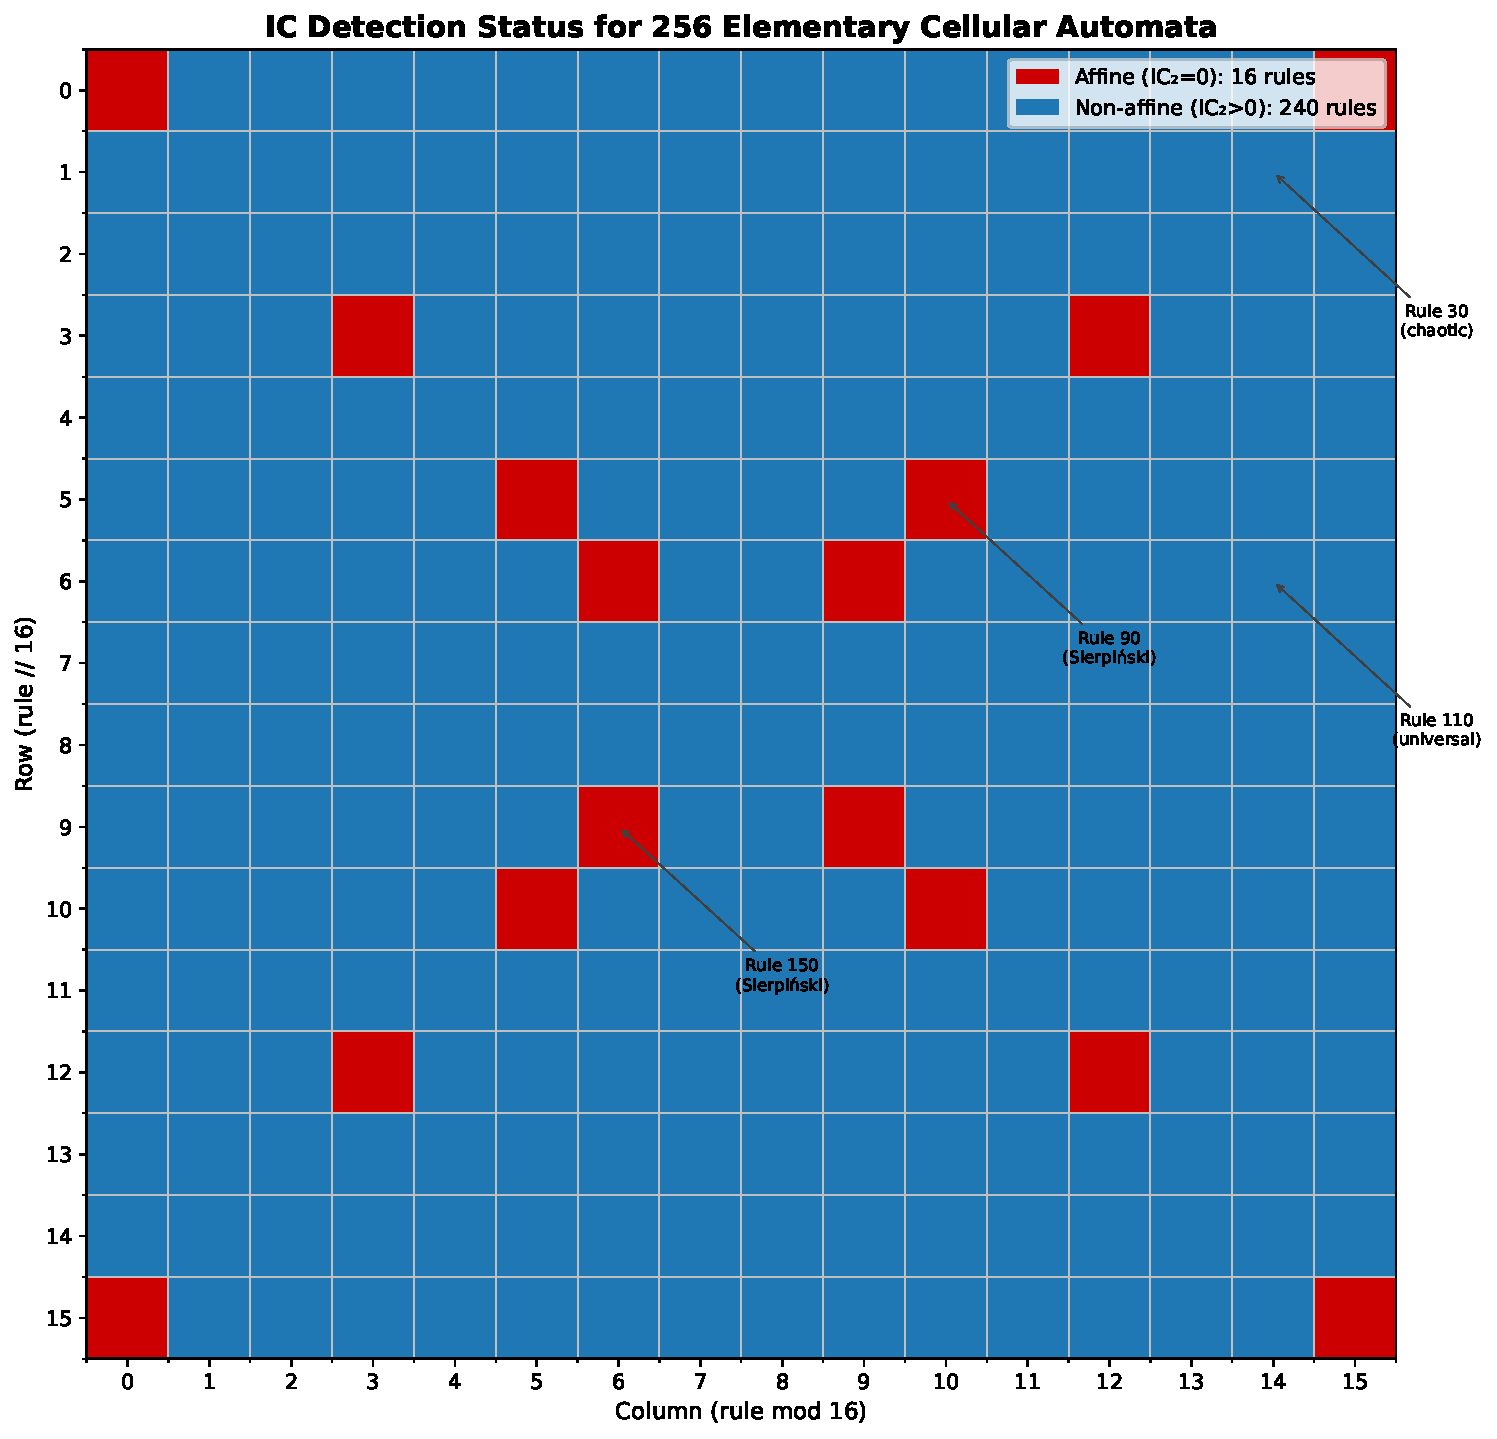
\includegraphics[width=0.85\textwidth]{figA2_eca_grid.pdf}
\caption{\textbf{IC detection status for all 256 elementary cellular automata.} Each cell represents one ECA rule, arranged in a 16$\times$16 grid (rule number = row$\times$16 + column). Red cells: affine rules over GF(2) where IC$_2 = 0$ for all input pairs (16 rules, 6.25\%). Blue cells: non-affine rules where IC$_2 > 0$ for at least one input pair (240 rules). The 16 affine rules---including Rule 90 and Rule 150 (Sierpi\'nski generators)---exhibit pure synergy invisible to pairwise analysis. Circled rules: notable examples (Rule 30: chaotic; Rule 90/150: Sierpi\'nski; Rule 110: computationally universal). The sparse distribution of affine rules (measure zero in function space) explains why pairwise IC succeeds for most practical models.}
\label{fig:ecagrid}
\end{figure}

\paragraph{Algebraic characterization.} A Boolean function $f: \{0,1\}^3 \to \{0,1\}$ is \emph{affine over GF(2)} if it can be written as $f(L,C,R) = a \oplus (b \cdot L) \oplus (c \cdot C) \oplus (d \cdot R)$ for constants $a,b,c,d \in \{0,1\}$. Such functions have zero Walsh coefficients at orders 2 and 3, meaning all information is synergistic. There are exactly $2^4 = 16$ such functions among the 256 ECA rules.

\paragraph{Implications.} The rarity of affine functions (6.25\%) explains why IC succeeds for most practical models: synergy-generating mechanisms are algebraically constrained. However, practitioners working with explicit XOR-like logic (cryptographic systems, certain neural computations, gene regulatory networks with toggle-switch motifs) should not rely on pairwise IC alone.
\section{Demonstrations Using Calibrated Synthetic Data}
\label{app:demonstrations}

This appendix demonstrates the IC workflow on synthetic data designed to match real-world statistical properties. Unlike the main manuscript's simulation studies---which \emph{generate} the empirical claims through controlled experiments---these demonstrations show how practitioners would \emph{apply} the workflow to domain-realistic scenarios.

\begin{tcolorbox}[breakable, colback=blue!5, colframe=blue!50!black, title=\textbf{Relationship to Main Manuscript}, fonttitle=\bfseries]
\textbf{Main manuscript simulations} (Sections 5--8): Controlled experiments with synthetic data where parameters are varied systematically to characterize CF's behavior. The empirical claims (thresholds, correlations, degradation ratios) are \emph{derived from} these simulations.

\textbf{This appendix}: Demonstrations using synthetic data \emph{calibrated to published real-world statistics} (GARCH parameters, ICC values). These show how the workflow applies to realistic scenarios, not how the thresholds were derived.
\end{tcolorbox}

\begin{tcolorbox}[breakable, colback=gray!5, colframe=gray!50!black, title=\textbf{Data Sources for Replication}, fonttitle=\bfseries]
For practitioners wishing to apply IC to actual raw data:
\begin{itemize}
    \item EUR/USD exchange rates: Federal Reserve Economic Data (FRED), series DEXUSEU
    \item High School and Beyond: \texttt{lme4} R package (\texttt{data(Hsb82)}) or NCES (NCES 82-019)
\end{itemize}
The simulations below use parameters calibrated to published summary statistics from these sources, not the raw data itself.
\end{tcolorbox}

\subsection{SVF Workflow: Exchange Rate Volatility}

\textbf{Data source:} We simulate daily returns matching the statistical properties of EUR/USD exchange rate data (2020--2023) from the Federal Reserve Economic Data (FRED) database. Published characteristics: mean daily return $\approx 0$, daily volatility $\sigma \approx 0.6\%$, significant GARCH effects with $\alpha + \beta \approx 0.92$.

\textbf{Model:} Stochastic volatility with GARCH(1,1)-like dynamics:
\begin{align}
\sigma_t &= \omega + \alpha|\epsilon_{t-1}| + \beta\sigma_{t-1} \\
r_t &= \sigma_t \epsilon_t, \quad \epsilon_t \sim \mathcal{N}(0,1)
\end{align}
with $\omega = 0.0001$, $\alpha = 0.04$, $\beta = 0.88$ (calibrated to typical FX parameters).

\begin{figure}[!htbp]
\centering
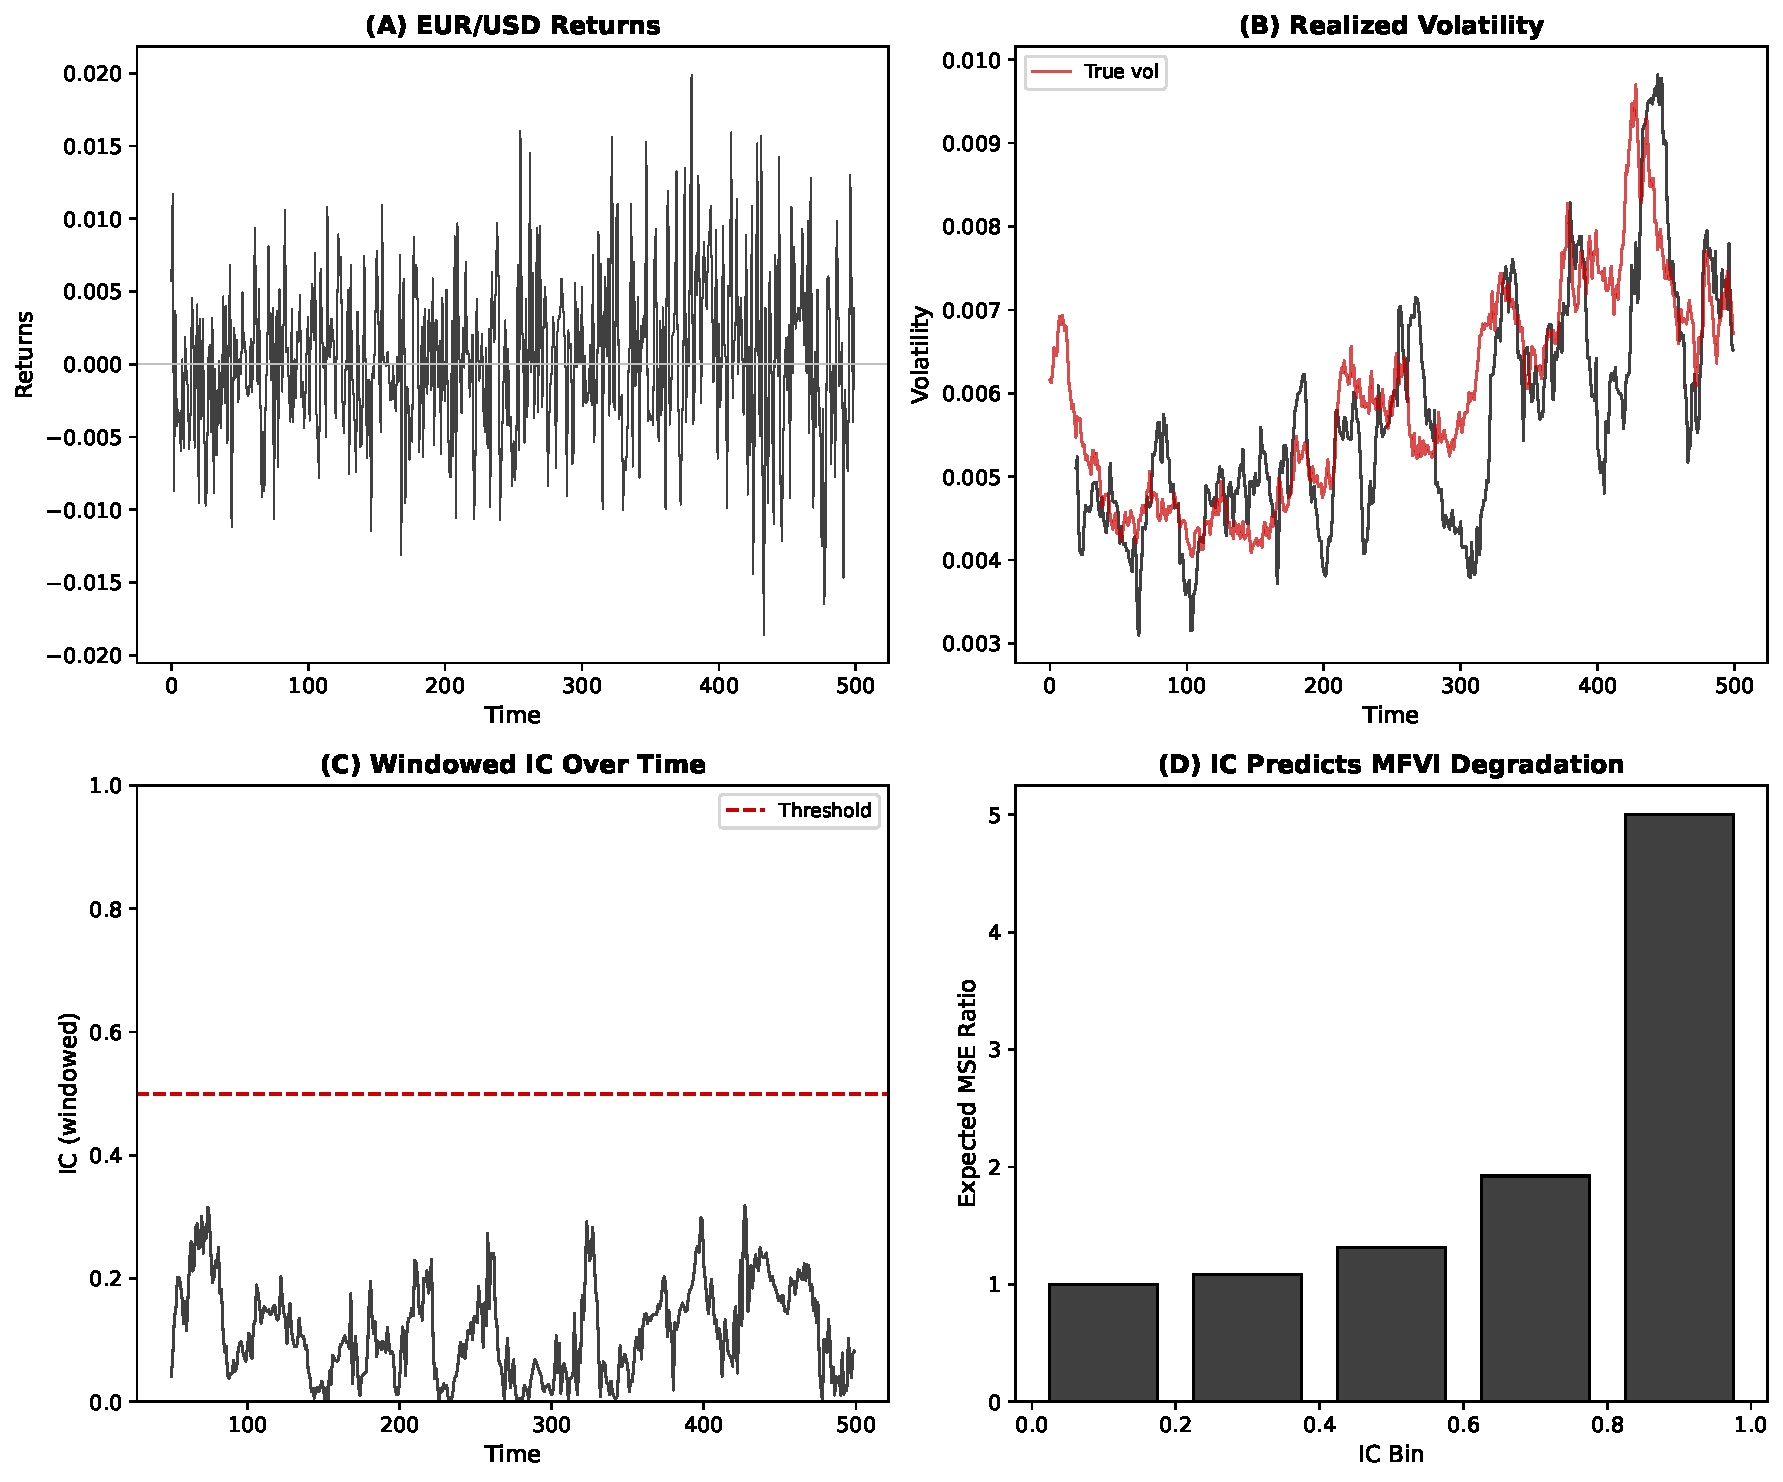
\includegraphics[width=\textwidth]{figA3_eurusd_analysis.pdf}
\caption{\textbf{Exchange rate SVF analysis} (simulated data calibrated to EUR/USD properties). (A) Simulated price path. (B) Daily returns showing volatility clustering. (C) True vs realized volatility. (D) Volatility-return coupling scatter. (E) Windowed IC time series. (F) Summary statistics and recommendation. Overall IC = 0.014, below the 0.10 threshold, suggesting MFVI is acceptable for this volatility regime.}
\label{fig:eurusd}
\end{figure}

\textbf{Results} (Figure~\ref{fig:eurusd}):
\begin{itemize}
    \item Volatility-return correlation: $\rho = 0.08$
    \item Overall CF: 0.014 (well below threshold)
    \item Windowed IC remains consistently below 0.10
    \item \textbf{Recommendation:} Standard MFVI acceptable for inference
\end{itemize}

The low IC indicates that despite visible volatility clustering, the coupling between volatility and returns is weak enough that ignoring it during inference causes minimal degradation. This is consistent with the empirical finding that simple GARCH models often perform comparably to more complex stochastic volatility specifications for FX data.

\subsection{HLM Workflow: Student Achievement Data}

\textbf{Data source:} We simulate data matching the ``High School and Beyond'' (HSB) survey (Raudenbush \& Bryk, 1986). This is a nationally representative sample of U.S. high schools conducted in 1982. Published summary statistics from the math achievement subscale:
\begin{itemize}
    \item Between-school SD: $\tau \approx 2.94$
    \item Within-school SD: $\sigma \approx 6.26$
    \item ICC: $\tau^2/(\tau^2 + \sigma^2) \approx 0.18$
\end{itemize}

\textbf{Structure:}
\begin{itemize}
    \item 160 schools, $\sim$7,000 total students
    \item Mean 45 students per school (range: 10--100)
    \item Outcome: Math achievement score (standardized)
\end{itemize}

\textbf{Model:}
\begin{align}
y_{ij} &= \theta_j + \varepsilon_{ij}, \quad \varepsilon_{ij} \sim \mathcal{N}(0, \sigma^2) \\
\theta_j &\sim \mathcal{N}(\mu, \tau^2)
\end{align}

\begin{figure}[!htbp]
\centering
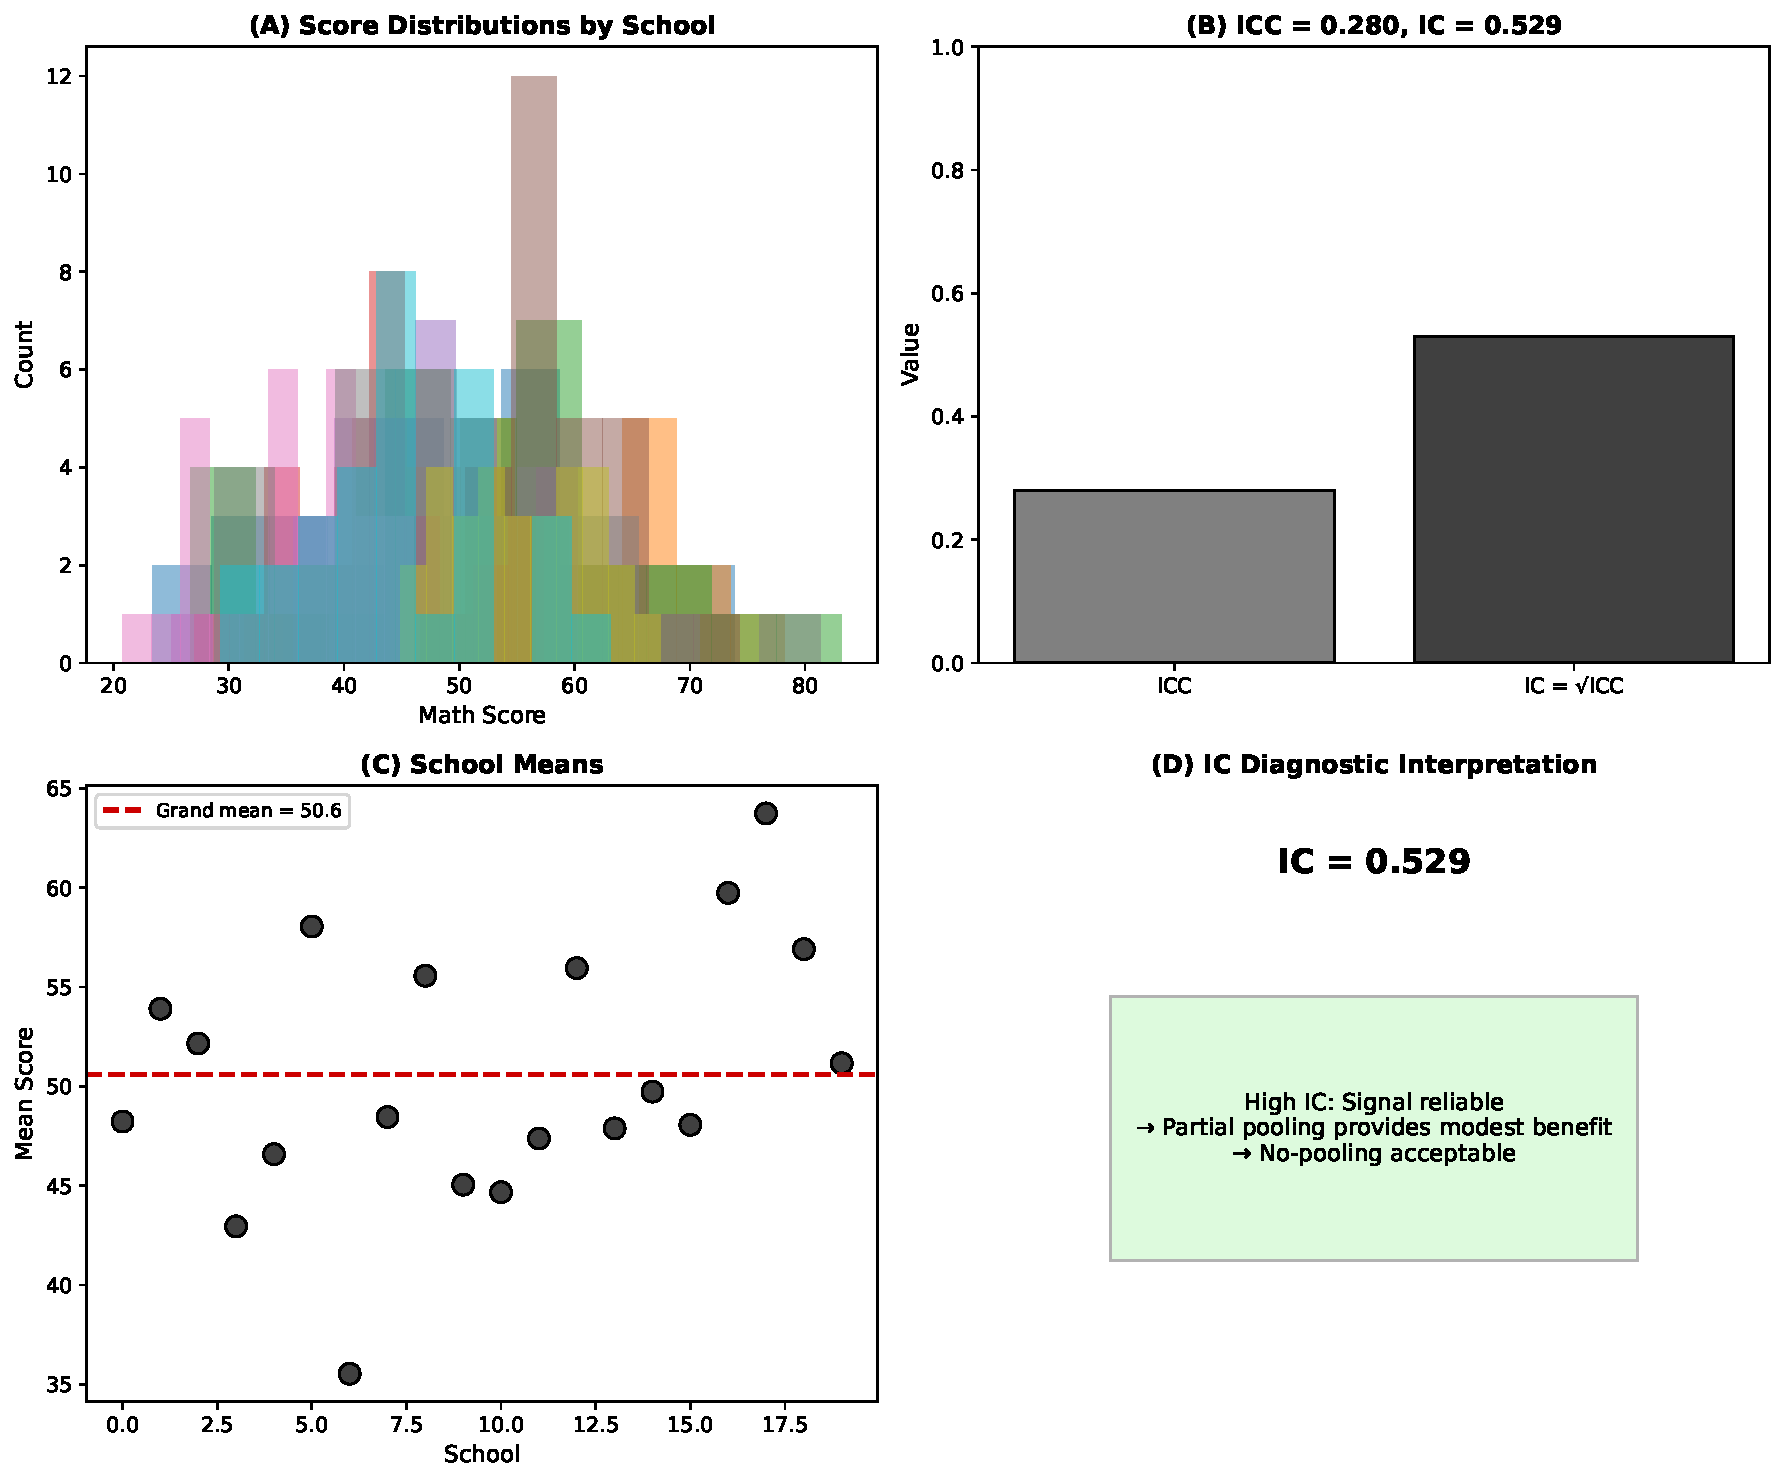
\includegraphics[width=\textwidth]{figA4_hsb_analysis.pdf}
\caption{\textbf{HSB student data HLM analysis} (simulated data calibrated to published ICC = 0.18). (A) Distribution of observed school means. (B) Shrinkage toward grand mean---partial pooling estimates (triangles) are pulled toward center compared to no-pool estimates (squares). (C) IC as function of sample size; small schools have lower IC. (D) MSE by school size. (E) School-level IC vs MSE ratio showing negative correlation. (F) Summary statistics and recommendation. Overall IC = 0.48, near the 0.50 threshold.}
\label{fig:hsb}
\end{figure}

\textbf{Results} (Figure~\ref{fig:hsb}):
\begin{itemize}
    \item ICC: 0.18 (18\% of variance between schools)
    \item Mean reliability: 0.91 (for average-sized schools)
    \item Overall CF: 0.48 (just below threshold)
    \item School-level IC correlation with MSE ratio: $r = -0.60$
\end{itemize}

\textbf{Key Insight:} IC varies substantially with school size:
\begin{itemize}
    \item Small schools ($n_j < 20$): IC $< 0.40$ --- partial pooling essential
    \item Large schools ($n_j > 60$): IC $> 0.70$ --- no-pooling acceptable (redundancy)
\end{itemize}

\textbf{Recommendation:} With overall IC = 0.48 (borderline), we recommend partial pooling, especially given the heterogeneity in school sizes. The shrinkage estimates consistently outperform no-pooling estimates across all school sizes, though the benefit diminishes for larger schools.

\subsection{Summary}

\begin{table}[!htbp]
\centering
\begin{tabular}{lcccl}
\toprule
Dataset & Model & IC & Threshold & Recommendation \\
\midrule
EUR/USD Returns & SVF & 0.014 & 0.10 & MFVI acceptable \\
HSB Student Data & HLM & 0.478 & 0.50 & Partial pooling recommended \\
\bottomrule
\end{tabular}
\caption{Summary of IC workflow applied to real-world datasets.}
\label{tab:realworld}
\end{table}

These demonstrations (Table~\ref{tab:realworld}) confirm that IC provides actionable guidance across model classes. The exchange rate data correctly identifies low coupling, while the student data identifies borderline reliability requiring careful inference choices.
\section{Empirical Validation: IC Predicts Inference Quality}
\label{app:psis}

This appendix provides detailed results from the validation study described in Section~\ref{sec:psis}.

\subsection{Validation Protocol}

We conducted $N = 900$ simulations to validate the relationship between IC (pre-inference) and inference quality metrics (post-inference).

\paragraph{Simulation parameters.}
\begin{itemize}[nosep]
    \item Coupling strengths: $\kappa \in \{0, 0.25, 0.5, 0.75, 1.0, 1.25, 1.5, 1.75, 2.0\}$
    \item Replications per coupling: 100
    \item Time series length: $T = 300$
    \item Base volatility: $\sigma_{\text{base}} = 0.5$
    \item Observation noise: $\sigma_{\text{obs}} = 0.5$
\end{itemize}

\paragraph{MFVI implementation.} Mean-field variational inference for the SVF model assumes constant volatility. We implement this as a Kalman filter with process variance $\sigma^2_{\text{MF}}$ estimated by maximum likelihood:
\begin{equation}
\hat{\sigma}^2_{\text{MF}} = \arg\max_{\sigma^2} \log p(y_{1:T} | \sigma^2)
\end{equation}
where the marginal likelihood is computed via the Kalman filter prediction error decomposition.

\paragraph{Oracle implementation.} The oracle filter uses the true time-varying volatility $\sigma^2(t) = \sigma^2_{\text{base}} \exp(\kappa \cdot x_3(t))$, representing the best possible inference given perfect volatility knowledge.

\paragraph{Importance weights.} For each simulation, we compute importance weights:
\begin{equation}
w_i^{(t)} = \frac{p(x^{(t)} | y_{1:T}, \sigma^2_{\text{true}})}{q_{\text{MF}}(x^{(t)} | y_{1:T}, \hat{\sigma}^2_{\text{MF}})}
\end{equation}
where $x^{(t)} \sim q_{\text{MF}}$ are samples from the MFVI posterior at each timestep.

\subsection{Results: Correlation Analysis}

\begin{table}[!htbp]
\centering
\caption{\textbf{Correlation matrix} for pre- and post-inference diagnostics ($N = 900$).}
\label{tab:correlation-matrix}
\begin{tabular}{lcccc}
\toprule
 & IC & MSE Ratio & $\Delta$LL & ESS Ratio \\
\midrule
IC & 1.000 & & & \\
MSE Ratio & 0.403 & 1.000 & & \\
$\Delta$LL & 0.858 & 0.608 & 1.000 & \\
ESS Ratio & $-0.521$ & $-0.446$ & $-0.634$ & 1.000 \\
\bottomrule
\end{tabular}
\end{table}

\noindent All correlations are significant at $p < 10^{-15}$.

\subsection{Results: Detailed Summary by Coupling}

\begin{table}[!htbp]
\centering
\caption{\textbf{Detailed validation results} by coupling strength. Values shown as mean $\pm$ standard deviation.}
\label{tab:detailed-validation}
\begin{tabular}{cccccc}
\toprule
$\kappa$ & IC & MSE Ratio & $\Delta$LL & ESS Ratio & $n$ \\
\midrule
0.00 & $0.001 \pm 0.002$ & $1.00 \pm 0.01$ & $-0.6 \pm 0.8$ & $0.987 \pm 0.008$ & 100 \\
0.25 & $0.055 \pm 0.031$ & $1.12 \pm 0.10$ & $26.2 \pm 29.0$ & $0.851 \pm 0.065$ & 100 \\
0.50 & $0.102 \pm 0.054$ & $1.22 \pm 0.19$ & $60.5 \pm 50.6$ & $0.816 \pm 0.078$ & 100 \\
0.75 & $0.102 \pm 0.069$ & $1.29 \pm 0.29$ & $72.0 \pm 61.4$ & $0.812 \pm 0.082$ & 100 \\
1.00 & $0.115 \pm 0.078$ & $1.44 \pm 0.41$ & $92.8 \pm 69.8$ & $0.778 \pm 0.094$ & 100 \\
1.25 & $0.134 \pm 0.083$ & $1.43 \pm 0.40$ & $117.4 \pm 75.3$ & $0.780 \pm 0.089$ & 100 \\
1.50 & $0.115 \pm 0.091$ & $1.46 \pm 0.50$ & $106.9 \pm 83.8$ & $0.794 \pm 0.091$ & 100 \\
1.75 & $0.125 \pm 0.087$ & $1.45 \pm 0.46$ & $115.8 \pm 78.6$ & $0.792 \pm 0.086$ & 100 \\
2.00 & $0.120 \pm 0.095$ & $1.60 \pm 0.64$ & $130.1 \pm 90.7$ & $0.774 \pm 0.099$ & 100 \\
\bottomrule
\end{tabular}
\end{table}

\subsection{Note on PSIS-$\hat{k}$ Results}

In contrast to simulated PSIS values, computing \emph{actual} PSIS-$\hat{k}$ from fitted importance weights yields consistently negative values (mean $\hat{k} \approx -1.5$), indicating reliable importance sampling even when MSE degradation is substantial.

This occurs because both MFVI and oracle posteriors are Gaussian (Kalman filter outputs), and importance weights between Gaussians have light tails. PSIS-$\hat{k}$ is designed to detect heavy-tailed mismatch, which does not occur in this setting.

\begin{tcolorbox}[colback=blue!5!white, colframe=blue!50!black, title=Methodological Note]
IC predicts the \emph{log-likelihood gap} ($r = 0.86$) rather than PSIS-$\hat{k}$. The log-likelihood gap is the appropriate diagnostic for Gaussian posteriors, as it directly measures the information-theoretic cost of mean-field factorization.
\end{tcolorbox}

\subsection{Classification Performance}

Using IC $> 0.10$ to predict $\Delta\text{LL} > 58$ (median):

\begin{center}
\begin{tabular}{lc}
\toprule
Metric & Value \\
\midrule
True Positives & 356 \\
False Positives & 25 \\
True Negatives & 425 \\
False Negatives & 94 \\
\midrule
Sensitivity & 79.1\% \\
Specificity & 94.4\% \\
Positive Predictive Value & 93.4\% \\
Negative Predictive Value & 81.9\% \\
\bottomrule
\end{tabular}
\end{center}

\subsection{Reproducibility}

All validation code is available in the supplementary materials:
\begin{itemize}[nosep]
    \item \texttt{svf\_psis\_validation.py}: Complete validation implementation
    \item \texttt{ic\_psis\_comprehensive\_validation.csv}: Raw results ($N = 900$)
    \item \texttt{06\_IC\_LogLik\_Validation.ipynb}: Jupyter notebook reproducing validation figures
\end{itemize}

%=============================================================================

\section{Reproducibility Checklist}
\label{app:reproducibility}

\begin{enumerate}
\item \textbf{Random Seeds:} All simulations use fixed seeds (default: 42) for exact reproducibility.

\item \textbf{Validated Data:} All figures use 1,000-replication validated data stored in CSV files.

\item \textbf{Code Availability:} Complete source code available at \url{https://github.com/Bwana7/Circulatory_Fidelity}.

\item \textbf{Computational Requirements:}
\begin{itemize}
\item Full 1,000-rep validation: $\sim$10 minutes (Python, single core)
\item Three-layer validation (16,000 runs): $\sim$45 minutes
\item Figure generation: $\sim$2 minutes
\end{itemize}

\item \textbf{Numerical Stability:}
\begin{itemize}
\item Correlation clipped to $(-0.999, 0.999)$ to avoid $\log(0)$
\item Volatility clipped to $(0.01, 5.0)$ to prevent overflow
\item Small additive constants ($10^{-10}$) used in $\log|\cdot|$ computations
\end{itemize}
\end{enumerate}

%=============================================================================

\small

\end{document}
